\documentclass[a4paper, openany]{book}
%\documentclass{tuftebook}
\usepackage{amsthm}
\usepackage[many]{tcolorbox}

\makeatletter

\makeatletter

\def\renewtheorem#1{%
	\expandafter\let\csname#1\endcsname\relax
	\expandafter\let\csname c@#1\endcsname\relax
	\gdef\renewtheorem@envname{#1}
	\renewtheorem@secpar
}
\def\renewtheorem@secpar{\@ifnextchar[{\renewtheorem@numberedlike}{\renewtheorem@nonumberedlike}}
\def\renewtheorem@numberedlike[#1]#2{\newtheorem{\renewtheorem@envname}[#1]{#2}}
\def\renewtheorem@nonumberedlike#1{
	\def\renewtheorem@caption{#1}
	\edef\renewtheorem@nowithin{\noexpand\newtheorem{\renewtheorem@envname}{\renewtheorem@caption}}
	\renewtheorem@thirdpar
}
\def\renewtheorem@thirdpar{\@ifnextchar[{\renewtheorem@within}{\renewtheorem@nowithin}}
\def\renewtheorem@within[#1]{\renewtheorem@nowithin[#1]}

\makeatother

%%%%%%%%%%%%%%%%%%%%
% New environments %
%%%%%%%%%%%%%%%%%%%%

\makeatother
%\mdfsetup{skipabove=1em,skipbelow=0em}

\tcbuselibrary{skins}

% Color definitions

\definecolor{proofcolor}{RGB}{0,0,0}

% Dark orange and Dark Red rgb
\definecolor{theorembordercolor}{RGB}{151, 63, 5}
\definecolor{theorembackgroundcolor}{RGB}{248, 241, 234}

\definecolor{examplebordercolor}{RGB}{0, 110, 184}
\definecolor{examplebackgroundcolor}{RGB}{240, 244, 250}

\definecolor{definitionbordercolor}{RGB}{0, 150, 85}
\definecolor{definitionbackgroundcolor}{RGB}{239, 247, 243}

\definecolor{propertybordercolor}{RGB}{128, 0, 128}
\definecolor{propertybackgroundcolor}{RGB}{255, 240, 255}

\definecolor{formulabordercolor}{RGB}{0, 0, 0}
\definecolor{formulabackgroundcolor}{RGB}{230, 229, 245}

\newtheoremstyle{theorem}
{0pt}{0pt}{\normalfont}{0pt}
{}{\;}{0.25em}
{{\sffamily\bfseries\color{theorembordercolor}\thmname{#1}~\thmnumber{\textup{#2}}.}
	\thmnote{\normalfont\color{black}~(#3)}}

\newtheoremstyle{definition}
{0pt}{0pt}{\normalfont}{0pt}
{}{\;}{0.25em}
{{\sffamily\bfseries\color{definitionbordercolor}\thmname{#1}~\thmnumber{\textup{#2}}.}
	\thmnote{\normalfont\color{black}~(#3)}}

\newtheoremstyle{example}
{0pt}{0pt}{\normalfont}{0pt}
{}{\;}{0.25em}
{{\sffamily\bfseries\color{examplebordercolor}\thmname{#1}.}
	\thmnote{\normalfont\color{black}~(#3)}}

\newtheoremstyle{property}
{0pt}{0pt}{\normalfont}{0pt}
{}{\;}{0.25em}
{{\sffamily\bfseries\color{propertybordercolor}\thmname{#1}~\thmnumber{\textup{#2}}.}
	\thmnote{\normalfont\color{black}~(#3)}}

\newtheoremstyle{formula}
{0pt}{0pt}{\normalfont}{0pt}
{}{\;}{0.25em}
{{\sffamily\bfseries\color{formulabordercolor}\thmname{#1}~\thmnumber{\textup{#2}}.}
	\thmnote{\normalfont\color{black}~(#3)}}

%%%%%%%%%%%%%%%%%%%%%%%%
% Theorem Environments %
%%%%%%%%%%%%%%%%%%%%%%%%

\theoremstyle{theorem}

\newtheorem{theorem}{Theorem}
\newtheorem{postulate}{Postulate}
\newtheorem{conjecture}{Conjecture}
\newtheorem{corollary}{Corollary}
\newtheorem{lemma}{Lemma}
\newtheorem{conclusion}{Conclusion}

\tcolorboxenvironment{theorem}{
	enhanced jigsaw, pad at break*=1mm, breakable,
	left=4mm, right=4mm, top=1mm, bottom=1mm,
	colback=theorembackgroundcolor, boxrule=0pt, frame hidden,
	borderline west={0.5mm}{0mm}{theorembordercolor}, arc=.5mm
}
\tcolorboxenvironment{postulate}{
	enhanced jigsaw, pad at break*=1mm, breakable,
	left=4mm, right=4mm, top=1mm, bottom=1mm,
	colback=theorembackgroundcolor, boxrule=0pt, frame hidden,
	borderline west={0.5mm}{0mm}{theorembordercolor}, arc=.5mm
}
\tcolorboxenvironment{conjecture}{
	enhanced jigsaw, pad at break*=1mm, breakable,
	left=4mm, right=4mm, top=1mm, bottom=1mm,
	colback=theorembackgroundcolor, boxrule=0pt, frame hidden,
	borderline west={0.5mm}{0mm}{theorembordercolor}, arc=.5mm
}
\tcolorboxenvironment{corollary}{
	enhanced jigsaw, pad at break*=1mm, breakable,
	left=4mm, right=4mm, top=1mm, bottom=1mm,
	colback=theorembackgroundcolor, boxrule=0pt, frame hidden,
	borderline west={0.5mm}{0mm}{theorembordercolor}, arc=.5mm
}
\tcolorboxenvironment{lemma}{
	enhanced jigsaw, pad at break*=1mm, breakable,
	left=4mm, right=4mm, top=1mm, bottom=1mm,
	colback=theorembackgroundcolor, boxrule=0pt, frame hidden,
	borderline west={0.5mm}{0mm}{theorembordercolor}, arc=.5mm
}
\tcolorboxenvironment{conclusion}{
	enhanced jigsaw, pad at break*=1mm, breakable,
	left=4mm, right=4mm, top=1mm, bottom=1mm,
	colback=theorembackgroundcolor, boxrule=0pt, frame hidden,
	borderline west={0.5mm}{0mm}{theorembordercolor}, arc=.5mm
}

%%%%%%%%%%%%%%%%%%%%%%%%%%%
% Definition Environments %
%%%%%%%%%%%%%%%%%%%%%%%%%%%

\theoremstyle{definition}
\newtheorem{definition}{Definition}
\newtheorem{review}{Review}

\tcolorboxenvironment{definition}{
	enhanced jigsaw, pad at break*=1mm, breakable,
	left=4mm, right=4mm, top=1mm, bottom=1mm,
	colback=definitionbackgroundcolor, boxrule=0pt, frame hidden,
	borderline west={0.5mm}{0mm}{definitionbordercolor}, arc=.5mm
}
\tcolorboxenvironment{review}{
	enhanced jigsaw, pad at break*=1mm, breakable,
	left=4mm, right=4mm, top=1mm, bottom=1mm,
	colback=definitionbackgroundcolor, boxrule=0pt, frame hidden,
	borderline west={0.5mm}{0mm}{definitionbordercolor}, arc=.5mm
}


%%%%%%%%%%%%%%%%%%%%%%%%
% Example Environments %
%%%%%%%%%%%%%%%%%%%%%%%%

\theoremstyle{example}
\newtheorem*{example}{Example}
\newtheorem*{remark}{Remark}
\newtheorem*{note}{Note}

\tcolorboxenvironment{example}{
	enhanced jigsaw, pad at break*=1mm, breakable,
	left=4mm, right=4mm, top=1mm, bottom=1mm,
	colback=examplebackgroundcolor, boxrule=0pt, frame hidden,
	borderline west={0.5mm}{0mm}{examplebordercolor}, arc=.5mm
}
\tcolorboxenvironment{remark}{
	enhanced jigsaw, pad at break*=1mm, breakable,
	left=4mm, right=4mm, top=1mm, bottom=1mm,
	colback=white, boxrule=0pt, frame hidden,
	borderline west={0.5mm}{0mm}{examplebordercolor}, arc=.5mm
}
\tcolorboxenvironment{note}{
	enhanced jigsaw, pad at break*=1mm, breakable,
	left=4mm, right=4mm, top=1mm, bottom=1mm,
	colback=white, boxrule=0pt, frame hidden,
	borderline west={0.5mm}{0mm}{examplebordercolor}, arc=.5mm
}


%%%%%%%%%%%%%%%%%%%%%%%%%
% Property Environments %
%%%%%%%%%%%%%%%%%%%%%%%%%

\theoremstyle{property}
\newtheorem{property}{Property}
\newtheorem{proposition}{Proposition}

\tcolorboxenvironment{property}{
	enhanced jigsaw, pad at break*=1mm, breakable,
	left=4mm, right=4mm, top=1mm, bottom=1mm,
	colback=propertybackgroundcolor, boxrule=0pt, frame hidden,
	borderline west={0.5mm}{0mm}{propertybordercolor}, arc=.5mm
}
\tcolorboxenvironment{proposition}{
	enhanced jigsaw, pad at break*=1mm, breakable,
	left=4mm, right=4mm, top=1mm, bottom=1mm,
	colback=propertybackgroundcolor, boxrule=0pt, frame hidden,
	borderline west={0.5mm}{0mm}{propertybordercolor}, arc=.5mm
}

%%%%%%%%%%%%
% Formula %
%%%%%%%%%%%%

\theoremstyle{formula}
\newtheorem{formula}{Formula}

\tcolorboxenvironment{formula}{
	enhanced jigsaw, pad at break*=1mm, breakable,
	left=4mm, right=4mm, top=1mm, bottom=1mm,
	colback=formulabackgroundcolor, boxrule=0pt, frame hidden,
	borderline west={0.5mm}{0mm}{formulabordercolor}, arc=.5mm
}

%%%%%%%%%
% Proof %
%%%%%%%%%

% These patches must be placed after \tcolorboxenvironment !
\AddToHook{env/theorem/after}{\colorlet{proofcolor}{theorembordercolor}}
\AddToHook{env/postulate/after}{\colorlet{proofcolor}{theorembordercolor}}
\AddToHook{env/conjecture/after}{\colorlet{proofcolor}{theorembordercolor}}
\AddToHook{env/corollary/after}{\colorlet{proofcolor}{theorembordercolor}}
\AddToHook{env/lemma/after}{\colorlet{proofcolor}{theorembordercolor}}
\AddToHook{env/conclusion/after}{\colorlet{proofcolor}{theorembordercolor}}

\AddToHook{env/definition/after}{\colorlet{proofcolor}{definitionbordercolor}}
\AddToHook{env/review/after}{\colorlet{proofcolor}{definitionbordercolor}}

\AddToHook{env/example/after}{\colorlet{proofcolor}{examplebordercolor}}
\AddToHook{env/remark/after}{\colorlet{proofcolor}{examplebordercolor}}
\AddToHook{env/note/after}{\colorlet{proofcolor}{examplebordercolor}}

\AddToHook{env/property/after}{\colorlet{proofcolor}{propertybordercolor}}
\AddToHook{env/proposition/after}{\colorlet{proofcolor}{propertybordercolor}}

\AddToHook{env/formula/after}{\colorlet{proofcolor}{formulabordercolor}}

\renewcommand{\qedsymbol}{Q.E.D.}
\let\qedsymbolMyOriginal\qedsymbol
\renewcommand{\qedsymbol}{
	\color{proofcolor}\qedsymbolMyOriginal
}

\newtheoremstyle{proof}
{0pt}{0pt}{\normalfont}{0pt}
{}{\;}{0.25em}
{{\sffamily\bfseries\color{proofcolor}\thmname{#1}.}
	\thmnote{\normalfont\color{black}~(\textit{#3})}}

\theoremstyle{proof}
\renewtheorem{proof}{Proof}

\tcolorboxenvironment{proof}{
	enhanced jigsaw, pad at break*=1mm, breakable,
	left=4mm, right=4mm, top=1mm, bottom=1mm,
	colback=white, boxrule=0pt, frame hidden,
	borderline west={0.5mm}{0mm}{proofcolor}, arc=.5mm
}

\newenvironment{info}{\begin{tcolorbox}[
		arc=0mm,
		colback=white,
		colframe=gray,
		title=Info,
		fonttitle=\sffamily,
		breakable
		]}{\end{tcolorbox}}
\newenvironment{terminology}{\begin{tcolorbox}[
		arc=0mm,
		colback=white,
		colframe=green!60!black,
		title=Terminology,
		fonttitle=\sffamily,
		breakable
		]}{\end{tcolorbox}}
\newenvironment{warning}{\begin{tcolorbox}[
		arc=0mm,
		colback=white,
		colframe=red,
		title=Warning,
		fonttitle=\sffamily,
		breakable
		]}{\end{tcolorbox}}
\newenvironment{caution}{\begin{tcolorbox}[
		arc=0mm,
		colback=white,
		colframe=yellow,
		title=Caution,
		fonttitle=\sffamily,
		breakable
		]}{\end{tcolorbox}}

\begin{document}
\begin{titlepage}
    \begin{center}
        \line(1,0){300} \\
        [0.25in]
        \huge{\bfseries Math 230A Notes} \\
        [2mm]
        \line(1,0){200} \\
        [1.5cm]
        \textsc{\LARGE Fall, 2024}
    \end{center}
\end{titlepage}

\tableofcontents
\setcounter{section}{0}

\chapter{Defining the Reals}
\section{Defining the Reals}
The main objective of Math 230 is to rigorously explore and generalize many of the concepts learned in calculus such as limits, continuity, sequence convergence, differentiation and integration. 

\begin{remark}
    We aim to uncover the fundamental structures that make calculus possible. For instance, we'll examine what kind of structure is required to discuss the convergence of a sequence within a given set.
    \begin{enumerate}
        \item $\R: ~~~1, \frac{1}{2}, \frac{1}{3}, \frac{1}{4}, ..., \to 0$
        \item $\{\text{blue, dog, pen}\}: ~~~ blue, dog, blue, dog, ... \to ?$
    \end{enumerate}
\end{remark}
\leavevmode \\
In particular, in Math 230A we will be studying:
\begin{enumerate}[1.]
    \item The real numbers
    \item Some aspects of set theory (finite sets, countable sets, ...)
    \item Metric spaces and their topological properties
    \item Sequences and series
    \item Continuous functions between metric spaces
\end{enumerate}
\leavevmode \\
What is a square? There are two ways to answer this question:
\begin{enumerate}[1.]
    \item Show how to construct a square
    \item Identify properties that distinguish a square from any other object in the universe. Defining properties: four sides of equal lengths, rights angles, ...
\end{enumerate}
For this class, we will use 2. to identify the real numbers.

\begin{remark}
    It is possible to 
    \begin{enumerate}
        \item Define the natural numbers $\N$ (equipped with addition and multiplication) using set theory.
        $$1:= \{\emptyset\}, 2:= \{\emptyset, \{\emptyset\}\}, 3:= \{\emptyset, \{\emptyset\}, \{\emptyset, \{\emptyset\}\}\}, ...$$
        \item Then proceed to define the integers $\Z$ as certain equivalence classes with respect to an equivalence relation on $\N \times \N$.
        \item Then define the field of rational numbers $\Q$ as the set of equivalence classes with respect to an equivalence relation on $\Z \times (\Z \backslash \{0\})$.
        \item Then ultimately the field of real numbers.
        \begin{align*}
            &\text{Approach 1: Equivalence classes of Cauchy sequences of rational numbers} \\
            &\text{Approach 2: Dedekind cuts}
        \end{align*}
    \end{enumerate}
\end{remark}

\begin{observation}
    The set $\R$ is not just a boring collection of elements; $\R$ is a set with equipped with extra structures:
    \begin{enumerate}
        \item In $\R$ we have addition and multiplication; addition and multiplication have certain properties.
        $$\text{$\R$ is a field (first defining property)}$$
        \item In $\R$ we have a notion of order.
        $$\text{$\R$ is an ordered field (second defining property)}$$
        \item In fact, $\R$ is the uniqued ordered field that has the least-upper-bound property (third defining property).
        \item In $\R$, there is a notion of length and a corresponding notion of distance.
        \begin{align*}
            &\text{$\R$ is a normed space} \\
            &\text{$\R$ is a metric space}
        \end{align*}
    \end{enumerate}
\end{observation}

\begin{description}
    \item[(I) Elaborating on the first defining property:] 
\end{description}

\begin{definition}[Field] \leavevmode \\
    A field is a set $\mathbb{F}$ with two operations called addition and multiplication, which satisfy the following field-axioms:
    \begin{align*}
        &(A) \text{Addition Axioms} \\
        &(A1) \forall x,y \in \F, ~~x+y \in \F \\
        &(A2) \forall x,y \in \F, ~~x+y = y+x \\
        &(A3) \forall x,y,z \in \F, ~~(x+y)+z = x+(y+z) \\
        &(A4) \F \text{ contains an element $0$ such that $\forall x \in \F, ~0+x = x$} \\
        &(A5) \text{If $x \in \F,$ then there exists an element $-x \in \F \st x + (-x) = 0$}
        \\ \\
        &(M) \text{Multiplication Axioms} \\
        &(M1) \forall x,y \in \F, ~~xy \in \F \\
        &(M2) \forall x,y \in \F, ~~xy = yx \\
        &(M3) \forall x,y,z \in \F ~~(xy)z = x(yz) \\
        &(M4) \F \text{ contains an element $1 \not = 0 \st \forall x \in \F ~x \cdot 1 = x$} \\
        &(M5) \text{If $x \in \F$ and $x \not = 0$, then there exists an element $\frac{1}{x} \in \F \st x \cdot \frac{1}{x} = 1$}
        \\ \\
        &(D) \text{Distributive Law} \\
        &~~~\forall x,y,z \in \F, ~x \cdot (y + z) = x \cdot y + x \cdot z
    \end{align*}
\end{definition}

\begin{description}
    \item[(II) Elaborating on the second defining property:] 
\end{description}
\begin{definition}[Ordered Field] \leavevmode \\
    An ordered field is a field $\F$ equipped with a relation, $<$, with the following properties:
    \begin{enumerate}[$(i)$]
        \item If $x \in \F$ and $y \in \F$, then one and only one of the following statements is true:
        $$x < y, ~y < x, ~x = y$$
        \item If $x,y,z\in \F$ and $x < y$ and $y < z$, then $x < z$.
        \item If $x,y,z \in \F$ and $y < z,$ then $x+y < x+z$.
        \item If $x,y \in \F$, and $0 < x$ and $0 < y$, then $0 < xy$.
    \end{enumerate}
\end{definition}

\begin{remark}
    $\Q$ (the set of rational numbers) is another example of an ordered field (and so, the properties we have discussed is not enough to uniquely identify $\R$).
\end{remark}

\begin{description}
    \item[(III) Elaborating on the third defining property:] 
\end{description}

\begin{definition}[Upper Bounds] \leavevmode \\
    Suppose $\F$ is an ordered field and let $A \subseteq \F.$ If there exists $\beta \in \F \st$
    $$\forall x \in A, ~x \leq \beta$$
    then $\beta$ is called an upper bound of $A$.

    \begin{enumerate}[$*)$]
        \item The collection of all upper bounds of $A$ is denoted by $UP(A)$
        \item If $UP(A) \not = \emptyset$, then we say $A$ is bounded above
    \end{enumerate}
\end{definition}

\begin{definition}[Lower Bounds] \leavevmode \\
    Suppose $\F$ is an ordered field and let $A \subseteq \F.$ If there exists $\alpha \in \F \st$
    $$\forall x \in A, ~\alpha \leq x$$
    then $\alpha$ is called a lower bound of $A$.
    
    \begin{enumerate}[$*)$]
        \item the collection of all the lower bounds of $A$ is denoted by $LO(A)$
        \item If $LO(A) \not = \emptyset,$ then we say $A$ is bounded below
    \end{enumerate}
\end{definition}

\begin{example}
    Let $A = [0,1).$
    $$UP(A) = [1, \infty), ~~LO(A) = (-\infty, 0]$$
\end{example}
\newpage

\section{Supremum and Infimum}
\begin{definition}[Supremum] \leavevmode \\
    Suppose $\F$ is an ordered field and $A\subseteq \F.$ Suppose there exists $\beta \in \F \st$
    \begin{enumerate}[$(i)$]
        \item $\beta \in UP(A)$
        \item If $\gamma \in \F$ and $\gamma < \beta,$ then $\gamma \not \in UP(A)$
    \end{enumerate}
    then we call $\beta$ the least upper bound of $A$, or the supremum of $A$, and we write $\beta = \sup A.$
\end{definition}

\begin{definition}[Infimum] \leavevmode \\
    Suppose $\F$ is an ordered field and $A\subseteq \F.$ Suppose there exists $\alpha \in \F \st$
    \begin{enumerate}[$(i)$]
        \item $\alpha \in LO(A)$
        \item If $\gamma \in \F$ and $\gamma > \alpha,$ then $\gamma \not \in LO(A)$
    \end{enumerate}
    then we call $\alpha$ the greatest lower bound of $A$, or the infimum of $A$, and we write $\alpha = \inf A.$
\end{definition}

\begin{definition}[Least-upper-bound Property] \leavevmode \\
    An ordered field $\F$ is said to have the least-upper-bound property if the following is true:
    $$\text{Every nonempty set $A$ in $\F$ that is bounded above has a least-upper-bound in $\F$}$$
    In other words, if $A \not \emptyset$, then $\sup A$ exists in $\F$.
\end{definition}

\begin{theorem} \leavevmode \\
    There is exactly one ordered field that has the least-upper-bound property. This unique field contains $\Q$ as a subfield.
\end{theorem}

\begin{definition}[The Real Numbers] \leavevmode \\
    The set of real numbers, denoted $\R$, is the unique ordered field that has the least-upper-bound property and contains $\Q$ as a subfield.
\end{definition}

\begin{definition}[Maximum and Minimum] \leavevmode \\
    Let $A \subseteq \R.$

    \begin{enumerate}[$*)$]
        \item If $\sup A\in A$, we call the $\sup A$ the maximum of $A$, denoted $\max A$.
        \item If $\inf A\in A$, we call the $\inf A$ the minimum of $A$, denoted $\min A$.
    \end{enumerate}
    \begin{align*}
        &\sup A = \min UP(A) &&\inf A = \max LO(A)
    \end{align*}
\end{definition}

\begin{fact}[Very Useful Fact] \leavevmode \\
    Let $A \subseteq \R.$
    \begin{enumerate}[1.]
        \item $\beta = \sup A \iff
        \begin{cases*}
            (i) \beta \in UP(A) \\
            (ii) \forall \epsilon > 0, ~\beta - \epsilon \not \in UP(A)
        \end{cases*} \iff
        \begin{cases*}
            (i) \beta \in UP(A) \\
            (ii) \forall \epsilon > 0 ~\exists a \in A \st \beta - \epsilon < a
        \end{cases*}$

        \item $\alpha = \inf A \iff
        \begin{cases*}
            (i) \alpha \in LO(A) \\
            (ii) \forall \epsilon > 0, ~\alpha + \epsilon \not \in LO(A)
        \end{cases*} \iff
        \begin{cases*}
            (i) \alpha \in LO(A) \\
            (ii) \forall \epsilon > 0 ~\exists a \in A \st a < \alpha + \epsilon
        \end{cases*}$
    \end{enumerate}
\end{fact}

\begin{theorem}[Greatest-lower-bound Property of $\R$] \leavevmode \\
    Every nonempty subset $A$ of $\R$ that is bounded below has a greatest upper bound in $\R$.
\end{theorem}

\begin{theorem} [Archimedean Property] \leavevmode \\
    If $x\in \R, ~y\in \R$ and $x > 0$, then there exists a positive integer $n$ such that $nx > y.$
\end{theorem}

\begin{proof}
    Let $A=\{nx : n \in \N\}.$ If the claim were false, then $y$ would be an upper bound for $A$. Then by the least-upper-bound property of $\R$, $A$ has a least upper bound in $\R$. Let $\beta = \sup A$.
    $$\beta = \sup A \implies \forall \epsilon > 0 ~\exists n \in \N ~~\beta - \epsilon < nx.$$
    That is,
    $$\forall \epsilon > 0 ~\exists n \in \N \st \beta < nx + \epsilon.$$
    In particular, if we let $\epsilon = x,$ we can find $m \in \N \st$
    $$\beta < mx + x.$$
    That is $\beta < (m+1)x.$ However, $(m+1)x \in A.$ This contradicts the fact that $\beta$ is an upper bound of $A$.\qed
\end{proof}

\begin{remark} \leavevmode
    (The well-ordering property of the natural numbers) \\
    Every nonempty set of natural numbers has a $\min.$
\end{remark}

\begin{corollary} \leavevmode \\
    Let $A$ be a nonempty subset of $\R$ that consists of only integers.
    \begin{enumerate}[$*)$]
        \item If $A$ is bounded above, then $\sup A \in A.$
        \item If $A$ is bounded below, then $\inf A \in A.$
    \end{enumerate}
\end{corollary}

\begin{theorem}[Density of $\Q$ in $\R$] \leavevmode \\
    For every two real numbers $x$ and $y$ with $x < y$, there exists a rational number $x < p < y$.
\end{theorem}

\begin{proof}
    Recall that $\Q = \{\frac{m}{n} : m \in \Z, ~n \in \N\}.$ Suppose $x \in \R, ~y \in \R$ and $x < y.$ Our goal is to show that there exists an $m \in \Z$ and $n \in \N$ such that $x < \frac{m}{n} < y,$ that is, we want to show that there exists $m \in \Z$ and $n \in \N$ such that $nx < m < ny.$
    \begin{info}
        If we find $n\in \N$ such that it ensures that there is an integer between $nx$ and $ny$, then we are done. To this end, it is enough to find $n \in \N$ such that $ny - nx > 1,$ that is, it is enough to find $n \in \N \st y - x > \frac{1}{n}$.
    \end{info}
    Notice that $y - x > 0.$ Choose $n \in \N \st \frac{1}{n} < y - x$ (by the archimedean property of $\R$, such an $n$ exists). Now, choose $m\in \Z$ to be the smallest integer greater than $nx,$ that is, choose $m\in \Z$ such that 
    $$m-1 \leq nx < m$$
    We have
    \begin{equation*}
        nx < m \implies x < \frac{m}{n} \tag{$I$}
    \end{equation*}
    \begin{equation*}
        m-1 \leq nx \implies m \leq nx + 1 < n(y-\frac{1}{n}) + 1 = ny \implies \frac{m}{n} < y \tag{$II$}
    \end{equation*}
    $(I),(II) \implies x < \frac{m}{n} < y.$ \qed
\end{proof}
\newpage

\chapter{Basic Topology}
\section{Compactness}
\documentclass[a4paper]{article}
%\documentclass{tuftebook}
\usepackage{amsthm}
\usepackage[many]{tcolorbox}

\makeatletter

\makeatletter

\def\renewtheorem#1{%
	\expandafter\let\csname#1\endcsname\relax
	\expandafter\let\csname c@#1\endcsname\relax
	\gdef\renewtheorem@envname{#1}
	\renewtheorem@secpar
}
\def\renewtheorem@secpar{\@ifnextchar[{\renewtheorem@numberedlike}{\renewtheorem@nonumberedlike}}
\def\renewtheorem@numberedlike[#1]#2{\newtheorem{\renewtheorem@envname}[#1]{#2}}
\def\renewtheorem@nonumberedlike#1{
	\def\renewtheorem@caption{#1}
	\edef\renewtheorem@nowithin{\noexpand\newtheorem{\renewtheorem@envname}{\renewtheorem@caption}}
	\renewtheorem@thirdpar
}
\def\renewtheorem@thirdpar{\@ifnextchar[{\renewtheorem@within}{\renewtheorem@nowithin}}
\def\renewtheorem@within[#1]{\renewtheorem@nowithin[#1]}

\makeatother

%%%%%%%%%%%%%%%%%%%%
% New environments %
%%%%%%%%%%%%%%%%%%%%

\makeatother
%\mdfsetup{skipabove=1em,skipbelow=0em}

\tcbuselibrary{skins}

% Color definitions

\definecolor{proofcolor}{RGB}{0,0,0}

% Dark orange and Dark Red rgb
\definecolor{theorembordercolor}{RGB}{151, 63, 5}
\definecolor{theorembackgroundcolor}{RGB}{248, 241, 234}

\definecolor{examplebordercolor}{RGB}{0, 110, 184}
\definecolor{examplebackgroundcolor}{RGB}{240, 244, 250}

\definecolor{definitionbordercolor}{RGB}{0, 150, 85}
\definecolor{definitionbackgroundcolor}{RGB}{239, 247, 243}

\definecolor{propertybordercolor}{RGB}{128, 0, 128}
\definecolor{propertybackgroundcolor}{RGB}{255, 240, 255}

\definecolor{formulabordercolor}{RGB}{0, 0, 0}
\definecolor{formulabackgroundcolor}{RGB}{230, 229, 245}

\newtheoremstyle{theorem}
{0pt}{0pt}{\normalfont}{0pt}
{}{\;}{0.25em}
{{\sffamily\bfseries\color{theorembordercolor}\thmname{#1}~\thmnumber{\textup{#2}}.}
	\thmnote{\normalfont\color{black}~(#3)}}

\newtheoremstyle{definition}
{0pt}{0pt}{\normalfont}{0pt}
{}{\;}{0.25em}
{{\sffamily\bfseries\color{definitionbordercolor}\thmname{#1}~\thmnumber{\textup{#2}}.}
	\thmnote{\normalfont\color{black}~(#3)}}

\newtheoremstyle{example}
{0pt}{0pt}{\normalfont}{0pt}
{}{\;}{0.25em}
{{\sffamily\bfseries\color{examplebordercolor}\thmname{#1}.}
	\thmnote{\normalfont\color{black}~(#3)}}

\newtheoremstyle{property}
{0pt}{0pt}{\normalfont}{0pt}
{}{\;}{0.25em}
{{\sffamily\bfseries\color{propertybordercolor}\thmname{#1}~\thmnumber{\textup{#2}}.}
	\thmnote{\normalfont\color{black}~(#3)}}

\newtheoremstyle{formula}
{0pt}{0pt}{\normalfont}{0pt}
{}{\;}{0.25em}
{{\sffamily\bfseries\color{formulabordercolor}\thmname{#1}~\thmnumber{\textup{#2}}.}
	\thmnote{\normalfont\color{black}~(#3)}}

%%%%%%%%%%%%%%%%%%%%%%%%
% Theorem Environments %
%%%%%%%%%%%%%%%%%%%%%%%%

\theoremstyle{theorem}

\newtheorem{theorem}{Theorem}
\newtheorem{postulate}{Postulate}
\newtheorem{conjecture}{Conjecture}
\newtheorem{corollary}{Corollary}
\newtheorem{lemma}{Lemma}
\newtheorem{conclusion}{Conclusion}

\tcolorboxenvironment{theorem}{
	enhanced jigsaw, pad at break*=1mm, breakable,
	left=4mm, right=4mm, top=1mm, bottom=1mm,
	colback=theorembackgroundcolor, boxrule=0pt, frame hidden,
	borderline west={0.5mm}{0mm}{theorembordercolor}, arc=.5mm
}
\tcolorboxenvironment{postulate}{
	enhanced jigsaw, pad at break*=1mm, breakable,
	left=4mm, right=4mm, top=1mm, bottom=1mm,
	colback=theorembackgroundcolor, boxrule=0pt, frame hidden,
	borderline west={0.5mm}{0mm}{theorembordercolor}, arc=.5mm
}
\tcolorboxenvironment{conjecture}{
	enhanced jigsaw, pad at break*=1mm, breakable,
	left=4mm, right=4mm, top=1mm, bottom=1mm,
	colback=theorembackgroundcolor, boxrule=0pt, frame hidden,
	borderline west={0.5mm}{0mm}{theorembordercolor}, arc=.5mm
}
\tcolorboxenvironment{corollary}{
	enhanced jigsaw, pad at break*=1mm, breakable,
	left=4mm, right=4mm, top=1mm, bottom=1mm,
	colback=theorembackgroundcolor, boxrule=0pt, frame hidden,
	borderline west={0.5mm}{0mm}{theorembordercolor}, arc=.5mm
}
\tcolorboxenvironment{lemma}{
	enhanced jigsaw, pad at break*=1mm, breakable,
	left=4mm, right=4mm, top=1mm, bottom=1mm,
	colback=theorembackgroundcolor, boxrule=0pt, frame hidden,
	borderline west={0.5mm}{0mm}{theorembordercolor}, arc=.5mm
}
\tcolorboxenvironment{conclusion}{
	enhanced jigsaw, pad at break*=1mm, breakable,
	left=4mm, right=4mm, top=1mm, bottom=1mm,
	colback=theorembackgroundcolor, boxrule=0pt, frame hidden,
	borderline west={0.5mm}{0mm}{theorembordercolor}, arc=.5mm
}

%%%%%%%%%%%%%%%%%%%%%%%%%%%
% Definition Environments %
%%%%%%%%%%%%%%%%%%%%%%%%%%%

\theoremstyle{definition}
\newtheorem{definition}{Definition}
\newtheorem{review}{Review}

\tcolorboxenvironment{definition}{
	enhanced jigsaw, pad at break*=1mm, breakable,
	left=4mm, right=4mm, top=1mm, bottom=1mm,
	colback=definitionbackgroundcolor, boxrule=0pt, frame hidden,
	borderline west={0.5mm}{0mm}{definitionbordercolor}, arc=.5mm
}
\tcolorboxenvironment{review}{
	enhanced jigsaw, pad at break*=1mm, breakable,
	left=4mm, right=4mm, top=1mm, bottom=1mm,
	colback=definitionbackgroundcolor, boxrule=0pt, frame hidden,
	borderline west={0.5mm}{0mm}{definitionbordercolor}, arc=.5mm
}


%%%%%%%%%%%%%%%%%%%%%%%%
% Example Environments %
%%%%%%%%%%%%%%%%%%%%%%%%

\theoremstyle{example}
\newtheorem*{example}{Example}
\newtheorem*{remark}{Remark}
\newtheorem*{note}{Note}

\tcolorboxenvironment{example}{
	enhanced jigsaw, pad at break*=1mm, breakable,
	left=4mm, right=4mm, top=1mm, bottom=1mm,
	colback=examplebackgroundcolor, boxrule=0pt, frame hidden,
	borderline west={0.5mm}{0mm}{examplebordercolor}, arc=.5mm
}
\tcolorboxenvironment{remark}{
	enhanced jigsaw, pad at break*=1mm, breakable,
	left=4mm, right=4mm, top=1mm, bottom=1mm,
	colback=white, boxrule=0pt, frame hidden,
	borderline west={0.5mm}{0mm}{examplebordercolor}, arc=.5mm
}
\tcolorboxenvironment{note}{
	enhanced jigsaw, pad at break*=1mm, breakable,
	left=4mm, right=4mm, top=1mm, bottom=1mm,
	colback=white, boxrule=0pt, frame hidden,
	borderline west={0.5mm}{0mm}{examplebordercolor}, arc=.5mm
}


%%%%%%%%%%%%%%%%%%%%%%%%%
% Property Environments %
%%%%%%%%%%%%%%%%%%%%%%%%%

\theoremstyle{property}
\newtheorem{property}{Property}
\newtheorem{proposition}{Proposition}

\tcolorboxenvironment{property}{
	enhanced jigsaw, pad at break*=1mm, breakable,
	left=4mm, right=4mm, top=1mm, bottom=1mm,
	colback=propertybackgroundcolor, boxrule=0pt, frame hidden,
	borderline west={0.5mm}{0mm}{propertybordercolor}, arc=.5mm
}
\tcolorboxenvironment{proposition}{
	enhanced jigsaw, pad at break*=1mm, breakable,
	left=4mm, right=4mm, top=1mm, bottom=1mm,
	colback=propertybackgroundcolor, boxrule=0pt, frame hidden,
	borderline west={0.5mm}{0mm}{propertybordercolor}, arc=.5mm
}

%%%%%%%%%%%%
% Formula %
%%%%%%%%%%%%

\theoremstyle{formula}
\newtheorem{formula}{Formula}

\tcolorboxenvironment{formula}{
	enhanced jigsaw, pad at break*=1mm, breakable,
	left=4mm, right=4mm, top=1mm, bottom=1mm,
	colback=formulabackgroundcolor, boxrule=0pt, frame hidden,
	borderline west={0.5mm}{0mm}{formulabordercolor}, arc=.5mm
}

%%%%%%%%%
% Proof %
%%%%%%%%%

% These patches must be placed after \tcolorboxenvironment !
\AddToHook{env/theorem/after}{\colorlet{proofcolor}{theorembordercolor}}
\AddToHook{env/postulate/after}{\colorlet{proofcolor}{theorembordercolor}}
\AddToHook{env/conjecture/after}{\colorlet{proofcolor}{theorembordercolor}}
\AddToHook{env/corollary/after}{\colorlet{proofcolor}{theorembordercolor}}
\AddToHook{env/lemma/after}{\colorlet{proofcolor}{theorembordercolor}}
\AddToHook{env/conclusion/after}{\colorlet{proofcolor}{theorembordercolor}}

\AddToHook{env/definition/after}{\colorlet{proofcolor}{definitionbordercolor}}
\AddToHook{env/review/after}{\colorlet{proofcolor}{definitionbordercolor}}

\AddToHook{env/example/after}{\colorlet{proofcolor}{examplebordercolor}}
\AddToHook{env/remark/after}{\colorlet{proofcolor}{examplebordercolor}}
\AddToHook{env/note/after}{\colorlet{proofcolor}{examplebordercolor}}

\AddToHook{env/property/after}{\colorlet{proofcolor}{propertybordercolor}}
\AddToHook{env/proposition/after}{\colorlet{proofcolor}{propertybordercolor}}

\AddToHook{env/formula/after}{\colorlet{proofcolor}{formulabordercolor}}

\renewcommand{\qedsymbol}{Q.E.D.}
\let\qedsymbolMyOriginal\qedsymbol
\renewcommand{\qedsymbol}{
	\color{proofcolor}\qedsymbolMyOriginal
}

\newtheoremstyle{proof}
{0pt}{0pt}{\normalfont}{0pt}
{}{\;}{0.25em}
{{\sffamily\bfseries\color{proofcolor}\thmname{#1}.}
	\thmnote{\normalfont\color{black}~(\textit{#3})}}

\theoremstyle{proof}
\renewtheorem{proof}{Proof}

\tcolorboxenvironment{proof}{
	enhanced jigsaw, pad at break*=1mm, breakable,
	left=4mm, right=4mm, top=1mm, bottom=1mm,
	colback=white, boxrule=0pt, frame hidden,
	borderline west={0.5mm}{0mm}{proofcolor}, arc=.5mm
}

\newenvironment{info}{\begin{tcolorbox}[
		arc=0mm,
		colback=white,
		colframe=gray,
		title=Info,
		fonttitle=\sffamily,
		breakable
		]}{\end{tcolorbox}}
\newenvironment{terminology}{\begin{tcolorbox}[
		arc=0mm,
		colback=white,
		colframe=green!60!black,
		title=Terminology,
		fonttitle=\sffamily,
		breakable
		]}{\end{tcolorbox}}
\newenvironment{warning}{\begin{tcolorbox}[
		arc=0mm,
		colback=white,
		colframe=red,
		title=Warning,
		fonttitle=\sffamily,
		breakable
		]}{\end{tcolorbox}}
\newenvironment{caution}{\begin{tcolorbox}[
		arc=0mm,
		colback=white,
		colframe=yellow,
		title=Caution,
		fonttitle=\sffamily,
		breakable
		]}{\end{tcolorbox}}

\newpage

\section{K-Cells}
\documentclass[a4paper]{article}
%\documentclass{tuftebook}
\usepackage{amsthm}
\usepackage[many]{tcolorbox}

\makeatletter

\makeatletter

\def\renewtheorem#1{%
	\expandafter\let\csname#1\endcsname\relax
	\expandafter\let\csname c@#1\endcsname\relax
	\gdef\renewtheorem@envname{#1}
	\renewtheorem@secpar
}
\def\renewtheorem@secpar{\@ifnextchar[{\renewtheorem@numberedlike}{\renewtheorem@nonumberedlike}}
\def\renewtheorem@numberedlike[#1]#2{\newtheorem{\renewtheorem@envname}[#1]{#2}}
\def\renewtheorem@nonumberedlike#1{
	\def\renewtheorem@caption{#1}
	\edef\renewtheorem@nowithin{\noexpand\newtheorem{\renewtheorem@envname}{\renewtheorem@caption}}
	\renewtheorem@thirdpar
}
\def\renewtheorem@thirdpar{\@ifnextchar[{\renewtheorem@within}{\renewtheorem@nowithin}}
\def\renewtheorem@within[#1]{\renewtheorem@nowithin[#1]}

\makeatother

%%%%%%%%%%%%%%%%%%%%
% New environments %
%%%%%%%%%%%%%%%%%%%%

\makeatother
%\mdfsetup{skipabove=1em,skipbelow=0em}

\tcbuselibrary{skins}

% Color definitions

\definecolor{proofcolor}{RGB}{0,0,0}

% Dark orange and Dark Red rgb
\definecolor{theorembordercolor}{RGB}{151, 63, 5}
\definecolor{theorembackgroundcolor}{RGB}{248, 241, 234}

\definecolor{examplebordercolor}{RGB}{0, 110, 184}
\definecolor{examplebackgroundcolor}{RGB}{240, 244, 250}

\definecolor{definitionbordercolor}{RGB}{0, 150, 85}
\definecolor{definitionbackgroundcolor}{RGB}{239, 247, 243}

\definecolor{propertybordercolor}{RGB}{128, 0, 128}
\definecolor{propertybackgroundcolor}{RGB}{255, 240, 255}

\definecolor{formulabordercolor}{RGB}{0, 0, 0}
\definecolor{formulabackgroundcolor}{RGB}{230, 229, 245}

\newtheoremstyle{theorem}
{0pt}{0pt}{\normalfont}{0pt}
{}{\;}{0.25em}
{{\sffamily\bfseries\color{theorembordercolor}\thmname{#1}~\thmnumber{\textup{#2}}.}
	\thmnote{\normalfont\color{black}~(#3)}}

\newtheoremstyle{definition}
{0pt}{0pt}{\normalfont}{0pt}
{}{\;}{0.25em}
{{\sffamily\bfseries\color{definitionbordercolor}\thmname{#1}~\thmnumber{\textup{#2}}.}
	\thmnote{\normalfont\color{black}~(#3)}}

\newtheoremstyle{example}
{0pt}{0pt}{\normalfont}{0pt}
{}{\;}{0.25em}
{{\sffamily\bfseries\color{examplebordercolor}\thmname{#1}.}
	\thmnote{\normalfont\color{black}~(#3)}}

\newtheoremstyle{property}
{0pt}{0pt}{\normalfont}{0pt}
{}{\;}{0.25em}
{{\sffamily\bfseries\color{propertybordercolor}\thmname{#1}~\thmnumber{\textup{#2}}.}
	\thmnote{\normalfont\color{black}~(#3)}}

\newtheoremstyle{formula}
{0pt}{0pt}{\normalfont}{0pt}
{}{\;}{0.25em}
{{\sffamily\bfseries\color{formulabordercolor}\thmname{#1}~\thmnumber{\textup{#2}}.}
	\thmnote{\normalfont\color{black}~(#3)}}

%%%%%%%%%%%%%%%%%%%%%%%%
% Theorem Environments %
%%%%%%%%%%%%%%%%%%%%%%%%

\theoremstyle{theorem}

\newtheorem{theorem}{Theorem}
\newtheorem{postulate}{Postulate}
\newtheorem{conjecture}{Conjecture}
\newtheorem{corollary}{Corollary}
\newtheorem{lemma}{Lemma}
\newtheorem{conclusion}{Conclusion}

\tcolorboxenvironment{theorem}{
	enhanced jigsaw, pad at break*=1mm, breakable,
	left=4mm, right=4mm, top=1mm, bottom=1mm,
	colback=theorembackgroundcolor, boxrule=0pt, frame hidden,
	borderline west={0.5mm}{0mm}{theorembordercolor}, arc=.5mm
}
\tcolorboxenvironment{postulate}{
	enhanced jigsaw, pad at break*=1mm, breakable,
	left=4mm, right=4mm, top=1mm, bottom=1mm,
	colback=theorembackgroundcolor, boxrule=0pt, frame hidden,
	borderline west={0.5mm}{0mm}{theorembordercolor}, arc=.5mm
}
\tcolorboxenvironment{conjecture}{
	enhanced jigsaw, pad at break*=1mm, breakable,
	left=4mm, right=4mm, top=1mm, bottom=1mm,
	colback=theorembackgroundcolor, boxrule=0pt, frame hidden,
	borderline west={0.5mm}{0mm}{theorembordercolor}, arc=.5mm
}
\tcolorboxenvironment{corollary}{
	enhanced jigsaw, pad at break*=1mm, breakable,
	left=4mm, right=4mm, top=1mm, bottom=1mm,
	colback=theorembackgroundcolor, boxrule=0pt, frame hidden,
	borderline west={0.5mm}{0mm}{theorembordercolor}, arc=.5mm
}
\tcolorboxenvironment{lemma}{
	enhanced jigsaw, pad at break*=1mm, breakable,
	left=4mm, right=4mm, top=1mm, bottom=1mm,
	colback=theorembackgroundcolor, boxrule=0pt, frame hidden,
	borderline west={0.5mm}{0mm}{theorembordercolor}, arc=.5mm
}
\tcolorboxenvironment{conclusion}{
	enhanced jigsaw, pad at break*=1mm, breakable,
	left=4mm, right=4mm, top=1mm, bottom=1mm,
	colback=theorembackgroundcolor, boxrule=0pt, frame hidden,
	borderline west={0.5mm}{0mm}{theorembordercolor}, arc=.5mm
}

%%%%%%%%%%%%%%%%%%%%%%%%%%%
% Definition Environments %
%%%%%%%%%%%%%%%%%%%%%%%%%%%

\theoremstyle{definition}
\newtheorem{definition}{Definition}
\newtheorem{review}{Review}

\tcolorboxenvironment{definition}{
	enhanced jigsaw, pad at break*=1mm, breakable,
	left=4mm, right=4mm, top=1mm, bottom=1mm,
	colback=definitionbackgroundcolor, boxrule=0pt, frame hidden,
	borderline west={0.5mm}{0mm}{definitionbordercolor}, arc=.5mm
}
\tcolorboxenvironment{review}{
	enhanced jigsaw, pad at break*=1mm, breakable,
	left=4mm, right=4mm, top=1mm, bottom=1mm,
	colback=definitionbackgroundcolor, boxrule=0pt, frame hidden,
	borderline west={0.5mm}{0mm}{definitionbordercolor}, arc=.5mm
}


%%%%%%%%%%%%%%%%%%%%%%%%
% Example Environments %
%%%%%%%%%%%%%%%%%%%%%%%%

\theoremstyle{example}
\newtheorem*{example}{Example}
\newtheorem*{remark}{Remark}
\newtheorem*{note}{Note}

\tcolorboxenvironment{example}{
	enhanced jigsaw, pad at break*=1mm, breakable,
	left=4mm, right=4mm, top=1mm, bottom=1mm,
	colback=examplebackgroundcolor, boxrule=0pt, frame hidden,
	borderline west={0.5mm}{0mm}{examplebordercolor}, arc=.5mm
}
\tcolorboxenvironment{remark}{
	enhanced jigsaw, pad at break*=1mm, breakable,
	left=4mm, right=4mm, top=1mm, bottom=1mm,
	colback=white, boxrule=0pt, frame hidden,
	borderline west={0.5mm}{0mm}{examplebordercolor}, arc=.5mm
}
\tcolorboxenvironment{note}{
	enhanced jigsaw, pad at break*=1mm, breakable,
	left=4mm, right=4mm, top=1mm, bottom=1mm,
	colback=white, boxrule=0pt, frame hidden,
	borderline west={0.5mm}{0mm}{examplebordercolor}, arc=.5mm
}


%%%%%%%%%%%%%%%%%%%%%%%%%
% Property Environments %
%%%%%%%%%%%%%%%%%%%%%%%%%

\theoremstyle{property}
\newtheorem{property}{Property}
\newtheorem{proposition}{Proposition}

\tcolorboxenvironment{property}{
	enhanced jigsaw, pad at break*=1mm, breakable,
	left=4mm, right=4mm, top=1mm, bottom=1mm,
	colback=propertybackgroundcolor, boxrule=0pt, frame hidden,
	borderline west={0.5mm}{0mm}{propertybordercolor}, arc=.5mm
}
\tcolorboxenvironment{proposition}{
	enhanced jigsaw, pad at break*=1mm, breakable,
	left=4mm, right=4mm, top=1mm, bottom=1mm,
	colback=propertybackgroundcolor, boxrule=0pt, frame hidden,
	borderline west={0.5mm}{0mm}{propertybordercolor}, arc=.5mm
}

%%%%%%%%%%%%
% Formula %
%%%%%%%%%%%%

\theoremstyle{formula}
\newtheorem{formula}{Formula}

\tcolorboxenvironment{formula}{
	enhanced jigsaw, pad at break*=1mm, breakable,
	left=4mm, right=4mm, top=1mm, bottom=1mm,
	colback=formulabackgroundcolor, boxrule=0pt, frame hidden,
	borderline west={0.5mm}{0mm}{formulabordercolor}, arc=.5mm
}

%%%%%%%%%
% Proof %
%%%%%%%%%

% These patches must be placed after \tcolorboxenvironment !
\AddToHook{env/theorem/after}{\colorlet{proofcolor}{theorembordercolor}}
\AddToHook{env/postulate/after}{\colorlet{proofcolor}{theorembordercolor}}
\AddToHook{env/conjecture/after}{\colorlet{proofcolor}{theorembordercolor}}
\AddToHook{env/corollary/after}{\colorlet{proofcolor}{theorembordercolor}}
\AddToHook{env/lemma/after}{\colorlet{proofcolor}{theorembordercolor}}
\AddToHook{env/conclusion/after}{\colorlet{proofcolor}{theorembordercolor}}

\AddToHook{env/definition/after}{\colorlet{proofcolor}{definitionbordercolor}}
\AddToHook{env/review/after}{\colorlet{proofcolor}{definitionbordercolor}}

\AddToHook{env/example/after}{\colorlet{proofcolor}{examplebordercolor}}
\AddToHook{env/remark/after}{\colorlet{proofcolor}{examplebordercolor}}
\AddToHook{env/note/after}{\colorlet{proofcolor}{examplebordercolor}}

\AddToHook{env/property/after}{\colorlet{proofcolor}{propertybordercolor}}
\AddToHook{env/proposition/after}{\colorlet{proofcolor}{propertybordercolor}}

\AddToHook{env/formula/after}{\colorlet{proofcolor}{formulabordercolor}}

\renewcommand{\qedsymbol}{Q.E.D.}
\let\qedsymbolMyOriginal\qedsymbol
\renewcommand{\qedsymbol}{
	\color{proofcolor}\qedsymbolMyOriginal
}

\newtheoremstyle{proof}
{0pt}{0pt}{\normalfont}{0pt}
{}{\;}{0.25em}
{{\sffamily\bfseries\color{proofcolor}\thmname{#1}.}
	\thmnote{\normalfont\color{black}~(\textit{#3})}}

\theoremstyle{proof}
\renewtheorem{proof}{Proof}

\tcolorboxenvironment{proof}{
	enhanced jigsaw, pad at break*=1mm, breakable,
	left=4mm, right=4mm, top=1mm, bottom=1mm,
	colback=white, boxrule=0pt, frame hidden,
	borderline west={0.5mm}{0mm}{proofcolor}, arc=.5mm
}

\newenvironment{info}{\begin{tcolorbox}[
		arc=0mm,
		colback=white,
		colframe=gray,
		title=Info,
		fonttitle=\sffamily,
		breakable
		]}{\end{tcolorbox}}
\newenvironment{terminology}{\begin{tcolorbox}[
		arc=0mm,
		colback=white,
		colframe=green!60!black,
		title=Terminology,
		fonttitle=\sffamily,
		breakable
		]}{\end{tcolorbox}}
\newenvironment{warning}{\begin{tcolorbox}[
		arc=0mm,
		colback=white,
		colframe=red,
		title=Warning,
		fonttitle=\sffamily,
		breakable
		]}{\end{tcolorbox}}
\newenvironment{caution}{\begin{tcolorbox}[
		arc=0mm,
		colback=white,
		colframe=yellow,
		title=Caution,
		fonttitle=\sffamily,
		breakable
		]}{\end{tcolorbox}}
\graphicspath{{images/}}

\date{}
\title{\flushleft \textbf{K-Cell}}

\begin{document}
	\maketitle
	Last time, we talked about:
	\begin{enumerate}
		\item Compact $\implies$ closed and bounded.
		\item Closed subsets of compact sets are compact.
		\item If $\ocover{K}$ is compact and every finite intersection is nonempty, then $\bigcap \limits_{\alpha \in \Lambda} K_\alpha \not = \emptyset$
	\end{enumerate}
	
	\begin{corollary}
		If $K_1 \supseteq K_2 \supseteq K_3 \supseteq K_4 \supseteq ...$ is a sequence of nonempty compact sets, then $\bigcap \limits_{i=1}^\infty K_n$ is nonempty.
	\end{corollary}
	
	\begin{property}[Nested Interval Property]
		If $I_n=[a_n,b_n]$ is a sequence of closed intervals in $\R$ \st $I_1 \supseteq I_2 \supseteq I_3 \supseteq ...,$ then $\bigcap \limits_{n=1}^\infty I_n$ is nonempty.
	\end{property}
	
	In $\R ^k$, closed and bounded implies compactness.
	
	\begin{definition}[K-Cell]
		The set $I = [a_1,b_1 ] \times ... \times [a_k, b_k]$ is called a k-cell in $\R ^k$.
	\end{definition}
	
	For example, $I=[a_1, b_1] \times [a_2, b_2]$ in $\R ^2$ \\:
	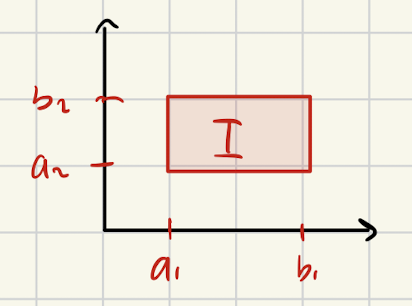
\includegraphics[width= 100pt, center]{K.png}
	
	\begin{theorem} (Nested Cell Property)
		If $I_1 \supseteq I_2 \supseteq I_3 \supseteq ...$ is a nested sequence of k-cells, then $\bigcap \limits_{n=1}^\infty I_n \not = \emptyset$.
	\end{theorem}
	\begin{proof}
		For each $n\in \N$, let
		$$I_n = [a_1 ^{(1)}, b_1 ^{(1)}] \times ... \times [a_k ^{(k)}, b_k ^{(k)}].$$
		Also, let
		$$ \forall n \in \N ~~\forall 1 \leq i \leq k ~~A_i ^{(i)} = [a_i ^{(n)}, b_i^{(n)}].$$
		So, 
		$$ \forall n \in \N ~~I_n = A_1^{(n)} \times ... \times A_k ^{(n)}.$$
		Since for each $n \in \N$, $I_n \supseteq I_{n+1},$ we have
		$$\forall 1 \leq i \leq k ~~ A_i ^{(n)} \supseteq A_i^{(n+1)}$$
		That is,
		\begin{align*}
			I_1 &= A_1^{(1)} \times ... \times A_k ^{(1)} \\
			I_2 &= A_2 ^{(2)} \times ... \times A_k^{(2)} \\
			\vdots \\
			I_n &= A_n^{(1)} \times ... \times A_n^{(n)} \\
			\vdots
		\end{align*}
		Hence, it follows from the nested interval property that
		$$\exists x_1 \in \bigcap \limits_{n=1}^\infty A_1^{(n)}, \exists x_2 \in \bigcap \limits_{n=1}^\infty A_2^{(n)}, ... \exists x_k \in \bigcap \limits{n=1}^{\infty} A_k ^{(n)}$$
		Thus,
		\begin{align*}
			(x_1,...,x_n) &\in \left[\bigcap \limits_{n=1}^\infty A_1^{(n)}\right] \times \left[\bigcap \limits_{n=1}^\infty A_2^{(n)}\right] \times... \times \left[\bigcap \limits_{n=1}^\infty A_k^{(n)}\right] \\
			&\subseteq \bigcap \limits_{n=1}^\infty \left[A_1^{(1)} \times ... \times A_k^{(n)}\right] \\
			&= \bigcap \limits_{n=1}^\infty I_n
		\end{align*}
		So, $\bigcap \limits_{n=1}^\infty I_n \not = \emptyset.$ \qed
	\end{proof}
	
	\begin{theorem}
		Every k-cell in $\R ^k$ is compact.
	\end{theorem}

	\begin{proof}
		Here we will prove the claim for 2-cells. The proof for a general k-cell is completely analogous.
		Let $I = [a_1,b_1] \times [a_2,b_2]$ be a 2-cell. Let $\varrow{a}=(a_1,a_2)$ and $\varrow{b}=(b_1,b_2)$.
		Let $\delta = d(\varrow{a}, \varrow{b})= ||\varrow{a} - \varrow{b}||_2 = sqrt{(a_1-b_1)^2+(a_2-b_2)^2}.$
		Noe that if $\varrow{x}=(x_1,x_2)$ and $\varrow{y}=(y_1,y_2)$ are any two points in I, then
		$$\begin{cases}
			x_1,y_1 \in [a_1,b_1] &\implies |x_1 - y_1| \leq |b_1 - a_1| \\
			x_2,y_2 \in [a_2,b_2] &\implies |x_2 - y_2| \leq |b_2 - a_2| \\
		\end{cases}
		\implies \sqrt{|x_1-y_1|^2+|x_2-y_2|^2} \leq \sqrt{|a_1-b_1|^2+|a_2-b_2|^2} = \delta$$
		So, $$d(\varrow{x}, \varrow{y}) \leq \delta.$$
		Let's assume for contradiction that $I$ is not compact. So, there exists an open cover $\ocover{G}$ of $I$ that does not have a finite subcover.
		For each $1 \leq i \leq 2$, divide $[a_i, b_i]$ into two subintervals of equal length:
		$$c_i= \frac{a_i + b_i}{2}, ~~ [a_i,b_i]=[a_i, c_i] \cup [c_i, b_i]$$
		These subintervals determine four 2-cells. There is at least one of these four 2-cells that is not covered by any finite subcollection of $\ocover{G}$.
		Let's call it $I_1$. Notice that
		$$\forall \varrow{x}, \varrow{y} \in I_1 ~~ ||\varrow{x}, \varrow{y}||_2 \leq \frac{\delta}{2}.$$
		Now, subdivide $I_1$ into four 2-cells and continue this process. We will obtain a sequence of 2-cells
		$$I_1, I_2, I_3, ... $$
		such that
		\begin{align*}
			&(i) I \supseteq I_1 \supseteq I_2 \supseteq ... \\
			&(ii) \forall \varrow{x}, \varrow{y} \in I_n ~~ ||\varrow{x}-\varrow{y}|| \leq \frac{\delta}{2^n} \\
			&(iii) \forall n \in \N, I_n \text{ cannot be covered by a finite subcollection of } \ocover{G}.
		\end{align*}
		By the nested cell property,
		$$\exists \varrow{x}^* \in I\cap I_1 \cap I_2 \cap...$$
		In particular,
		$$\varrow{x}^* \in I \subseteq \ocover{G} \implies \exists \alpha_0 \st \varrow{x}^* \in G_{\alpha_0}$$
		We have
		$$\begin{rcases}
			\varrow{x}^* \in G_{\alpha_0} \\
			G_{\alpha_0} \text{ is open}
		\end{rcases}
		\implies \exists r > 0 \st N_r(\varrow{x}^*) \subseteq G_{\alpha_0}$$
		Choose $n\in \N \st \frac{\delta}{2^n} < r.$ We claim that $I_n \in \nbhd{r}{\varrow{x}^*}.$ Indeed,
		suppose $\varrow{y}\in I_n$, we have $$\begin{cases}
			\varrow{y}\in I_n \\
			\varrow{x}^* \in I_n
		\end{cases}$$
		so $||\varrow{y} - \varrow{x}|| \leq \frac{\delta}{2^n} < r.$ Hence $\varrow{y} \in \nbhd{r}{\varrow{x}^*}.$ We have
		$$\begin{rcases}
			I_n \subseteq \nbhd{r}{\varrow{x}^*} \\
			\nbhd{r}{\varrow{x}^*} \subseteq G_{\alpha_0}
		\end{rcases}
		\implies I_n \subseteq G_{\alpha_0}$$
		This contradicts $(iii)$. \qed
	\end{proof}
\end{document}
\newpage

\section{Separated Sets, Disconnected Sets, and Connected Sets}
\graphicspath{{./images/}}
\begin{definition}[Separated, Disconnected, Connected]
    \routineMS.
    \begin{enumerate}[$(i)$]
        \item Two sets $A,B \subseteq X$ are said to be disjoint if $A\cap B = \emptyset$.
        \item Two sets $A,B \subseteq X$ are said to be separated if $\overline{A}\cap B = \emptyset = A \cap \overline{B}$.
        \item A set $E\subseteq X$ is said to be disconnected if it can be written as a union of two nonempty separated sets $A$ and $B$ $(E=A\cup B)$.
        \item A set $E\subseteq X$ is said to be connected if it is not disconnected.
    \end{enumerate}
\end{definition}

\begin{example}
    Consider $\R$ with the standard metric.
    \begin{enumerate}[$*)$]
        \item $A=(1,2)$ and $B=(2,5)$ are serparated.
        \begin{align*}
            &\overline{A}\cap B = [1,2] \cap (2,5) = \emptyset \\
            &A\cap \overline{B} = (1,2) \cap [2,5] = \emptyset \\
            &\implies E=A\cup B \text{ is disconnected.}
        \end{align*}

        \item $C = (1,2]$ and $D-(2,5)$ are disjoint but not separated.
        \begin{align*}
            &C \cap \overline{D} = (1,2] \cap [2,5] = \{2\} \\
            &C \cup D = (1,5) \text{ is indeed connected.}
        \end{align*}
    \end{enumerate}
\end{example}

\begin{theorem}
    \label{thm2.47}
    The following are equivalent:
    \begin{enumerate}[$(i)$]
        \item A nonempty subset of $\R$ is connected $\iff$ it is a singleton or an interval.
        \item Let $E\subseteq \R$. $E$ is connected $\iff$ if $x,y\in E$ and $x < z < y$, then $z\in E$.
    \end{enumerate}
\end{theorem}
\begin{proof}
    HW 6 \qed
\end{proof}
So, in $\R$, connected $\iff$ interval $\iff$ path connected.

\begin{definition}[Perfect Set]
    \routineMS and let $E\subseteq X.$.
    \begin{enumerate}[$(i)$]
        \item $E$ is said to be perfect if $E' = E$.
        \item $E$ is said to be perfeect if $E' \subseteq E$ and $E\subseteq E'$.
        \item $E$ is said to be perfect if $E$ is closed and every point of $E$ is a limit point.
        \item $E$ is said to be perfect if $E$ is closed and $E$ does not have isolated points.
    \end{enumerate}
\end{definition}

\begin{example} \leavevmode \\
    \begin{enumerate}[$*)$]
        \item $E=[0,1] \implies E' = [0,1]$, so $E=E' \implies E$ is perfect.
        \item $E=[0,1]\cup \{2\} \implies 2$ is an isolated point of $E \implies E$ is not perfect.
        \item $E=\{\frac{1}{n} : n\in \N\} \implies E' = {0}$ so $E \not = E',$ so $E$ is not perfect. Is $E'$ perfect?
        $$E' = {0} \implies (E')' = \emptyset, \text{ so $E'$ is not perfect.}$$
    \end{enumerate}
\end{example}

\begin{theorem}
    \label{thm2.43}
    Let $P$ be a nonempty perfect set in $\R^k$. Then $P$ is uncountable. (An exmaple of an immediate consequence: $[0,1]$ is uncountable)
\end{theorem}
\begin{proof}
    In our proof, we will use the following Lemmas:
    \begin{lemma}
        \label{lemma1}
        \routineMS and let $E\subseteq X$ be perfect. If $V$ is any open set in $X$ \st $V\cap E \not = \emptyset$, then $V\cap E$ is an infinite set.
    \end{lemma}
    \begin{proof}
        Let $q\in V\cap E.$ Then
        \begin{equation*}
            \begin{cases*}
                q \in V \implies \exists \delta > 0 \st \nbhd{\delta}{a} \subseteq V \\
                q \in E \implies q \in E'
            \end{cases*}
            \tag{$1$}
        \end{equation*}
        \begin{equation*}
            q \in E' \implies \nbhd{\delta}{q}\cap E \text{ is an infinite set.}
            \tag{$2$}
        \end{equation*}
        $(1),(2) \implies V\cap E$ is infinite.\qed
    \end{proof}

    \begin{lemma}
        \label{lemma2}
        Let $q\in \R^k$. Let $r > 0.$ Then
        $$\overline{\nbhd{r}{q}}=\overline{\{z\in \R^k : \|z-q\|_2 < r\}} = \{z\in \R^k : \|z-q\|_2 \leq r\} = C_r(q).$$
    \end{lemma}
    \begin{proof}
        HW 6 \qed
    \end{proof}

    Notice that
    $$
    \begin{rcases*}
        P' = P \\
        P \not = \emptyset
    \end{rcases*}
    \implies P' \not = \emptyset \implies P \text{ is infinite.}
    $$
    Assume for contradiction $P$ is countable. Let's denote the distinct elements of $P$ by $x_1, x_2, x_3,... :$
    $$P=\{x_1, x_2, x_3,...\}$$
    In what follows, we will construct a sequence of neighborhoods $V_1, V_2, V_3,... \st$
    \begin{enumerate}[$(i)$]
        \item $\forall n \in \N ~~\overline{V} \subseteq V_n$
        \item $\forall n \in \N ~~x_n \not \in \overline{V_{n+1}}$
        \item $\forall n \in \N ~~V_n \cap P \not \in \emptyset$
    \end{enumerate}
    First, let's assume we have constructed these neighborhoods.
    Then for each $n\in\N$, let
    $$K_n = \overline{V_n} \cap P \not = \emptyset$$
    Note that
    \begin{enumerate}[$(I)$]
        \item $\overline{V_{n+1}} \subseteq V_n \subseteq \overline{V_n}$ so $\overline{V_{n+1}}\cap P \subseteq \overline{V_n} \cap P \implies K_{n+1} \subseteq K_n$ for each $n.$
        \item $\begin{rcases*}
            \overline{V} \text{ is a closed and bounded set in $\R^k \implies \overline{V_n}$ is compact.} \\
            P \text{ is perfect $\implies P$ is closed.}
        \end{rcases*} \implies K_n = \overline{V_n}\cap P \text{ is compact.}$
    \end{enumerate}
    \begin{equation*}
        (I),(II) \overset{Thm 2.36}{\implies} \bigcap \limits_{n=1}^\infty K_n \not = \emptyset
        \tag{$*$}
    \end{equation*}
    Recall that $\forall n, K_n \subseteq P,$ so
    $$\bigcap \limits_{n=1}^\infty K_n \subseteq P$$
    However, if $b\in P$ then $b \not \in \bigcap \limits_{n=1}^\infty K_n$; indeed
    $$b\in P \implies b=x_m \text{ for some $m\in \N$}$$
    But $x_m \not \in \overline{V_{m+1}}$ so $x_m \not \in \overline{V_{m+1}\cap P} = K_{m+1}.$ So $x_m \not \in \bigcap \limits_{n=1}^\infty K_n.$ This tells us
    \begin{equation*}
        \bigcap \limits_{n=1}^\infty K_n = \emptyset
        \tag{$**$}
    \end{equation*}
    $$(*),(**) \implies \text{contradiction.}$$

    It remains to show that there exists a seequence of neighborhoods $V_1, V_2, V_3, ...$ satisfying $(i),(ii),(iii)$. We construct these sequences inductively.

    \begin{description}
        \item[Step 1:] Fix $r_1 > 0.$ Let $V_1 = \nbhd{r_1}{x_1}.$ Clearly, $V_1 \cap P \not = \emptyset$.
        \item[Step 2:] Our goal is to construct a neighborhood $V_2 \st$
        \begin{enumerate}[$(i)$]
            \item $\overline{V_2} \subseteq V_1$
            \item $x_1 \not \in V_2$
            \item $V_2 \cap P \not = \emptyset$
        \end{enumerate}
        We can do this just by using the fact that $V_1 \cap P \not = \emptyset.$.
        \begin{align*}
            V_1 \cap P \not = \emptyset \overset{\text{lem\ref{lemma1}}}{\implies} \exists y_1 \in V_1 \cap P \st y_1 \not = x_1 \\
            y_1 \in V_1 \overset{V \text{ is open}}{\implies} \exists \delta_1 > 0 \st \nbhd{\delta_1}{y_1} \subseteq V_1.
        \end{align*}
        Let $r_2 = \frac{1}{2} \min\{d(x_1,y_1), \delta_1\}.$ Let $V_2 = \nbhd{r_2}{y_1}.$ We claim $V_2$ has all the desired properties. Indeed,
        \begin{enumerate}[$(i)$]
            \item $\begin{aligned}[t]
                \overline{V_2} = \overline{\nbhd{r_2}{y_1}} &= \{z \in \R^k : \|z-y_1\|_2 \leq r_2\} \\
                &\subseteq \{z\in \R^k : \|z-y_1\|_2 < \delta_1\} = \nbhd{\delta_1}{y_1} \text{ since $r_2 < \delta_1$}\\
                &\subseteq V_1
            \end{aligned}$
            \item$d(x_1, y_1) > r_2 \implies x_1 \not \in \overline{\nbhd{r_2}{y_1}} = \{z\in \R^k : \|z-y_1\|_2 \leq r_2\}$
            \item $y_1 \in V_2$ and $y_1 \in P \implies V_2 \cap P \not = \emptyset$
        \end{enumerate}

        \item[Step 3:] Repeat the process to find $V_3$:
        \begin{enumerate}[$(i)$]
            \item $\closure{V_3} \subseteq V_2$
            \item $x_2 \not \in \closure{V_3}$
            \item $V_3 \cap P \not = \emptyset$
        \end{enumerate}
        Similarly, for each $k \geq 3,$ we can construct $V_{k+1}$ using only the fact that $V_k \cap P \not = \emptyset.$
    \end{description}
    \qed
\end{proof}

Consider the following construction:
\begin{description}
    \item[\underline{Stage 0:}]\leavevmode \\
    Let $E_0 = [0,1]$.
\end{description}

\begin{figure}[h]
    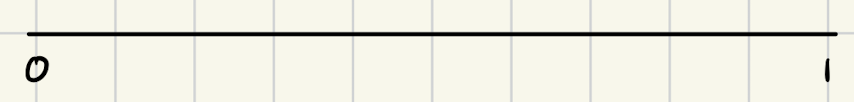
\includegraphics[width=.50\linewidth, center]{/Users/josiahvillarante/GradSchool/Grad-School-Notes/Math230A/Lecture/CH2/images/cantor set 0.png}
\end{figure}

\begin{description}
    \item[\underline{Stage 1:}]\leavevmode \\
    Remove the segment $(\frac{1}{3}, \frac{2}{3})$. That is, remove the middle third of the interval, and define $E_1 = [0, \frac{1}{3}]\cup [\frac{2}{3}, 1]$.
\end{description}

\begin{figure}[h]
    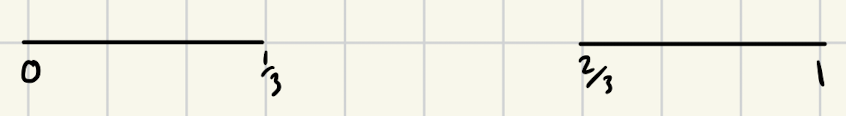
\includegraphics[width=.50\linewidth, center]{/Users/josiahvillarante/GradSchool/Grad-School-Notes/Math230A/Lecture/CH2/images/cantor set 1.png}
\end{figure}

\begin{description}
    \item[\underline{Stage 2:}]\leavevmode \\
    Take each of the intervals $[0, \frac{1}{3}]$ and $[\frac{2}{3}, 1]$ and remove the middle third of each those, and define $$E_2=\left[0, \frac{1}{9}\right]\cup \left[\frac{2}{9}, \frac{3}{9}\right] \cup \left[\frac{6}{9}, \frac{7}{9}\right] \cup \left[\frac{8}{9}, 1\right]$$.
\end{description}

\begin{figure}[h]
    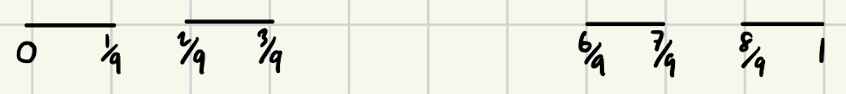
\includegraphics[width=.50\linewidth, center]{/Users/josiahvillarante/GradSchool/Grad-School-Notes/Math230A/Lecture/CH2/images/cantor set 2.png}
\end{figure}

Continuing this process, we will obtain a sequence of compact sets:
$$E_1, E_2, E_3,...$$
\st
\begin{enumerate}
    \item $E_1 \supseteq E_2 \supseteq E_3 \supseteq ...$
    \item For each $n \in \N, ~E_n$ is the union of $2^n$ intervals of length $\frac{1}{3^n}$.
\end{enumerate}

\begin{definition}[The Cantor Set]
    The Cantor set is the set
    $$P= \bigcap \limits_{n=1}^\infty E_n$$
    where each $E_n$ is defined from above.
\end{definition}

\begin{observation}
    Notice that in order to obtain $E_n$, we remove intervals of the form $(\frac{3k+1}{3^n}, \frac{3k+2}{3^n})$.
\end{observation}

\begin{theorem}[Properties of the Cantor set]
Let $P$ denote the Cantor set. Then
\begin{enumerate}[$(i)$]
    \item $P$ is compact
    \item $P$ is nonempty
    \item $P$ contains no segment
    \item $P$ is perfect (and so uncountable)
    \item $P$ has measure zero
\end{enumerate}    
\end{theorem}
\begin{proof}
    \begin{enumerate}[$(i)$]
        \item $P$ is an intersection of compact sets
        \item By Theorem \ref{thm2.36}, the intersection of a sequence of nested, nonempty, compact sets is nonempty
        \item Our goal is to show that $P$ does not contain any set of the form $(\alpha, \beta)$ (where $0 \leq \alpha, ~\beta \leq 1$). Note that, by construction of $P$, the intervals of the form 
        $$I_{k,n} = (\frac{3k+1}{3^n}, \frac{3k+2}{3^n}) ~~n\in\N, ~0\leq k \st 3k+2 < 3^n$$
        have no intersection with $P$.
        However, $(\alpha, \beta)$ contains at least one of $I_{k,n}$'s. Indeed,
        \begin{align*}
            &(\alpha, \beta) \text{ contains $(\frac{3k+1}{3^n}, \frac{3k+2}{3^n})$} \\
            &\iff \alpha < \frac{3k+1}{3^n} \text{ and } \frac{3k+2}{3^n} < \beta \\
            &\iff \frac{3^n \alpha - 1}{3} < k < \frac{3^n \beta - 2}{3}.
        \end{align*}
        So, to ensure $(\alpha, \beta)$ contains aty least one of $I_{k,n}$, it is enough to choose $n\in \N$ \st
        \begin{enumerate}[$(1)$]
            \item $(\frac{3^n\beta - 2}{3}) - (\frac{3^n \alpha -1}{3}) > 1$
            \item $\frac{3^n\beta - 2}{3} > 1$
        \end{enumerate}
        We have
        \begin{enumerate}[$(1)$]
            \item $\iff \frac{3^n(\beta - \alpha) -1}{3} > 4 \iff 3^n (\beta - \alpha) > 4 \iff 3^{-n} < \frac{\beta - \alpha}{4}$
            \item $\iff 3^n \beta - 2 > 3 \iff 3^n \beta > 5 \iff 3^{-n} < \frac{\beta}{5}$
        \end{enumerate}
        So, if we choose $n\in\N \st \frac{1}{3^n} < \min\{\frac{\beta - \alpha}{4}, \frac{\beta}{5}\}$, then we can be sure that $(\alpha, \beta)$ contains $I_{k,n}$ for some positive integer $k$.
        \item $P$ is perfect. We know that $P$ is closed (because it's an intersection of closed sets). So, in order to prove that $P$ is perfect, it is enough to show that every point of $P$ is a limit point of $P$. Let $x\in P$. We want to show $x \in P'$. That is,
        $$\forall \epsilon > 0 ~~\nbhd{\epsilon}{x} \cap (P \backslash \{x\})\not =\emptyset.$$
        We have
        $$x\in P = \bigcap \limits_{n=1}^\infty E_n \implies\forall n \in \N ~x \in E_n \implies \forall n \in \N ~~\exists I_n \subseteq E_n \st x\in I_n.$$
        Choose $n$ large enough \st $|I_n| < \frac{\epsilon}{2}.$ We have
        $$x \in I_n \text{ and $|I_n| < \frac{\epsilon}{2}$} \implies I_n \subseteq (x-\epsilon, x+\epsilon).$$
        At least one of these endpoints of $I_n$ is not $x$, let's call it $y$. Then 
        $$y\in P, ~y\not = x, ~y\in I_n \subseteq(x-\epsilon, x+\epsilon).$$
        So,
        $$y\in (x-\epsilon, x+\epsilon) \cap (P \backslash \{x\}).$$
        Therefore,
        $$(x-\epsilon, x+\epsilon) \cap (P \backslash \{x\}) \not = \emptyset.$$
    \end{enumerate}
    \qed
\end{proof}
\newpage

\chapter{Numerical Sequences and Series}
\section{Sequences and Convergence}
\documentclass[a4paper]{article}
%\documentclass{tuftebook}
\usepackage{amsthm}
\usepackage[many]{tcolorbox}

\makeatletter

\makeatletter

\def\renewtheorem#1{%
	\expandafter\let\csname#1\endcsname\relax
	\expandafter\let\csname c@#1\endcsname\relax
	\gdef\renewtheorem@envname{#1}
	\renewtheorem@secpar
}
\def\renewtheorem@secpar{\@ifnextchar[{\renewtheorem@numberedlike}{\renewtheorem@nonumberedlike}}
\def\renewtheorem@numberedlike[#1]#2{\newtheorem{\renewtheorem@envname}[#1]{#2}}
\def\renewtheorem@nonumberedlike#1{
	\def\renewtheorem@caption{#1}
	\edef\renewtheorem@nowithin{\noexpand\newtheorem{\renewtheorem@envname}{\renewtheorem@caption}}
	\renewtheorem@thirdpar
}
\def\renewtheorem@thirdpar{\@ifnextchar[{\renewtheorem@within}{\renewtheorem@nowithin}}
\def\renewtheorem@within[#1]{\renewtheorem@nowithin[#1]}

\makeatother

%%%%%%%%%%%%%%%%%%%%
% New environments %
%%%%%%%%%%%%%%%%%%%%

\makeatother
%\mdfsetup{skipabove=1em,skipbelow=0em}

\tcbuselibrary{skins}

% Color definitions

\definecolor{proofcolor}{RGB}{0,0,0}

% Dark orange and Dark Red rgb
\definecolor{theorembordercolor}{RGB}{151, 63, 5}
\definecolor{theorembackgroundcolor}{RGB}{248, 241, 234}

\definecolor{examplebordercolor}{RGB}{0, 110, 184}
\definecolor{examplebackgroundcolor}{RGB}{240, 244, 250}

\definecolor{definitionbordercolor}{RGB}{0, 150, 85}
\definecolor{definitionbackgroundcolor}{RGB}{239, 247, 243}

\definecolor{propertybordercolor}{RGB}{128, 0, 128}
\definecolor{propertybackgroundcolor}{RGB}{255, 240, 255}

\definecolor{formulabordercolor}{RGB}{0, 0, 0}
\definecolor{formulabackgroundcolor}{RGB}{230, 229, 245}

\newtheoremstyle{theorem}
{0pt}{0pt}{\normalfont}{0pt}
{}{\;}{0.25em}
{{\sffamily\bfseries\color{theorembordercolor}\thmname{#1}~\thmnumber{\textup{#2}}.}
	\thmnote{\normalfont\color{black}~(#3)}}

\newtheoremstyle{definition}
{0pt}{0pt}{\normalfont}{0pt}
{}{\;}{0.25em}
{{\sffamily\bfseries\color{definitionbordercolor}\thmname{#1}~\thmnumber{\textup{#2}}.}
	\thmnote{\normalfont\color{black}~(#3)}}

\newtheoremstyle{example}
{0pt}{0pt}{\normalfont}{0pt}
{}{\;}{0.25em}
{{\sffamily\bfseries\color{examplebordercolor}\thmname{#1}.}
	\thmnote{\normalfont\color{black}~(#3)}}

\newtheoremstyle{property}
{0pt}{0pt}{\normalfont}{0pt}
{}{\;}{0.25em}
{{\sffamily\bfseries\color{propertybordercolor}\thmname{#1}~\thmnumber{\textup{#2}}.}
	\thmnote{\normalfont\color{black}~(#3)}}

\newtheoremstyle{formula}
{0pt}{0pt}{\normalfont}{0pt}
{}{\;}{0.25em}
{{\sffamily\bfseries\color{formulabordercolor}\thmname{#1}~\thmnumber{\textup{#2}}.}
	\thmnote{\normalfont\color{black}~(#3)}}

%%%%%%%%%%%%%%%%%%%%%%%%
% Theorem Environments %
%%%%%%%%%%%%%%%%%%%%%%%%

\theoremstyle{theorem}

\newtheorem{theorem}{Theorem}
\newtheorem{postulate}{Postulate}
\newtheorem{conjecture}{Conjecture}
\newtheorem{corollary}{Corollary}
\newtheorem{lemma}{Lemma}
\newtheorem{conclusion}{Conclusion}

\tcolorboxenvironment{theorem}{
	enhanced jigsaw, pad at break*=1mm, breakable,
	left=4mm, right=4mm, top=1mm, bottom=1mm,
	colback=theorembackgroundcolor, boxrule=0pt, frame hidden,
	borderline west={0.5mm}{0mm}{theorembordercolor}, arc=.5mm
}
\tcolorboxenvironment{postulate}{
	enhanced jigsaw, pad at break*=1mm, breakable,
	left=4mm, right=4mm, top=1mm, bottom=1mm,
	colback=theorembackgroundcolor, boxrule=0pt, frame hidden,
	borderline west={0.5mm}{0mm}{theorembordercolor}, arc=.5mm
}
\tcolorboxenvironment{conjecture}{
	enhanced jigsaw, pad at break*=1mm, breakable,
	left=4mm, right=4mm, top=1mm, bottom=1mm,
	colback=theorembackgroundcolor, boxrule=0pt, frame hidden,
	borderline west={0.5mm}{0mm}{theorembordercolor}, arc=.5mm
}
\tcolorboxenvironment{corollary}{
	enhanced jigsaw, pad at break*=1mm, breakable,
	left=4mm, right=4mm, top=1mm, bottom=1mm,
	colback=theorembackgroundcolor, boxrule=0pt, frame hidden,
	borderline west={0.5mm}{0mm}{theorembordercolor}, arc=.5mm
}
\tcolorboxenvironment{lemma}{
	enhanced jigsaw, pad at break*=1mm, breakable,
	left=4mm, right=4mm, top=1mm, bottom=1mm,
	colback=theorembackgroundcolor, boxrule=0pt, frame hidden,
	borderline west={0.5mm}{0mm}{theorembordercolor}, arc=.5mm
}
\tcolorboxenvironment{conclusion}{
	enhanced jigsaw, pad at break*=1mm, breakable,
	left=4mm, right=4mm, top=1mm, bottom=1mm,
	colback=theorembackgroundcolor, boxrule=0pt, frame hidden,
	borderline west={0.5mm}{0mm}{theorembordercolor}, arc=.5mm
}

%%%%%%%%%%%%%%%%%%%%%%%%%%%
% Definition Environments %
%%%%%%%%%%%%%%%%%%%%%%%%%%%

\theoremstyle{definition}
\newtheorem{definition}{Definition}
\newtheorem{review}{Review}

\tcolorboxenvironment{definition}{
	enhanced jigsaw, pad at break*=1mm, breakable,
	left=4mm, right=4mm, top=1mm, bottom=1mm,
	colback=definitionbackgroundcolor, boxrule=0pt, frame hidden,
	borderline west={0.5mm}{0mm}{definitionbordercolor}, arc=.5mm
}
\tcolorboxenvironment{review}{
	enhanced jigsaw, pad at break*=1mm, breakable,
	left=4mm, right=4mm, top=1mm, bottom=1mm,
	colback=definitionbackgroundcolor, boxrule=0pt, frame hidden,
	borderline west={0.5mm}{0mm}{definitionbordercolor}, arc=.5mm
}


%%%%%%%%%%%%%%%%%%%%%%%%
% Example Environments %
%%%%%%%%%%%%%%%%%%%%%%%%

\theoremstyle{example}
\newtheorem*{example}{Example}
\newtheorem*{remark}{Remark}
\newtheorem*{note}{Note}

\tcolorboxenvironment{example}{
	enhanced jigsaw, pad at break*=1mm, breakable,
	left=4mm, right=4mm, top=1mm, bottom=1mm,
	colback=examplebackgroundcolor, boxrule=0pt, frame hidden,
	borderline west={0.5mm}{0mm}{examplebordercolor}, arc=.5mm
}
\tcolorboxenvironment{remark}{
	enhanced jigsaw, pad at break*=1mm, breakable,
	left=4mm, right=4mm, top=1mm, bottom=1mm,
	colback=white, boxrule=0pt, frame hidden,
	borderline west={0.5mm}{0mm}{examplebordercolor}, arc=.5mm
}
\tcolorboxenvironment{note}{
	enhanced jigsaw, pad at break*=1mm, breakable,
	left=4mm, right=4mm, top=1mm, bottom=1mm,
	colback=white, boxrule=0pt, frame hidden,
	borderline west={0.5mm}{0mm}{examplebordercolor}, arc=.5mm
}


%%%%%%%%%%%%%%%%%%%%%%%%%
% Property Environments %
%%%%%%%%%%%%%%%%%%%%%%%%%

\theoremstyle{property}
\newtheorem{property}{Property}
\newtheorem{proposition}{Proposition}

\tcolorboxenvironment{property}{
	enhanced jigsaw, pad at break*=1mm, breakable,
	left=4mm, right=4mm, top=1mm, bottom=1mm,
	colback=propertybackgroundcolor, boxrule=0pt, frame hidden,
	borderline west={0.5mm}{0mm}{propertybordercolor}, arc=.5mm
}
\tcolorboxenvironment{proposition}{
	enhanced jigsaw, pad at break*=1mm, breakable,
	left=4mm, right=4mm, top=1mm, bottom=1mm,
	colback=propertybackgroundcolor, boxrule=0pt, frame hidden,
	borderline west={0.5mm}{0mm}{propertybordercolor}, arc=.5mm
}

%%%%%%%%%%%%
% Formula %
%%%%%%%%%%%%

\theoremstyle{formula}
\newtheorem{formula}{Formula}

\tcolorboxenvironment{formula}{
	enhanced jigsaw, pad at break*=1mm, breakable,
	left=4mm, right=4mm, top=1mm, bottom=1mm,
	colback=formulabackgroundcolor, boxrule=0pt, frame hidden,
	borderline west={0.5mm}{0mm}{formulabordercolor}, arc=.5mm
}

%%%%%%%%%
% Proof %
%%%%%%%%%

% These patches must be placed after \tcolorboxenvironment !
\AddToHook{env/theorem/after}{\colorlet{proofcolor}{theorembordercolor}}
\AddToHook{env/postulate/after}{\colorlet{proofcolor}{theorembordercolor}}
\AddToHook{env/conjecture/after}{\colorlet{proofcolor}{theorembordercolor}}
\AddToHook{env/corollary/after}{\colorlet{proofcolor}{theorembordercolor}}
\AddToHook{env/lemma/after}{\colorlet{proofcolor}{theorembordercolor}}
\AddToHook{env/conclusion/after}{\colorlet{proofcolor}{theorembordercolor}}

\AddToHook{env/definition/after}{\colorlet{proofcolor}{definitionbordercolor}}
\AddToHook{env/review/after}{\colorlet{proofcolor}{definitionbordercolor}}

\AddToHook{env/example/after}{\colorlet{proofcolor}{examplebordercolor}}
\AddToHook{env/remark/after}{\colorlet{proofcolor}{examplebordercolor}}
\AddToHook{env/note/after}{\colorlet{proofcolor}{examplebordercolor}}

\AddToHook{env/property/after}{\colorlet{proofcolor}{propertybordercolor}}
\AddToHook{env/proposition/after}{\colorlet{proofcolor}{propertybordercolor}}

\AddToHook{env/formula/after}{\colorlet{proofcolor}{formulabordercolor}}

\renewcommand{\qedsymbol}{Q.E.D.}
\let\qedsymbolMyOriginal\qedsymbol
\renewcommand{\qedsymbol}{
	\color{proofcolor}\qedsymbolMyOriginal
}

\newtheoremstyle{proof}
{0pt}{0pt}{\normalfont}{0pt}
{}{\;}{0.25em}
{{\sffamily\bfseries\color{proofcolor}\thmname{#1}.}
	\thmnote{\normalfont\color{black}~(\textit{#3})}}

\theoremstyle{proof}
\renewtheorem{proof}{Proof}

\tcolorboxenvironment{proof}{
	enhanced jigsaw, pad at break*=1mm, breakable,
	left=4mm, right=4mm, top=1mm, bottom=1mm,
	colback=white, boxrule=0pt, frame hidden,
	borderline west={0.5mm}{0mm}{proofcolor}, arc=.5mm
}

\newenvironment{info}{\begin{tcolorbox}[
		arc=0mm,
		colback=white,
		colframe=gray,
		title=Info,
		fonttitle=\sffamily,
		breakable
		]}{\end{tcolorbox}}
\newenvironment{terminology}{\begin{tcolorbox}[
		arc=0mm,
		colback=white,
		colframe=green!60!black,
		title=Terminology,
		fonttitle=\sffamily,
		breakable
		]}{\end{tcolorbox}}
\newenvironment{warning}{\begin{tcolorbox}[
		arc=0mm,
		colback=white,
		colframe=red,
		title=Warning,
		fonttitle=\sffamily,
		breakable
		]}{\end{tcolorbox}}
\newenvironment{caution}{\begin{tcolorbox}[
		arc=0mm,
		colback=white,
		colframe=yellow,
		title=Caution,
		fonttitle=\sffamily,
		breakable
		]}{\end{tcolorbox}}

\date{}
\title{\flushleft \textbf{Sequences and Convergence}}
\begin{document}
    \maketitle

    \begin{definition} (Convergence of a Sequence)
        \routineMS and let $(x_n)$ be a sequence in $X$.
        $(x_n)$ converges to a limit $x\in X$ if and only if for every $\epsilon > 0$, we
        can find $N \in \N \st$ if $n > N, ~~ d(x_n, x) < \epsilon.$
    \end{definition}
    \begin{notation} $\\$
        \begin{enumerate}
            \item $x_n \rightarrow x$ as $n\rightarrow \infty$
            \item $x_n \rightarrow x$
            \item $\lim_{x\to\infty} x_n = x$
        \end{enumerate}
    \end{notation}

    \begin{remark}
        \begin{enumerate}[(i)]
            \item $x_n \to x \iff \forall \epsilon > 0 ~~ \exists N \in \Z \st \forall n > N ~~ d(x_n,x) < \epsilon.$
            \item If $(x_n)$ does not converge, we say it diverges.
            \item $x_n \to x \iff \forall \epsilon > 0 ~~ \exists N \in \Z \st \forall n > N ~~d(x_n, x) < \epsilon \\ x_n \to x \iff \forall \epsilon > 0 ~~ \exists N \in \R \st \forall n > N ~~d(x_n, x) < \epsilon$
        \end{enumerate}
    \end{remark}

    \begin{definition} (Bounded Sequence)
        \routineMS and let $(x_n)$ be a seqence in $X$. $(x_n)$ is said to be bounded if the set $\{x_n : n \in \N\}$ is a bounded set in the metric space $X$.
        \begin{align*}
        (x_n) \text{ is bounded } &\iff \exists q\in X ~\exists r > 0 \st \{x_n : n \in \N\} \subseteq \nbhd{r}{q} \\ &\iff \exists q \in X ~\exists r > 0 \st d(x,q) < r
        \end{align*}
    \end{definition}

    \begin{example}
        Consider $\R$ equipped with the standard metric.
        \begin{enumerate}[(i)]
            \item $x_n = (-1)^n:$ this sequence is bounded, has a finite range $\{-1, 1\}$, and diverges.
            \item $x_n = \frac{1}{n}:$ this sequence is bounded, has an infinite range, and converges to $0$.
            \item $x_n = 1:$ this sequence is bounded, has a finite range, and converges to 1.
            \item $x_n=n^2:$ this sequence is undbounded, has an infinite range, and diverges.
        \end{enumerate}
    \end{example}

    \begin{example}
        Consider $Y= (0, \infty)$ with the induced metric from $\R$.
        $x_n = \frac{1}{n}:$ this sequence is bounded, has infinite range, and diverges.
    \end{example}

    \begin{theorem}(An equivalent characterization of convergence)
        \routineMS.
        $$x_n \to x \iff \forall \epsilon > 0 ~\nbhd{\epsilon}{x} \text{ contains $x_n$ for all but at most finitely many $n$.}$$
    \end{theorem}
    \begin{proof}
        \begin{align*}
            x_n \to x &\iff \forall \epsilon > 0 ~\exists N \in \N \st \forall n > N ~d(x_n, x) < \epsilon \\
            &\iff \forall \epsilon > 0 ~\exists N \in \N \st \forall n > N ~x_n \in \nbhd{\epsilon}{x} \\
            &\iff \forall \epsilon > 0 ~\exists N \in \N \st \nbhd{\epsilon}{x} \text{ contains } x_n ~\forall n > N \\
            &\iff \forall \epsilon > 0 ~\nbhd{\epsilon}{x} \text{ contains $x_n$ for all but at most finitely many $n$}.
        \end{align*}
    \end{proof}

    \begin{theorem}(Uniqueness of a Limit)
        \routineMS and let $(x_n)$ be a sequence in $X$. If $x_n \to x$ in $X$ and $x_n \to \overset{-}{x}$ in $X$, then $x = \overset{-}{x}$.
    \end{theorem}
     To prove this theorem, we make use of the following lemma:
     \begin{lemma}
        \label{lem 1}
        Suppose $a \geq 0.$ If $a < \epsilon ~\forall \epsilon > 0,$ then $a=0$.
     \end{lemma}
     \begin{proof}
        In order to prove that $x = \overset{-}{x},$ it is enough to show that $d(x, \overset{-}{x}) = 0.$ To this end, according to Lemma \ref{lem 1}, it is enough to show that
        $$\forall \epsilon > 0 ~ d(x, \overset{-}{x}) < epsilon.$$
        Let $\epsilon > 0$ be given.
        \begin{align*}
            x_n \to x &\implies \exists N_1 \st \forall n > N_1 ~d(x_n, x) < \frac{\epsilon}{2} \\
            x_n \to \overset{-}{x} &\implies \exists N_2 \st \forall n > N_2 ~d(x_n, \overset{-}{x}) < \frac{\epsilon}{2}
        \end{align*}
        Let $N= \max\{N_1, N_2\}$. Pick any $n > N$. We have
        \begin{align*}
            d(x, \overset{-}{x}) &\leq d(x, x_n) + d(x_n, \overset{-}{x}) \\
            &< \frac{\epsilon}{2} + \frac{\epsilon}{2} \\
            &= \epsilon.
        \end{align*}
        \qed
     \end{proof}

     \begin{theorem}(Convergent $\implies$ bounded)
        \routineMS and let $(x_n)$ be a sequence in $X$. If $x_n \to x$ in $X$, then $(x_n)$ is bounded.
     \end{theorem}
     \begin{proof}
        By definition of convergence with $\epsilon = 1$, we have
        $$\exists N \in \N \st \forall n > N ~x_n \in N_1(x).$$
        Now, let $r= \max \{1, d(x_1, x), d(x_2, x), ..., d(x_n, x)\} + 1$.
        Then, clearly,
        $$\forall n \in \N ~d(x_n, x) < r$$
        Hence,
        $$ \forall n \in \N ~x_n \in N_r(x).$$
        Therefore, $(x_n)$ is bounded. \qed
     \end{proof}

     \begin{corollary} (contrapositive)
        If $(x_n)$ is NOT bounded in $X$, then $(x_n)$ diverges in $X$.
     \end{corollary}

     \begin{theorem}(Limit Point is a Limit of a Sequence)
        \routineMS and let $E\subseteq X$. Suppose $x \in E'$. Then there exists a sequence $x_1, x_2, ...$ of distinct points in $E \backslash \{x\}$ that converges to $x$.
     \end{theorem}
     \begin{proof}
        Since $x\in E',$
        $$\forall \epsilon > 0 ~\nbhd{\epsilon}{x} \cap (E \backslash \{x\}) \text{ is infinite.}$$
        In particular,
        \begin{align*}
            &\text{for } \epsilon = 1 ~\exists x_1 \in E \backslash \{x\} \st d(x_1, x) < 1 \\
            &\text{for } \epsilon = \frac{1}{2} ~\exists x_2 \in E \backslash \{x\} \st x_2 \not = x_1 \wedge d(x_2, x) < \frac{1}{2} \\
            &\text{for } \epsilon = \frac{1}{3} ~\exists x_3 \in E \backslash \{x\} \st x_3 \not = x_2 \wedge d(x_3, x) < \frac{1}{3} \\
            \vdots \\
            &\text{for } \epsilon = \frac{1}{n} ~\exists x_n \in E \backslash \{x\} \st x_n \not = x_1, x_2, x_3,... \wedge d(x_n, x) < \frac{1}{n} \\
            \vdots
        \end{align*}
        In this way we obtain a sequence $x_1, x_2, x_3,...$ of distinct points in $E \backslash \{x\}$ that converges to $x$.
        Let $\epsilon > 0$ be given. We need to find $N$ such that if $n > N$ then $d(x_n, x) < \epsilon$. Let $N$ be such that $\frac{1}{N} < \epsilon$ (archimedean property). Then $\forall n > N ~d(x_n, n) < \frac{1}{n} < \frac{1}{N} < \epsilon$ as desired. \qed
     \end{proof}
\end{document}
\newpage

\section{Subsequences}
\begin{definition} (Subsequences)
    \routineSeq Let $n_1 < n_2 < n_3 < ...$ be a strictly increasing sequence of natural numbers. Then $(x_{n_1}, x_{n_2}, x_{n_3},...)$ is called a subsequence of $(x_1, x_2, x_3,...)$, and is denoted by $(x_{n_k})$, where $k \in \N$ indexes the subsequence.
\end{definition}

\begin{example}
    Let $(x_n) = (1, \frac{1}{2}, \frac{1}{3}, \frac{1}{4},...)$.
    \begin{enumerate}[(i)]
        \item $(1, \frac{1}{3}, \frac{1}{5}, \frac{1}{7},...)$ is a subsequence.
        \item $(\frac{1}{100}, \frac{1}{1000}, \frac{1}{10000},...)$ is a subsequence.
        \item $(1, \frac{1}{5}, \frac{1}{3}, \frac{1}{7}, \frac{1}{2},...)$ is not a subsequence (we do not have $n_1 < n_2 < n_3 <...$).
    \end{enumerate}
\end{example}
\begin{remark}
    Suppose $(x_{n_1}, x_{n_2}, x_{n_3},...)$ is a subsequence of $(x_1, x_2, x_3, ...)$. Notice that $n_i \in \N$ and $n_1 < n_2 < n_3 < ...$ so
    \begin{enumerate}[(i)]
        \item $n_1 \geq 1$
        \item For each $k \geq 2,$ there are at least $k-1$ natural numbers, namely $n_1,...,n_{k-1}$, strictly less than $n_k$, so $n_k \geq k$.
    \end{enumerate}
\end{remark}

\begin{theorem}
    \routineSeq If $\lim \limits_{n \to \infty} x_n = x$, then every subsequence of $(x_n)$ converges to $x$.
\end{theorem}
\begin{proof}
    Let \subseq{x} be a subsequence of \seq{x}. Our goal is to show that $\lim \limits_{k \to \infty} x_{n_k} = x.$ That is, we want to show
    $$\forall \epsilon > 0 ~\exists N \in \N \st \forall k > N ~d(x_{n_k}, x) < \epsilon.$$
    Let $\epsilon > 0$ be given. Our goal is to find $N$ \st
    \begin{equation}
        \text{if $k > N$, then $d(x_{n_k}, x) < \epsilon$}
        \tag{$I$}
    \end{equation}
    Since $x_n \to x$, we have
    \begin{equation}
        \exists \hat{N} \st \forall n > \hat{N} ~d(x_n, x) < \epsilon
        \tag{$II$}
    \end{equation}
    We claim that this $\hat{N}$ can be used as the $N$ we are looking for. Indeed, if we let $N=\hat{N}$, then if $k > N$ we can conclude that $n_k \geq k > N$ and so, by $(II)$
    $$d(x_{n_k},x) < \epsilon$$ \qed
\end{proof}

\begin{corollary} (contrapositive)
    \begin{enumerate}[(i)]
        \item If a subsequence of $(x_n)$ does not converge to $x$, then $(x_n)$ does not converge to $x$.
        \item If $(x_n)$ has a pair of subsequences converging to different limits, then $(x_n)$ does not converge.
    \end{enumerate}
\end{corollary}

\begin{example}
    Let $x_n = (-1)^n$ in $\R$.
    \begin{enumerate}
        \item The subsequence $(x_1, x_3, x_5,...) = (-1, -1, -1,...)$ converges to $-1.$
        \item The subsequence$(x_2, x_4, x_6,...) = (1, 1, 1, ...)$ converges to $1$.
    \end{enumerate}
    By (i) and (ii), $(x_n)$ does not converge.
\end{example}

\begin{theorem}
    \routineSeq The subsequential limits of $(x_n)$ form a closed set in $X$.
\end{theorem}
\begin{proof}
    Let $E=\{b \in X : b \text{ is a limit of a subsequence of } x_n\}.$ Our goal is to show that $E' \subseteq E$. To this end, we pick an arbitrary element $a \in E'$ and we will prove that $a \in E$. That is, we will show that there is a subsequence of $(x_n)$ that converges to $a$. We may consider two cases:
    \begin{description}
        \item[Case 1: $\forall n \in \N ~x_n = a$.]
        In this case, $(x_n)$ and any subsequence of $(x_n)$ converges to $a$. So $a \in E.$
        \item[Case 2: $\exists n_1 \in \N \st x_{n_1} \not = a.$] Let $\delta = d(a, x_{n_1}) > 0.$ Since $a \in E', \nbhd{\frac{\delta}{2^2}}{a}\cap(E \backslash \{a\}) \not = \emptyset.$ So,
        $$\exists b \in E \backslash \{a\} \st d(b, a) < \frac{\delta}{2^2}.$$
        Since $b\in E$, $b$ is a limit of a subsequence of $(x_n)$, so
        $$\exists n_2 > n_1 \st d(x_{n_2}, b) < \frac{\delta}{2^2}.$$
        Now note that
        $$d(x_{n_2}, a) \leq d(x_{n_2}, b) + d(b,a) < \frac{\delta}{2^2} + \frac{\delta}{2^2} = \frac{\delta}{2}.$$
        Since $a \in E'$, $\nbhd{\frac{\delta}{2^3}}{a} \cap (E \backslash \{a\}) \not = \emptyset.$ So,
        $$\exists b \in E \backslash \{a\} \st d(b,a) < \frac{\delta}{2^3}.$$
        Since $b \in E$, $b$ is a limit of a subsequence of $(x_n)$, so
        $$\exists n_3 > n_2 \st ~d(x_{n_3}, b) < \frac{\delta}{2^3}.$$
        Now note that
        $$d(x_{n_3}, a) \leq d(x_{n_3},b) + d(b, a) < \frac{\delta}{2^3} + \frac{\delta}{2^3} = \frac{\delta}{2^2}.$$
        In this way, we obtain a subsequence $x_{n_1}, x_{n_2}, x_{n_3},...$ of $(x_n)$ \st
        $$\forall k \geq 2 ~~d(x_{n_k}, a) < \frac{\delta}{2^{k-1}}$$
        so, clearly, $x_{n_k} \to a.$ Hence, $a \in E.$ \qed
    \end{description}
\end{proof}

\begin{theorem} (Compactness $\implies$ Sequential Compactness)
    \label{thm3.6a}
    Let $(X,d)$ be a compact metric space. Then every sequence in $X$ has a convergent subsequence.
\end{theorem}

\begin{proof}
    Let $(x_n)$ be a sequence in the compact metric space $X$. Let $E=\{x_1, x_2,...\}.$ If $E$ is infinite, then there exists $x\in X$ and $n_1< n_2 < n_3<...$ \st
    $$x_{n_1} = x_{n_2} = x_{n_3} = ... = x.$$
    Clearly, the subsequence $(x_{n_1}, x_{n_2},...)$ converges to $x$. If $E$ is infinite, then since $X$ is compact, by Theorem 2.37, $E$ has a limit point $x\in X$. Since $x\in E'$,
    $$\forall \epsilon > 0 ~\nbhd{\epsilon}{x} \cap (E \backslash \{x\}) \text{ is infinite.}$$
    In particular,
    \begin{align*}
        &\text{for $\epsilon = 1, ~\exists n_1 \in \N \st d(x_{n_1}, x) < 1$} \\
        &\text{for $\epsilon = 2, ~\exists n_2 \in \N \st d(x_{n_2}, x) < \frac{1}{2}$} \\
        &\text{for $\epsilon = 3, ~\exists n_3 \in \N \st d(x_{n_3}, x) < \frac{1}{3}$} \\
        &\vdots \\
        &\text{for $\epsilon = m, ~\exists n_m \in \N \st d(x_{n_m}, x) < \frac{1}{m}$} \\
        &\vdots
    \end{align*}
    In this way, we obtain a subsequence $x_{n_1}, x_{n_2}, x_{n_3},...$ of $(x_n)$ that converges to $x$. \qed
\end{proof}

\begin{corollary} (Bolzano-Weierstrass)
    Every bounded sequence in $\R ^k$ has a convergent subsequence.
\end{corollary}
\begin{proof}
    Let $(x_n)$ be a bounded sequence in $\R ^k$.

    $$\implies \exists q \in \R ^k \text{ and } r > 0 \st \{x_1, x_2, x_3,...\} \subseteq \nbhd{r}{q}.$$

    Note that $\nbhd{r}{q}$ is bounded and so $\overline{\nbhd{r}{q}}$ is closed and bounded. So, $\overline{\nbhd{q}{r}}$ is a compact subset of $\R ^k$. So,
    $\closure{\nbhd{q}{r}}$ is a compact metric space and $(x_n)$ is a sequence in $\closure{\nbhd{q}{r}}$. By Theorem \ref{thm3.6a}, there exists a subsequence $(x_{n_k})$ of $(x_n)$ that converges in the metric space $\closure{\nbhd{r}{q}}$. Since the distance function in $\closure{\nbhd{r}{q}}$ is the same as the distance function in $\R ^k$, we can conclude that $(x_{n_k})$ converges in $\R^k$ as well. \qed
\end{proof}

Recall:
$$x_n \to x \iff \forall \epsilon > 0 ~\exists N \st \forall n > N ~d(x_n, x) < \epsilon.$$
This is useful \textit{IF} we know that a sequence converges. How do we first determine that a sequence converges? Perhaps, given a sequence $(x_n)$, we can determine convergence by comparing two consecutive terms:
$$\text{If }\forall \epsilon > 0 ~\exists N \st d(x_{n+1}, x_n) < \epsilon, \text{ then the sequence converges.}$$
Unfortunately, this will not do. Consider $\R: x_n = \sqrt{n}$ diverges (it is unbounded) yet 
$$x_{n+1} - x_n = \sqrt{n+1} - \sqrt{n} = \frac{n+1 - n}{\sqrt{n+1}+\sqrt{n}} = \frac{1}{\sqrt{n+1}+\sqrt{n}} \to 0.$$
Cauchy proposed that instead of comparing the distance between two consecutive terms, we compare the distance between \textit{any} two terms after a certain index:
$$\text{If }\forall \epsilon > 0 ~\exists N \st \forall n,m > N ~d(x_m, d_n) < \epsilon, \text{ then the sequence converges.}$$

\begin{definition} (Cauchy Sequence)
    \routineMS A sequence $(x_n)$ in $X$ is said to be a Cauchy Sequence if
    $$\forall \epsilon > 0 ~\exists N \st ~\forall n,m > N ~d(x_m,x_n) < \epsilon.$$
\end{definition}

\begin{theorem}(Convergent $\implies$ Cauchy)
    \label{thm3.11a}
    \routineSeq Then
    $$(x_n) \text{ converges} \implies (x_n) \text{ is a Cauchy sequence}$$
\end{theorem}

\begin{proof}
    Assume there exists $x\in X$ \st $x_n \to x$. Our goal is to show that
    \begin{equation}
        \forall \epsilon > 0 ~\exists N \st \forall n, m > N ~d(x_n, x_m) < \epsilon \tag{$I$}
    \end{equation}
    \begin{info}
    We want to make $d(x_n, x_m)$ less than $\epsilon$ using the fact that $d(x_n, x)$ and $d(x_m, x)$ can be made as small as we like for large enough $m$ and $n$. It would be great if we could bound $d(x_n, x_m)$ with a combination of $d(x_n, x)$ and $d(x_m, x)$. Note that
    $$d(x_n,x_m) \leq d(x_n, x) + d(x, x_m)$$
    so it is enough to make each piece on the RHS less than $\epsilon / 2$
    \end{info}
    We have
    $$x_n \to x \implies \exists \hat{N} \st \forall n > \hat{N} ~d(x_n, x) < \epsilon / 2.$$
    We claim that this $\hat{N}$ can be used as the $N$ that we were looking for. Indeed, if we let $N=\hat{N}$, $(I)$ will hold because $\forall n,m > \hat{N}$,
    \begin{align*}
        d(x_m,x_n) &\leq d(x_m, x) + d(x, x_n) \\
        &< \epsilon / 2 + \epsilon / 2 \\
        &= \epsilon,
    \end{align*}
    as desired. \qed
\end{proof}

\begin{remark}
    The converse in general is not true. Eg, consider $\Q$ as a subspace of $\R$. In $\Q$, it is not true that every Cauchy sequence is convergent. For example, let $(q_n)$ be a sequence in $\Q$ \st $q_n \to \sqrt{2}.$
    \begin{align*}
        q_n \to \sqrt{2} \text{ in } \R &\implies (q_n) \text{ is convergent in $\R$} \\
        &\implies (q_n) \text{ is Cauchy in $\R$} \\
        &\implies (q_n) \text{ is Cauchy in $\Q$}
    \end{align*}
    but $(q_n)$ does not converge in $Q$.
\end{remark}
It is desirable to define a metric space in which Cauchy sequences imply convergence.

\begin{definition} (Complete Metric Space)
    A metric space in which every Cauchy sequence is convergent is called a complete metric space.
\end{definition}
\newpage

\section{Diameter of a Set}
\begin{definition} (Diameter of a Set)
    \routineMS and let $E$ be a nonempty subset in $X$. The diameter of $E$, denoted by $diamE$, is defined as follows:
    $$diamE = sup\{d(a,b) : a,b \in E\}$$
\end{definition}

\begin{remark}
    Note that if $\empty \not = A \subseteq B \subseteq X,$ then
    $$\{d(a,b) : a,b \in A\} \subseteq \{d(a,b) : a,b \in B \}.$$
    Hence,
    $$ sup\diam{A} \subseteq sup\diam{B}$$.
    That is,
    $$diamA \leq diamB.$$
\end{remark}

\begin{observation}
    Let $(x_n)$ be a sequence in $X$. $\forall n \in \N$ let $E_n = \{x_{n+1}, x_{n+2},...\}.$ Then
    $$(x_n) \text{ is Cauchy} \iff \lim_{n \to \infty}diamE_n = 0.$$
\end{observation}

\begin{proof}
    Note that
    \begin{align*}
        &E_1 = \{x_2, x_3, x_4,...\} \\
        &E_2 = \{x_3, x_4, x_5,...\} \\
        &E_3 = \{x_4, x_5, x_6,...\} \\
        \vdots
    \end{align*}
    Clearly, $E_1 \supseteq E_2 \supseteq E_3 \supseteq ...$, so 
    $$diamE_1 \supseteq diamE_2 \supseteq diamE_3 \supseteq ...$$

    ($\implies$) Supposed $(x_n)$ is Cauchy. Our goal is to show that
    $$\forall \epsilon > 0 ~\exists N \st \forall n > N ~|diamE_n - 0| < \epsilon.$$
    Let $\epsilon > 0$ be given. Our goal is to find a number $N$ such that if $n > N$, then $diamE_n < \epsilon ~(*).$ For the given $\epsilon > 0$, since $(x_n)$ is Cauchy, there exists $\hat{N}$ \st
    $$ \forall n,m > \hat{N} ~d(x_n, x_m) < \epsilon / 2.$$
    We claim that this $\hat{N}$ can be used as the $N$ that we were looking for. Indeed, if we let $N = \hat{N}$, then $(*)$ will hold becuase:
    $$E_{\hat{N}} = \{x_{\hat{N}+1}, x_{\hat{N}+2}, x_{\hat{N}+3}\}$$
    so $\forall a,b \in E_{\hat{N}} ~d(a,b) < \epsilon / 2.$ Then
    $$diamE_{\hat{N}} = sup\diam{E_{\hat{N}}} \leq \epsilon / 2 < \epsilon$$
    so if $n > \hat{N}$, then
    $$diamE_n \leq diamE_{\hat{N}} < \epsilon$$
    as desired.\newline
    ($\impliedby$) Suppose $\lim_{n\to \infty}diamE_n = 0.$ Our goal is to show that 
    $$\forall \epsilon > 0 ~\exists N \st \forall n,m > N ~d(x_m, x_n) < \epsilon.$$
    Let $\epsilon > 0$ be given. Our goal is to find a number $N$ \st
    \begin{equation}
        \text{if } n,m > N, \text{ then } d(x_n, x_m) < \epsilon.
        \tag{$*$}
    \end{equation}
    Since $\lim_{n \to \infty} diamE_N = 0,$ for this $\epsilon$, there exists $\hat{N}$ \st
    $$\forall n > \hat{N} ~diamE_n < \epsilon$$
    We claim that $N = \hat{N} + 1$ can be used as the $N$ that we were looking for. Indeed, if we let $N = \hat{N} + 1$, then $(*)$ will hold:
    $$\text{if } n,m > \hat{N} + 1, \text{ then } x_n, x_m \in E_{\hat{N}+1}$$
    and so
    $$d(x_m,x_n) \leq diamE_{\hat{N}+1} < \epsilon$$
    \qed
\end{proof}

\begin{theorem}(diam$\closure{E}$ = diam $E$)
    \label{thm3.10a}
    \routineMS and let $\emptyset \not = E \subseteq X$. Then
    $$\text{diam$\closure{E} =$ diam $E$}$$
\end{theorem}

\begin{proof}
    Note that since $E \subseteq \closure{E}$, we have diam$E \leq$diam$\closure{E}$. In what follows, we will prove that diam$\closure{E} \leq$diam$E$ by showing that
    $$\forall \epsilon > 0 ~\text{diam$\closure{E} \leq$ diam$E + \epsilon$}.$$
    Let $\epsilon > 0$ be given. Our goal is to show that
    $$\sup\{d(a,b): a,b \in \closure{E}\} \leq \text{diam$E + \epsilon$}.$$
    To this end, it is enough to show that diam$E + \epsilon$ is an upper bound for $\{d(a,b) : a,b \in \closure{E}\}$. Suppose $a,b\in \closure{E}$. We have
    \begin{align*}
        a\in \closure{E} &\implies \nbhd{\epsilon/2}{a} \cap E \not = \emptyset \implies \exists x \in E \st d(x,a) < \frac{\epsilon}{2} \\
        b\in \closure{E} &\implies \nbhd{\epsilon/2}{b} \cap E \not = \emptyset \implies \exists y \in E \st d(y,b) < \frac{\epsilon}{2}.
    \end{align*}
    Therefore,
    \begin{align*}
        d(a,b) &\leq d(a,x) + d(x,y) + d(y,b) \\
        & < \frac{\epsilon}{2} + d(x,y) + \frac{\epsilon}{2} \\
        &\leq \frac{\epsilon}{2} + \text{diam$E$} + \frac{\epsilon}{2} \\
        &= \epsilon + \text{diam$E$}
    \end{align*}
    \qed
\end{proof}

\begin{theorem}
    \label{thm3.10b}
    \routineMS and let $K_1 \supseteq K_2 \supseteq K_3 \supseteq...$ be a nested sequence of nonempty compact sets.
\end{theorem}

\begin{proof}
    Let $K = \bigcap \limits_{n=1}^\infty K_n.$ By Theorem 2.36, we know that $K\not = \emptyset.$ In order to show that $K$ has only one element, we suppose $a,b \in K$ and we will prove $a=b$. In order to show $a=b$, we will prove $d(a,b) = 0$ and to this end show
    $$\forall \epsilon > 0 ~d(a,b) < \epsilon.$$
    Let $\epsilon > 0$ be given. Since $\lim_{n\to \infty}$ diam$K_n = 0$, there exists $N$ \st
    $$\forall n > N ~\text{diam$K_n$} < \epsilon.$$
    In particular, diam$K_{N+1} < \epsilon$. Now we have
    $$
    \begin{rcases*}
        a \in \bigcap \limits_{n = 1}^\infty K_n &$\implies a \in K_{N+1}$ \\ b\in \bigcap \limits_{n = 1}^\infty K_n &$\implies b \in K_{N+1}$ 
    \end{rcases*}
    \implies d(a,b) \leq \text{diam$K_{N+1} < \epsilon$}$$
    \qed
\end{proof}

\begin{theorem}(Compact Space $\implies$ Complete Space)
    \label{thm3.11b}
    Any compact metric space is complete.
\end{theorem}

\begin{proof}
    Let $(X,d)$ be a compact metric space. Let $(x_n)$ be a Cauchy sequence in $X$. Our goal is to show that $(x_n)$ converges in $X$. For each $n \in \N$, let $E_n = \{x_{n+1}, x_{n+2}, x_{n+3},...\}.$ We know that
    \begin{enumerate}[(1)]
        \item $E_1 \supseteq E_2 \supseteq E_3 \supseteq ...$
        \item $(x_n)$ is Cauchy $\implies \lim_{n\to \infty} \text{diam$E_n$} = 0$
    \end{enumerate}
    It follows from (1) that
    \begin{equation*}
        \closure{E_1} \supseteq \closure{E_2} \supseteq \closure{E_3} \supseteq ...
        \tag{$I$}
    \end{equation*}
    Since closed subsets of a compact space are compact, $(I)$ is a nested sequence of nonempty compact sets. Since diam$E_n = $diam$\closure{E_n}$, it follows from $(2)$ that $\lim_{n\to \infty}$diam$\closure{E_n} = 0$. Hence, by Theorem \ref{thm3.10b}, $\bigcap \limits_{n=1}^\infty \closure{E_n}$ has exactly one point. Let's call this point "$a$":
    $$\bigcap \limits_{n=1}^\infty \closure{E_n} = \{a\}$$
    In what follows, we will prove that $\lim_{n\to \infty} x_n = a.$ To this end, it's enough to show that
    $$\forall \epsilon > 0 ~\exists N \st \forall n > N ~d(a_n, a) < \epsilon.$$
    Let $\epsilon > 0$ be given. Our goal is to find $N$ \st
    \begin{equation*}
        \text{if $n > N,$ then $d(x_n,a) < \epsilon$}
        \tag{$*$}
    \end{equation*}
    Since $\lim_{n \to \infty}$diam$\closure{E} = 0$, for this given $\epsilon$ there exists $\hat{N}$ \st
    $$\forall n > \hat{N} ~\text{diam$\closure{E_n} < \epsilon$}.$$
    We claim that $\hat{N} + 1$ can be used as the $N$ that we are looking for. Indeed, if we let $N= \hat{N} + 1$, then $(*)$ holds:
    $$\text{If $n > \hat{N} + 1,$ then }
    \begin{rcases}
        x_n \in E_{\hat{N}+1} \implies x_n \in \closure{E_{\hat{N}+1}} \\
        a\in \bigcap \limits_{n=1}^\infty \closure{E_n}, \text{ so $a\in \closure{E_{\hat{N}+1}}$}
    \end{rcases}
    \implies d(x_n, a) \leq \text{diam$\closure{E_{\hat{N}+1}} < \epsilon$}
    $$
    \qed
\end{proof}

\begin{theorem}($\R^k$ is Complete)
    \label{thm3.11c}
    $\R^k$ is a complete metric space.
\end{theorem}
\begin{proof}
    Let $(x_n)$ be a Cauchy sequence in $\R^k$.
    \begin{align*}
        &\overset{\text{HW 7}}{\implies} (x_n) \text{ is bounded} \\
        &\implies \exists p \in \R^k, ~\epsilon > 0 \st \forall n \in \N ~x_n \in \nbhd{\epsilon}{p}.
    \end{align*}
    Note that $\closure{\nbhd{\epsilon}{p}}$ is closed and bounded in $\R^k$, so it's compact.
    $$
    \begin{rcases*}
        \closure{\nbhd{\epsilon}{p}} \text{ is a compact metric space } \\
        (x_n) \text{ is Cauchy in } \closure{\nbhd{\epsilon}{p}}
    \end{rcases*}
    \implies (x_n) \text{ converges to a point $x\in \closure{\nbhd{\epsilon}{p}}$}.
    $$
    Since the distance function in $\closure{\nbhd{\epsilon}{p}}$ is exactly the same as the distance function in $\R^k$, we can conclude that $x_n \to x$ in $\R^k$. \qed
\end{proof}
\newpage

\section{Divergence of a Sequence}
\begin{theorem} [Algebraic Limit Theorem]
    \label{ALT}
    Suppose $(a_n)$ and $(b_n)$ are sequences of real numbers, and $\lim_{n\to \infty}a_n = a$ and $\lim_{n \to \infty}b_n = b$. Then
    \begin{enumerate}[($i$)]
        \item $\lim_{n\to\infty}(a_n + b_n) = a+b$
        \item $\lim_{n\to\infty}(ca_n) = ca$
        \item $\lim_{n\to\infty}(a_n b_n) = ab$
        \item $\lim_{n\to\infty}\frac{a_n}{b_n} = \frac{a}{b}, \text{ provided $b\not = 0$}$
    \end{enumerate}
\end{theorem}

So far, we have studied limits of sequences that were convergent. We now discuss what it means to not converge.

\begin{definition} [Divergence of a Limit]
    Consider $\R$ with its standard metric. Let $(x_n)$ be a sequence of real numbers. If $(x_n)$ does not converge, we say $(x_n)$ diverges.
    
    Divergence appears in three forms:
    \begin{enumerate}[($i$)]
        \item $(x_n)$ becomes arbitrarily large as $n\to \infty$. More precisely,$$
        \forall M > 0 ~\exists N \in \N \st \forall n > N ~x_n > M$$
        In this case, we say $(x_n)$ diverges to $\infty$.
        \begin{notation}
            $x_n \to \infty$ or $\lim_{x\to \infty}x_n = \infty$.
        \end{notation}
        \item -$x_n$ becomes arbitrarily large as $n \to \infty$. More precisely, $$\forall M > 0 ~\exists N \in \N \st \forall n > N ~ -x_n > M.$$
        In this case, we say $(x_n)$ diverges to -$\infty$.
        \begin{notation}
            $x_n \to -\infty$ or $\lim_{n\to \infty}x_n = -\infty$.
        \end{notation}
        \item $(x_n)$ is not convergent and does not diverge to $\pm \infty$.
    \end{enumerate}
\end{definition}

\begin{example}
    The following are examples of the different types of divergence in $\R$:
    \begin{enumerate}[($i$)]
        \item $x_n = n^2, ~x_n \to \infty$
        \item $x_n = -n, ~x_n \to \infty$
        \item $(x_n) = ((-1)^n) = (-1, 1, -1, 1,...)$
    \end{enumerate}
\end{example}

\begin{definition}[Increasing, Decreasing, Monotone]
    Consider $\R$ with the standard metric.
    \begin{enumerate}[($i$)]
        \item $(a_n)$ is said to be increasing if and only if for all $n, ~a_n \leq a_{n+1}$
        \item $(a_n)$ is said to be decreasing if and only if for all $n, ~a_n \geq a_{n+1}$
        \item $(a_n)$ is said to be monotone if and only if it is incresing or decreasing, or both
        \item $(a_n)$ is said to be strictly increasing if and only if for all $n, ~a_n < a_{n+1}$
        \item $(a_n)$ is said to be strictly decreasing if and only if for all $n, ~a_n > a_{n+1}$
    \end{enumerate}
\end{definition}

\begin{theorem}[Monotone Convergence Theorem]
    \label{MCT}
    Consider $\R$ with its standard metric.
    \begin{enumerate}[($i$)]
        \item If $(a_n)$ is increasing and bounded, then $(a_n)$ converges to $\sup\{a_n : n \in \N\}$
        \item If $(a_n)$ is decreasing and bounded, then $(a_n)$ converges to $\inf\{a_n : n \in \N\}$
        \item If $(a_n)$ is increasing and unbounded, then $(a_n) \to \infty$
        \item If $(a_n)$ is decreasing and unbounded, then $(a_n) \to -\infty$
    \end{enumerate}
\end{theorem}

\begin{proof}
    Here, we will prove item $(i)$.
    Suppose $(a_n)$ is increasing and bounded. We want to show $a_n \to S$ where $S = \sup\{a_1, a_2, a_3, ...\}$. First, note that since $\{a_1, a_2, a_3,...\}$ is a bounded set, $\sup\{a_1, a_2, a_3,...\}=S$ exists and is a real number. Our goal is to prove that
    $$\forall \epsilon > 0 ~\exists N \in \N \st \forall n > N ~|a_n - S| < \epsilon.$$
    Let $\epsilon > 0$ be given. We want to find $N$ \st
    \begin{equation*}
        \text{if $n > N$, then $S-\epsilon < a_n < S + \epsilon$}
    \end{equation*}
    \begin{align*}
        S= \sup\{a_1, a_2, a_3,...\} &\implies S - \epsilon \text{ is not an upper bound of $\{a_n : n \in \N\}$} \\
        &\implies \exists a_i \in \{a_n : n \in \N \} \st a_i > S - \epsilon \\
        &\implies \exists \hat{N} \in \N \st a_{\hat{N}} > S - \epsilon
    \end{align*}
    Let $N=\hat{N}$, then
    \begin{enumerate}[(1)]
        \item If $n > \hat{N}$, then $a_n \geq a_N > S - \epsilon$ since $(a_n)$ is increasing.
        \item If $n > \hat{N}$, then $a_n \leq S < S+\epsilon$ since $(a_n)$ is bounded.
    \end{enumerate}
    (1),(2) $\implies$ if $n > N$, then $S-\epsilon < a_n < S + \epsilon$ as desired. \qed
\end{proof}

\begin{example}
    Define the sequence $(a_n)$ recursively by $a_1 = 1$ and
    $$a_{n+1} = \frac{1}{2}a_n + 1.$$
    \begin{enumerate}[($i$)]
        \item Show that $a_n \leq 2$ for every $n$.
        \item Show that $(a_n)$ is an increasing sequence.
        \item Explain why $(i)$ and $(ii)$ prove that $(a_n)$ converges.
        \item Prove $(a_n) \to 2.$
    \end{enumerate}
\end{example}
\begin{proof}
    $(i)$ We proceed by induction.
    \begin{description}
        \item[Base Case:] Clearly, $a_1=1 \leq 2$.
        \item[Inductive Step:] Suppose $a_k \leq 2$ for some $k\in \N$. Then \begin{align*}
            a_{k+1} &= \frac{1}{2}a_k + 1 \\
            &\leq \frac{1}{2}(2) + 1 \\
            = 2.
        \end{align*}
    \end{description}
    By mathematical induction, $a_n \leq 2$ for every $n\in \N$.\newline

    $(ii)$ We proceed by induction.
    \begin{description}
        \item[Base Case:] $a_1 = 1$ and $a_2 = \frac{1}{2}(1) + 1 = \frac{3}{2} \implies a_1 \leq a_2$.
        \item[Inductive Step:] Suppose $a_k \leq a_{k+1}$ for some $k \in \N$. Then
        \begin{align*}
            a_{k+2} &= \frac{1}{2}(a_{k+1}) + 1 \\
            &\geq \frac{1}{2}a_k + 1 \\
            &= a_{k+1}.
        \end{align*}  
    \end{description}
    By mathematical induction, $a_n \leq a_n+1 ~\forall n \geq 1.$ \newline

    $(iii)$ By the Monotone Convergence Theorem (MCT), $(i),(ii) \implies (a_n)$ converges.
    \newline

    $(iv)$ Let $A= \lim_{n\to \infty}a_n.$ We have
    \begin{align*}
        A &= \lim_{n\to\infty}a_{n+1} \\
        &= \lim_{n\to \infty}[\frac{1}{2}a_n + 1] \\
        &= \frac{1}{2}(\lim_{n\to \infty}a_n) + 1 \\
        &= \frac{1}{2}(A) + 1 \\
        &\implies A = 2.
    \end{align*}
    Therefore, $a_n \to 2$.
    \qed
\end{proof}

\newpage

\section{The Extended Real Numbers}
\begin{definition}[The Extended Real Numbers]
    The set of extended real numbers, denoted by $\overline{\R}$, consists of all real numbers and two symbols, $-\infty, +\infty$:
    $$\overline{\R}=\R \cup \{-\infty, \infty\}$$
\end{definition}

\begin{enumerate}[$*)$]
    \item $\Rbar$ is equpped with an order. We preserve the original order in $\R$ and we define
    $$\forall x \in \R ~-\infty < x < \infty$$
    \item $\Rbar$ is not a field, but it is customary to make the following conventions:
    \begin{align*}
        &\forall x \in \R \text{ with $x > 0$}: &x \cdot (+\infty) = +\infty &&x \cdot (-\infty) = -\infty \\
        &\forall x \in \R \text{ with $x < 0$}: &x \cdot (+\infty) = -\infty &&x \cdot (-\infty) = +\infty \\
        &\forall x \in \R &x + \infty = + \infty \\
        &\forall x \in \R &x -\infty = -\infty \\
        &&+\infty + \infty = + \infty \\
        &&-\infty - \infty = -\infty \\
        &\forall x \in \R &\frac{x}{+\infty} = \frac{x}{-\infty} = 0
    \end{align*}
    Please note that we did not define the following:
    $$-\infty + \infty, +\infty -\infty, \frac{\infty}{\infty}, \frac{-\infty}{-\infty}, ..., 0 \cdot \infty, \infty \cdot 0,0 \cdot -\infty, -\infty \cdot 0$$
    \item If $A\subset \Rbar$,
    \begin{align*}
        &\sup{A} = \text{least upper bound} \\
        &\inf{A} = \text{greatest lower bound}
    \end{align*}
    \item $\sup{A} = +\infty \iff \text{either } +\infty \in A \text{ or } A \subseteq \R \cup \{-\infty\} \text{ and $A$ is not bounded above in $\R \cup \{-\infty\}$}$
    \item $\inf{A} = -\infty \iff \text{either } -\infty \in A \text{ or } A \subseteq \R \cup \{+\infty\} \text{ and $A$ is not bounded below in $\R \cup \{+\infty\}$}$
    \item $\sup{\emptyset} = -\infty, ~\inf{\emptyset} = +\infty$
\end{enumerate}

\begin{remark}
    Let $(a_n)$ be a sequence in $\Rbar$. Let $a \in \R.$
    \begin{enumerate}[$(i)$]
        \item $\lim_{n\to \infty}a_n = a \iff \forall \epsilon > 0 ~\exists N \in \N \st \forall n > N ~|a_n - a| < \epsilon$
        \item $\lim_{n\to \infty}a_n = +\infty \iff \forall M > 0 ~\exists N \in \N \st \forall n > N ~a_n > M$
        \item $\lim_{n\to \infty}a_n = -\infty \iff \forall M > 0 ~\exists N \in \N \st \forall n > N ~-a_n > M$
    \end{enumerate}
\end{remark}

Limits in $\Rbar$ have theorems that are analogous to the limit theorems in $\R$.

\begin{theorem}[Algebraic Limit Theorem in $\Rbar$]
    \label{ALTRbar}
    Suppose $a_n \to a$ in $\Rbar$ and $b_n \to b$ in $\Rbar$. Then
    \begin{enumerate}[$(i)$]
        \item If $c\in \R,$ then $ca_n \to ca$
        \item $a_n + b_n \to a + b$, provided $\infty - \infty$ does not appear
        \item $a_n b_n \to ab$, provided $(\pm \infty)\cdot 0$ or $0 \cdot (\pm \infty)$ does not appear
        \item If $a=\pm \infty,$ then $\frac{1}{a_n} \to 0$
        \item If $a_n \to 0$ and $a_n > 0$ (or $a_n < 0$), then $\frac{1}{a_n} \to \infty$ (or $\frac{1}{a_n} \to -\infty)$
    \end{enumerate}
\end{theorem}

\begin{theorem}[Order Limit Theorem in $\Rbar$]
    \label{OLTRbar}
    Suppose $a_n \to a$ in $\Rbar$ and $b_n \to b$ in $\Rbar$. Then
    \begin{enumerate}[$(i)$]
        \item If $a_n \leq b_n,$ then $a \leq b$
        \item If $a_n \leq e_n$ and $a_n \to \infty,$ then $e_n \to \infty$.
        \item If $e_n \leq a_n$ and $a_n \to -\infty,$ then $e_n \to -\infty$
    \end{enumerate}
\end{theorem}

\begin{theorem}[Monotone Convergence Theorem in $\Rbar$]
    Let $(a_n)$ be a sequence in $\Rbar$.
    \begin{enumerate}[$(i)$]
        \item If $(a_n)$ is increasing, then $a_n \to \sup\{a_n : n \in \N \}$
        \item If $(a_n)$ is decreasing, then $a_n \to \inf\{a_n : n \in \N \}$
    \end{enumerate}
\end{theorem}

\begin{remark}
    $\Rbar$ can be equipped with the following metric:
    $$f(x)=
    \begin{cases}
        -\frac{\pi}{2} &x=-\infty \\
        \arctan{x} &-\infty < x < \infty \\
        \frac{\pi}{2} &x=+\infty
    \end{cases}
    $$
    Define $\overline{d}(x,y)=|f(x) - f(y)| ~\forall x,y \in \Rbar$.
    \begin{enumerate}[1)]
        \item The closure of $\R$ in $(\Rbar, \overline{d})$ is $\Rbar$.
        \item If $(a_n)$ is a sequence in $\R$, then $a_n \to a \in \Rbar \iff (a_n)$ converges to $a$ in the metric space $(\Rbar, \overline{d})$.
        \item The closure of $\Rbar$ in the metric space $(\Rbar, \overline{d})$ is $\Rbar$.
        \item Every set in $(\Rbar, \overline{d})$ is bounded: $$\forall x,y \in \Rbar ~\overline{d}(x,y) \leq \pi.$$
    \end{enumerate}
\end{remark}

\begin{definition}[Characterization of $\limsup$ and $\liminf$ 1]
    \label{limsup1}
    Let $(x_n)$ be a sequence of real numbers. Let
    $$ S=\{x\in \Rbar : \text{$\exists (x_{n_k})$ of $(x_n) \st x_{n_k} \to x$}\}$$
    We define
    \begin{align*}
        \limsup x_n &= \sup S \\
        \liminf x_n &= \inf S
    \end{align*}
\end{definition}

\begin{definition}[Characterization of $\limsup$ and $\liminf$ 2]
    \label{limsup2}
    Let $(x_n)$ be a sequence of real numbers. For each $n \in \N,$ let $F_n = \{x_k : k \geq n \}.$
    Clearly,
    $$F_1 \supseteq F_2 \supseteq F_3 \supseteq ...$$
    So,
    $$ \sup F_1 \geq \sup F_2 \geq \sup F_3 \geq ...$$
    and
    $$ \inf F_1 \leq \inf F_2 \leq \inf F_3 \leq ...$$
    By the MCT (in $\Rbar$), we know that $\lim_{n \to \infty} \sup F_n$ and $\lim_{n \to \infty} \inf F_n$ exist in $\Rbar$. We define
    \begin{align*}
        \limsup x_n &= \lim_{n \to \infty}(\sup F_n) \\
        \liminf x_n &= \lim_{n \to \infty}(\inf F_n).
    \end{align*}
    That is,
    \begin{align*}
        \limsup x_n &= \lim_{n \to \infty}\sup \{x_k : k \geq n\} = \inf (\sup F_n) \\
        \liminf x_n &= \lim_{n \to \infty}\inf \{x_k : k \geq n\} = \sup (\inf F_n) \\
    \end{align*}
\end{definition}

\begin{notation}
    \begin{align*}
        &\limsup x_n = \limsup \limits_{n \to \infty}x_n = \overline{\lim}x_n \\
        &\liminf x_n = \liminf \limits_{n \to \infty}x_n = \underline{\lim}x_n \\
    \end{align*}
\end{notation}

\begin{example}
    $x_n = (-1)^n$
    \begin{align*}
        \limsup x_n = \lim_{n \to \infty} \sup \{x_k : k \geq n\} = \lim_{n \to \infty} \sup \{x_1, x_2, x_3,...\} = \lim_{n \to \infty} \sup\{1,-1\} = 1 \\
        \liminf x_n = \lim_{n \to \infty} \inf \{x_k : k \geq n\} = \lim_{n \to \infty} \inf \{x_1, x_2, x_3,...\} = \lim_{n \to \infty} \inf\{-1,1\} = -1 \\
    \end{align*}

    $(a_n) = (-1, 2, 3, -1, 2, 3, -1, 2, 3,...)$
    \begin{align*}
        \limsup a_n = \lim_{n \to \infty} \sup \{-1, 2, 3\} = 3 \\
        \liminf a_n = \lim_{n \to \infty} \inf \{-1, 2, 3\} = -1
    \end{align*}

    $b_n = n$
    \begin{align*}
        &\limsup b_n = \lim_{n \to \infty} \sup \{b_k : k \geq n\} = \lim_{n \to \infty} \sup \{b_n, b_{n+1}, b_{n+2},...\} = \lim_{n \to \infty} \sup\{n,n+1, n+2,...\} = +\infty \\
        &\liminf b_n = \lim_{n \to \infty} \inf \{b_k : k \geq n\} = \lim_{n \to \infty} \inf\{n,n+1, n+2,...\} = \lim_{n\to \infty} n = +\infty
    \end{align*}
\end{example}

\begin{theorem}
    \label{limsup<liminf}
    Let $(a_n)$ be a sequence of real numbers. Then
    $$\liminf a_n \leq \limsup a_n$$
\end{theorem}
\begin{proof}
    We want to show $\lim_{n\to \infty} \inf \{a_k : k \geq n\} \leq \lim_{n \to \infty} \sup \{a_k : k \geq n\}$. It is enough to show $\exists n_0 \st \forall n \geq n_0 ~\inf \{a_k: k \geq n \} \leq \sup \{a_k : k \geq n\}.$
    Notice that for all $n\in \N$
    $$\inf \{a_k : k \geq n\} \leq \sup \{a_k : k \geq n\}$$
    Since we already proved that the limits of both sides exist in $\Rbar$, it follows from the order limit theorem (OLT, in $\Rbar$) that
    $$\lim_{n\to\infty}\inf \{a_k : k \geq n\} \leq \lim_{n\to\infty} \sup\{a_k : k \geq n\}$$
    That is,
    $$\liminf a_n \leq \limsup a_n$$
    \qed
\end{proof}

\begin{theorem}
    Let $(a_n)$ be a sequence of real numbers. Then
    $$\lim_{n\to\infty}a_n \text{ exists in $\Rbar$} \iff \limsup a_n = \liminf a_n$$
    Moreover, in this case, $\lim a_n = \limsup a_n = \liminf a_n$.
\end{theorem}

\begin{proof}
    $(\impliedby)$ Suppose $\limsup a_n = \liminf a_n$. Let $A=limsup a_n = liminf a_n$ $(A\in \Rbar)$. In what follows, we will show that $\lim a_n = A$. We consider three cases:
    \begin{description}
        \item[Case 1: $A\in \R$] \leavevmode \\
        Note that $\forall n \in \N$
        $$\inf \{a_k : k \geq n\} \leq a_n \leq \sup \{a_k : k \geq n\}$$
        Since $\lim_{n\to \infty} \sup \{a_k : k \geq n\} = \lim_{n \to \infty} \inf\{a_k : k \geq n\} = A$, it follows from the squeeze theorem that $\lim_{n\to \infty}a_n = A$.
        \item[Case 2: $A = \infty$] \leavevmode \\
        $$
        \begin{rcases*}
            \forall n \in \N ~~\inf \{a_k : k \geq n\} \leq a_n \\
            \lim_\{a_k : k \geq n\} = \infty
        \end{rcases*}
        \implies \lim_{n\to \infty} a_n = \infty
        $$
        \item[Case 3: $A=-\infty$] \leavevmode \\
        $$
        \begin{rcases*}
            \forall n \in \N ~~a_n \leq \sup\{a_k : k \geq n\} \\
            \lim_{n \to \infty} \sup \{a_k : k \geq n\}
        \end{rcases*}
        \implies \lim_{n \to \infty}a_n = - \infty
        $$
    \end{description}
    $(\implies)$ Suppose $\lim_{n\to \infty} a_n$ exists in $\Rbar$. Let $A = \lim_{n \to \infty} a_n$ $(A \in \Rbar)$. In what follows, we will show that $\limsup a_n = A = \liminf a_n$. We consider three cases:
    \begin{description}
        \item[Case 1: $A\in\Rbar$] \leavevmode \\
        We will show $A\leq \liminf a_n$ and $\limsup a_n \leq A \implies A \leq \liminf a_n \leq \limsup a_n \leq A.$ To do this, it is enough to show that
        \begin{align*}
            &\forall \epsilon > 0 ~A-\epsilon \leq \liminf a_n \\
            &\forall \epsilon > 0 ~\limsup a_n \leq A + \epsilon
        \end{align*}
        Let $\epsilon > 0$ be given. Since $a_n \to A$, there exists $N$ \st
        $$\forall n > N ~~|a_n - A| < \epsilon$$
        so,
        \begin{enumerate}[$*)$]
            \item $\begin{aligned}[t]
                \forall n > N ~~a_n < A + \epsilon &\implies \forall n > N ~A+ \epsilon \in UP\{a_k : k \geq n\} \\
                &\implies \forall n > N ~~\sup \{a_k : k \geq n\} \leq A + \epsilon \\
                &\overset{OLT}{\implies} \lim_{n \to \infty} \sup \{a_k : k \geq n\} \leq \lim_{n\to \infty} A + \epsilon \\
                &\implies \limsup a_n \leq A + \epsilon
            \end{aligned}$
            \item $\begin{aligned}[t]
                \forall n > N ~~A - \epsilon < a_n &\implies \forall n > N ~~A-\epsilon \in LO\{a_k : k \geq n\} \\
                &\implies \forall n > N ~~\inf \{a_k : k \geq n\} \leq A - \epsilon \\
                &\overset{OLT}{\implies} \lim_{n\to \infty} \inf \{a_k : k \geq n\} \geq \lim_{n \to \infty} A - \epsilon \\
                &\implies \liminf a_n \geq A - \epsilon
            \end{aligned}$
        \end{enumerate}

        \item[Case 2: $A=\infty$] \leavevmode \\
        In order to show $\liminf a_n = \infty$, it's enough to show that 
        $$\forall M > 0 ~~ M \leq \liminf a_n$$
        Let $M > 0$ be given. Since $a_n \to \infty, ~\exists N \st \forall n > N$ 
        \begin{align*}
            &~~a_n > M \\
            &\implies \forall n > N ~~\inf\{a_k : k \geq n\} \geq M \\
            &\implies \lim_{n \to \infty} \inf \{a_k : k \geq n\} \geq \lim_{n\to \infty} M \\
            &\implies \liminf a_n \geq M 
        \end{align*}

        \item[Case 3: $A=-\infty$] \leavevmode \\
        Analogous to case 2.
    \end{description}
    \qed
\end{proof}

\begin{theorem}
    Let $(a_n)$ and $(b_n)$ be two sequences of $\R$. Then 
    $$\limsup (a_n + b_n) \leq \limsup a_n + \limsup b_n$$
    provided that $\infty -\infty$ or $-\infty + \infty$ does not appear.
\end{theorem}

\begin{proof}\leavevmode \\
    \begin{info}
        Our goal is to show $\lim_{n\to \infty} \sup \{a_k + b_k : k \geq n\} \leq \lim_{n\to\infty} \sup \{a_l : l \geq n\} + \lim_{n\to\infty} \sup \{b_m : m \geq n\}.$ Considering the algebraic limit theorem (ALT) and the OLT it is enough to show that there exists $n_0 \st$
        $$\forall n \geq n_0 ~~\sup\{a_k + b_k : k \geq n\} \leq \sup\{a_l : l \geq n\} + \sup\{b_m : m\geq n\}$$
        It is enough to show that if $n \geq n_0, ~\sup \{a_l : l \geq n\} + \sup \{a_m : m \geq n\}$ is an upper bound for $\{a_k + b_k : k \geq n\}.$ That is, we want to show
        $$\forall k \geq n ~a_k + b_k \leq \sup\{a_l : l\geq n\} + \sup\{b_m : m\geq n\}$$
    \end{info}

    First, note that since by assumption $\limsup a_n + \liminf a_n$ is not of the form $\infty - \infty$ or $-\infty + \infty$, so there exists $n_0 \st$
    $$\forall n \geq n_0 ~~\sup\{a_k : k \geq n\} + \sup\{b_m : m\geq n\}\text{ is not of the form $\infty - \infty$ or $-\infty + \infty$}$$
    For each $n \geq n_0,$ we have
    \begin{align*}
        &\forall k \geq n ~~a_k \leq \sup\{a_l : l \geq n\} \\
        &\forall k \geq n ~~b_k \leq \sup\{b_m : m \geq n\}
    \end{align*}
    Hence,
    $$\forall k \geq n ~~a_k + b_k \leq \sup\{a_l : l \geq n\} + \sup\{b_m : m \geq b\}$$
    Therefore,
    $$\forall n \geq n_0 ~~\sup\{a_k + b_k : k \geq n\} \leq \sup\{a_l : l \geq n\} + \sup\{b_m : m \geq n\}$$
    Passing to the limit $n\to \infty$, we get $\limsup (a_n + b_n) \leq \limsup a_n + \limsup b_n$.
    \qed
\end{proof}

\begin{theorem}
    \label{thm3.20e}
    If $|x| < 1$, then $\lim_{n\to \infty}x^n = 0.$
\end{theorem}
\begin{proof}
    Clearly, if $x=0$ the claim holds. Supposed $x\in (-1,1)$ and $x\not = 0$. Our goal is to show that 
    $$\forall \epsilon > 0 ~\exists N \st \forall n > N ~~|x^n -0| < \epsilon.$$
    Let $\epsilon > 0$ be given. Our goal is to find $N \st$
    \begin{equation*}
        \text{if $n > N$ then $|x^n| < \epsilon$} \tag{$*$}
    \end{equation*}
    Since $0 < |x| < 1$, there exists $y > 0 \st |x| = \frac{1}{1+y}$. Note that
    $$|x^n| < \epsilon \iff \frac{1}{(1+y)^n} < \epsilon$$
    Also, by the binomial theorem $((1+y)^n \geq 1 + ny)$
    $$\frac{1}{(1+y)^n} \leq \frac{1}{1+ny} < \frac{1}{ny}$$
    Therefore, in order to ensure that $|x^n| < \epsilon$, we just need to choose $n$ large enough so that $1/ny < \epsilon$. To this end, it is enough to choose $n$ larger than $1/ny$. (We can take $N= 1/ny$ in $(*)$)
\end{proof}

\begin{theorem}
    \label{thm3.20b}
    If $p > 0$, then $\lim_{n\to\infty} \sqrt[n]{p} =1$.
\end{theorem}
\begin{proof}
    If $p=1$, the claim obviously holds. If $p \not = 1,$ we consider two cases:
    \begin{description}
        \item[Case 1: $p > 1$] \leavevmode \\
        Let $x_n = \sqrt[n]{p} - 1.$ It is enough to show that $\lim_{n\to\infty}x_n = 0.$ Note that since $p > 1, ~x_n \geq 0.$ Also,
        \begin{align*}
            \sqrt[n]{p} = 1 + x_n &\implies p = (1+x_n)^n \geq 1 + nx_n \\
            &\implies x_n \leq \frac{p-1}{n}
        \end{align*}
        Thus
        $$0 \leq x_n \leq \frac{p-1}{n}.$$
        It follows from the squeeze theorem that $\lim_{n\to \infty} x_n = 0.$

        \item[Case 2: $0 < p < 1$] \leavevmode \\
        Since $0 < p < 1$, we have $1 < \frac{1}{p}$. So, by \textbf{case 1},
        $$ \lim_{n\to\infty} \sqrt[n]{\frac{1}{p}} = 1.$$
        By the ALT, we know that if $b_n \to b$ and $b \not = 0$, then $\frac{1}{b_n} \to \frac{1}{b}.$ Hence
        $$\lim_{n\to\infty}\sqrt[n]{p} = 1.$$
        \qed
    \end{description}
\end{proof}

\begin{theorem}
    \label{thm3.20c}
    $\lim_{n\to\infty} \sqrt[n]{n}= 1$.
\end{theorem}

\begin{proof}
    Let $x_n= \sqrt[n]{n} -1.$ Clearly, $x_n \geq 0$. We have, for $n \geq 2,$
    \begin{align*}
        \sqrt[n]{n} = 1 + x_n &\implies n = (1+ x_n)^n \geq \binom{n}{k} x_n^2 = \frac{n(n-1)}{2}x_n^2 \\
        &\implies \frac{2n}{n(n-1)} \geq x_n^2 \\
        &\implies x_n \leq \sqrt{\frac{2}{n-1}}.
    \end{align*}
    Thus,
    $$0 \leq x_n \leq \sqrt{\frac{2}{n-1}}.$$
    It follows from the squeeze theorem that $x_n \to 0$ and so $\sqrt[n]{n} \to 1$.
    \qed
\end{proof}
\newpage

\section{Series}
\begin{definition} [Infinite Series] \leavevmode \\
    Let $\left(X, \| \cdot \| \right)$ be a normed vector space, and let $(x_n)$ be a sequence in $X$.
    \begin{enumerate}[$(i)$]
        \item An expression of the form
        $$\sum_{n=1}^{\infty} x_n = x_1 + x_2 + x_3 + ...$$
        is called an infinite series.
        \item $x_1, x_2, x_3, ...$ are called the terms of the infinite series.
        \item The corresponding sequence of partial sums is defined by
        \begin{align*}
            \forall m \in \N ~~~
            &s_1 = x_1 \\
            &s_2 = x_1 + x_2 \\
            &s_3 = x_1 + x_2 + x_3 \\
            &\vdots \\
            &s_m = x_1 + ... + x_m
        \end{align*}
        \item We say that the infinite series $\sum_{n=1}^{\infty} x_n $ converges to $L\in X$ (and we write $\sum_{n=1}^{\infty})x_n = L$) if $\lim_{m \to \infty}s_m = L$.
        \item We say that the infinite series diverges if $(s_m)$ diverges.
        \item
        \begin{align*}
            &\text{If $X=\R$ and $s_m \to \infty$, we write $\sum_{n=1}^{\infty}x_n = \infty$.} \\
            &\text{If $X=\R$ and $s_m \to -\infty$, we write $\sum_{n=1}^{\infty}x_n = -\infty$.} 
        \end{align*}
    \end{enumerate}
\end{definition}

\begin{example} \leavevmode
    $\sum_{n=1}^{\infty} \left(\frac{1}{n} - \frac{1}{n+1}\right)$ \\
    Clearly, $x_n = \frac{1}{n} - \frac{1}{n+1}.$ The corresponding sequence of partial sums is
    \begin{align*}
        s_1 &= 1 - \frac{1}{2} \\
        s_2 &= \left(1 - \cancel{\frac{1}{2}}\right) + \left(\cancel{\frac{1}{2}} - \frac{1}{3}\right) = 1 - \frac{1}{3} \\
        s_3 &= \left(1 - \cancel{\frac{1}{2}}\right) + \left(\cancel{\frac{1}{2}} - \cancel{\frac{1}{3}}\right) + \left(\cancel{\frac{1}{3}} - \frac{1}{4}\right) = 1 - \frac{1}{4} \\
        &\vdots \\
        s_m &= \sum_{n=1}^{m} \left(\frac{1}{n} - \frac{1}{n_+1}\right) \\ &= \left(\sum_{n=1}^{\infty} \frac{1}{n} \right) + \left(\sum_{n=1}^{\infty} \frac{1}{n+1}\right) \\
        &=\left(1 + \cancel{... + \frac{1}{m}}\right) - \left(\cancel{\frac{1}{2} + ... + \frac{1}{m}} + \frac{1}{m+1}\right) \\
        &= 1 - \frac{1}{m+1}
    \end{align*}
    Clearly,
    $$\lim_{m \to \infty}s_m = \lim_{m \to \infty}\left[1 - \frac{1}{m+1}\right] = 1.$$
    Hence, $\sum_{n=1}^{\infty} \left(\frac{1}{n} - \frac{1}{n+1}\right)$ converges to $1$.
\end{example}

In general, a telescoping series is an infinite series whose partial sums eventually have a finite number of terms after cancellation. For example, if $(y_n)$ is a sequence in the normed space $\left(X, \| \cdot \|\right),$ then $\sum_{n=1}^{\infty} \left(y_n - y_{n + 1}\right)$ is a telescoping series:
\begin{align*}
    s_m = \sum_{n=1}^{m}\left(y_n - y_{n+1}\right) &= \left(\sum_{n=1}^{m} y_n\right) - \left(\sum_{n=1}^{m}y_{n+1}\right) \\
    &= \left(y_1 + y_2 + ... + y_m\right) - \left(y_2 + y_3 + ... + y_m + y_{m+1}\right) \\ 
    &= y_1 - y_{m+1}.
\end{align*}

\begin{definition}[Geometric Series] \leavevmode \\
    Let $k$ be a fixed integer and let $r \not = 0$ be a fixed real number. The infinite series $\sum_{n=k}^{\infty} r^n = r^k + r^{k+1} + r^{k+2} +...$ is called a geometric series with common ratio "$r$."\\
    For example,
    \begin{align*}
        &\sum_{n=1}^{\infty}\left(\frac{1}{2}\right)^n = \frac{1}{2} + \frac{1}{4} + \frac{1}{8} + ... \text{ is a geometric series with common ratio $\frac{1}{2}$} \\
        &\sum_{n=1}^{\infty} \left(\frac{7}{29}\right)^n \text{ is a geometric series with common ratio $\frac{7}{29}$} \\
        &\sum_{n=1}^{\infty} \frac{1}{n^2} \text{ is NOT a geometric series.}
    \end{align*}
\end{definition}

We can easily find a formula for the $m^{th}$ partial sum of $\sum_{n=k}^{\infty}r^k:$
\begin{align*}
    s_1 &= r^k \\
    s_2 &= r^k + r^{k+1} \\
    s_3 &= r^k + r^{k+1} + r^{k+2} \\
    &\vdots \\
    s_m &= r^k + r^{k+1} + ... + r^{k + m - 1} \tag{$*$}
\end{align*}

\begin{description}
    \item[Case 1: $r = 1$] \leavevmode \\
    $s_m = 1 + 1 + ... + 1 = m$
    \item[Case 2: $r \not = 0$] \leavevmode \\
    Multiply both sides of $(*)$ by $r$:
    \begin{equation*}
        r s_m = r^{k+1} + r^{k+2} + ... + r^{k + m} \tag{$**$}
    \end{equation*}
    Subtract $(**)$ from $(*)$:
    $$s_m - r s_m = r^k - r^{k+m}$$
    Therefore, (note $r \not = 1$)
    $$s_m = \frac{r^k - r^{k+m}}{1 - r} = \frac{r^k \left(1 - r^m\right)}{1-r}$$
    \begin{note} \leavevmode
        \begin{enumerate}[*)]
            \item If $|r| < 1$, then $\lim r^m = 0$
            \item Exercise: if $|r| > 1$ or $r = -1$, then $\lim_{m \to \infty} r^m = DNE$
        \end{enumerate}
    \end{note}
    Hence,
    $$\lim_{m \to \infty} s_m =
    \begin{cases*}
        \frac{r^k}{1-r} &\text{ if $|r| < 1$} \\
        DNE &\text{ if $|r| \geq 1$}
    \end{cases*}$$
    so,
    $$\sum_{n=1}^{\infty} r^n =
    \begin{cases*}
        \frac{r^k}{1-r} &\text{ if $|r| < 1$} \\
        DNE &\text{ if $|r| \geq 1$}
    \end{cases*}.$$
\end{description}

\begin{example}\leavevmode \\
    $\sum_{n=1}^{\infty} \left(\frac{1}{2}\right)^n = \frac{\left(\frac{1}{2} ^1\right)}{1-\frac{1}{2}} = \frac{1}{2} \cdot 2 = 1.$ \\
    $\sum_{n=4}^{\infty} \left(\frac{1}{2}\right)^n = \frac{\left(\frac{1}{2} ^4\right)}{1-\frac{1}{2}} = \left(\frac{1}{2}\right) ^4 \cdot 2 = \frac{1}{8}.$
\end{example}

\begin{theorem} [Algebraic Limit Theorem for Series] \leavevmode \\
    \label{thm3.47}
    Let $\left(X, \| \cdot \|\right)$ be a normed space. Let $(a_n)$ amd $(b_n)$ be two sequences in $X$. Suppose that
    $$\sum_{n=1}^{\infty} a_n = A \in X \text{ and } \sum_{n=1}^{\infty}b_n = B \in X.$$
    Then
    \begin{enumerate}[$(i)$]
        \item For any scalar $\lambda,$ $\sum_{n=1}^{\infty}(\lambda a_n) = \lambda A$
        \item $\sum_{n=1}^{\infty} a_n + b_n = A + B$
    \end{enumerate}
\end{theorem}

\begin{theorem} \leavevmode \\
    \label{thm3.23}
    Let $\left(X, \| \cdot \|\right)$ be a normed space. Let $(x_n)$ be a sequence in $X$. If $\sum_{n=1}^{\infty}x_n$ converges, then $\lim_{n \to \infty}x_n = 0.$
\end{theorem}
\begin{proof}
    Let $s_n = x_1 + ... + x_n$. Let $L = \sum_{n=1}^{\infty}x_n$. Note that
    $$\sum_{n=1}^{\infty} x_n = L \implies \lim_{n \to \infty} s_n = L.$$
    Also, note that
    $$\forall n \geq 2 ~~~ x_n = s_n - s_{n-1}.$$
    Therefore,
    $$\lim_{n \to \infty}x_n = \lim_{n \to \infty}(s_n - s_{n-1}) = L - L = 0.$$
    \qed
\end{proof}

\begin{corollary}[Divergence Test] \leavevmode \\
    If $\lim x_n \not = 0$, then $\sum_{n=1}^{\infty} x_n$ does not converge.
\end{corollary}

\begin{enumerate} [$*)$]
    \item $\sum_{n=1}^{\infty} (-1)^n$ diverges because $\lim_{n \to \infty} (-1)^n = DNE.$
    \item $\sum_{n=1}^{\infty} \frac{3n+1}{7n-4}$ diverges because $\lim_{n \to \infty} \frac{3n+1}{7n-4} = \frac{3}{7} \not = 0.$
\end{enumerate}

\begin{theorem}[Cauchy Criterion for Series] \leavevmode \\
    \label{thm3.22}
    Let $\left(X, \| \cdot \|\right)$ be a complete normed space (also known as a Banach space). Let $(x_n)$ be a sequence in $X$. Then
    $$\sum_{k=1}^{\infty}x_k \text{ converges } \iff \forall \epsilon > 0 ~\exists N \st \forall n > m > N ~~\left|\left| \sum_{k=m+1}^{n}\right|\right| < \epsilon.$$
\end{theorem}
\begin{proof}
    Let $s_k = x_1 + ... + x_k.$
    \begin{align*}
        \sum_{k = 1}^{\infty}x_k \text{ converges } &\iff (s_k) \text{ converges } \\
        &\iff (s_k) \text{ is Cauchy } \\
        &\iff \forall \epsilon > 0 ~\exists N \st \forall n,m > N ~~\|s_n - s_m \| < \epsilon \\
        &\iff \forall \epsilon > 0 ~\exists N \st \forall n> m > N ~~\|s_n - s_m \| < \epsilon \\
        &\iff \forall \epsilon > 0 ~\exists N \st \forall n,m > N ~~\|x_{m+1} + ... + x_m\| < \epsilon \\
        &\iff \forall \epsilon > 0 ~\exists N \st \forall n,m > N ~~\left\|\sum_{k=m+1}^{\infty}x_k \right\| < \epsilon \\
    \end{align*}
    \qed
\end{proof}

\begin{theorem}[Absolute Convergence Theorem] \leavevmode \\
    Let $\left(X, \| \cdot \|\right)$ be a Banach space. Let $(x_n)$ be a sequence in $X$. If $\sum_{n=1}^{\infty} \|x_n \|$ converges, then $\sum_{n=1}^{\infty}x_n$ converges. 
\end{theorem}

\begin{proof}
    By the Cauchy Criterion for Series, it is enough to show that
    $$\forall \epsilon > 0 ~\exists N \st \forall n > m > N ~~~\left\| \sum_{k=m+1}^{\infty} x_k \right\| < \epsilon.$$
    Let $\epsilon > 0$ be given. Our goal is to find $N$ \st 
    \begin{equation*}
        \text{If $n > m > N$ then $\left\| \sum_{k=m+1}^{\infty} x_k \right\| < \epsilon$}
    \end{equation*}
    Since $\sum_{k=1}^{\infty}\| x_k \|$ converges, and since $\R$ is complete, it follows from the Cauchy Criterion for Series there exists $\hat{N}$ \st
    $$\forall n > m > \hat{N} ~~~\left| \sum_{k=m+1}^{\infty}\|x_k\|\right| < \epsilon$$
    We claim that we can use this $\hat{N}$ as the $N$ we were looking for. Indeed, if $n > m > \hat{N}$, then
    $$\left\| \sum_{k=m+1}^{\infty} x_k\right\| \leq \sum_{k=m+1}^{\infty} \|x_k \| = \left|\sum_{k=m+1}^{\infty}\|x_k\|\right| < \epsilon$$
    as desired. \qed
\end{proof}

\begin{definition}[Absolute Convergence and Conditional Convergence]
    \begin{align*}
        &\text{Absolute convergence $\iff \sum\|x_n\|$ converges and $\sum x_n$ converges.} \\
        &\text{Conditional convergence $\iff\sum\|x_n\|$ converges and $\sum x_n$ converges.}
    \end{align*}
\end{definition}
\newpage

\section{Tests for Convergence of Series}
\begin{theorem}[Cauchy Condensation Test]
    Assume $a_n \geq 0$ for all $n$, and $(a_n)$ is a decrasing sequence. Then
    $$\sum_{n=1}^{\infty}a_n \text{ converges } \iff \sum_{n=0}^{\infty}2^n a_{2^n} = a_1 + 2a_2 + 4a_4 + 8a_8 + 16a_{16} +... \text{ converges}$$
\end{theorem}
\begin{proof}\leavevmode
    Let $s_m = a_1 + ... + a_m$, $t_m = a_1 + 2a_2 + 4a_4 + ... + 2^{m-1}a_{2^{m-1}}.$ Note that
    \begin{align*}
        s_{2^k} &= a_1 + a_2 + (a_3 + a_4) + (a_5 + a_6 + a_7 + a_8) +... + (a_{2^{k-1}+1}+...+a_{2^k}) \\
        &\geq a_1 + a_2 + (a_4 + a_4) + (a_8 + a_8 + a_8 + a_8) + ... + (a_{2^k} + ... + a_{2^k}) \\
        &= a_1 + a_2 + 2a_4 + 4a_8 + ... + 2^{k-1}a_{2^k} \\
        &= a_1 + \frac{1}{2}[2a_2 + 4a_4 + 8a_8 + ... + 2^k a_{2^k}] \\
        &= a_1 + \frac{1}{2}[t_{k+1} - a_1] \\
        &=\frac{1}{2}a_1 + \frac{1}{2}t_{k+1} \\
        &\geq \frac{1}{2}t_{k+1}.
    \end{align*}
    So,
    $$s_{2^k} \geq \frac{1}{2}t_{k+1}.$$
    Similarly,
    \begin{align*}
        s_{2^{k+1}} &= a_1 + (a_2 + a_3) +(a_4 + a_5 + a_6 + a_7) +... + (a_{2^{k-1}}+...+a_{2^k -1}) \\
        &\leq a_1 + (a_2 + a_2) + (a_4 + a_4 + a_4 + a_4) + ... + (a_{2^{k-1}} + ... + a_{2^{k-1}}) \\
        &=a_1 + 2a_2 + 4a_4 + ... + 2^{k-1}a_{2^{k-1}} \\
        &=t_k.
    \end{align*}
    So,
    $$s_{2^k -1} \leq t_k.$$
    \\
    $(\impliedby)$ Suppose $\sum_{n=0}^{\infty}2^n a_{2^n}$ converges ($(t_m)$ converges). We want to show $\sum_{n=1}^{\infty}a_n$ converges ($(s_m)$ converges). Note that since $a_n \geq 0$, both $(s_m)$ and $(t_m)$ are increasing sequences. It follows from the MCT that in order to prove $(s_m)$ converges, it is enough to show that $(s_m)$ is bounded.
    \begin{align*}
        (t_m) \text{ converges } &\implies (t_m) \text{ is bounded} \\
        &\implies \exists R > 0 \st \forall m ~~t_m \leq R.
    \end{align*}
    In what follows we will show that $R$ is an upper bound for $(s_m)$ as well. Indeed, let $m\in \N$ be given. Choose $k$ large enough so that $m < 2^k -1.$ Then
    $$s_m \leq s_{2^k - 1} \leq t_k \leq R.$$
    So for all $m$, $0 \leq s_m \leq R.$ Hence $(s_m)$ is bounded.
    \\ \\
    $(\implies)$ Suppose $\sum_{n=1}^{\infty}a_n$ converges ($(s_m)$ converges). We want to show that $\sum_{n=0}^{\infty} 2^n a_{2^n}$ converges ($(t_m)$ converges). We will prove the contrapositive: we will show that if $(t_m)$ diverges, then $(s_m)$ diverges. Suppose $(t_m)$ diverges. Let $R > 0$ be given. We will show that there is a term in the nonnegative sequence $(s_m)$ that is larger than $R$.
    $$
    \begin{rcases*}
        (t_m) \text{ diverges } \\
        (t_m) \text{ is increasing }
    \end{rcases*}
    \overset{MCT}{\implies} (t_m) \text{ is not bounded above} \implies \exists k \st t_{k+1} > 2R
    $$
    Now we have
    $$s_{2^k} \geq \frac{1}{2} t_{k+1} > \frac{1}{2}(2R) = R.$$
    So, $(s_m)$ is unbounded. \qed
\end{proof}

\begin{example} \leavevmode P-Series \\
    Let $p > 0$. Then $\left(a_n = \frac{1}{n^p}\right)_{n \geq 1}$ is decreasing and nonnegative.
    $$\sum_{n=1}^{\infty}\frac{1}{n^p} \text{ converges } \iff p > 1$$
\end{example}
\begin{proof}
    \begin{align*}
        \sum_{n=1}^{\infty} \frac{1}{n^p} &\iff \sum_{n=0}^{\infty} 2^n \frac{1}{(2^n)^p} \text{ converges } \\
        &\iff \sum_{n=0}^{\infty} \frac{1}{2^{np-n}} \text{ converges } \\
        &\iff \sum_{n=0}^{\infty} \left(\frac{1}{2^{p-1}}\right)^n \text{ converges } \\
        &\iff \left|\frac{1}{2^{p-1}}\right| < 1 \\
        &\iff 1 < 2^{p-1} \\
        &\iff 0 < p-1 \\
        &\iff 1 < p
    \end{align*} \qed
\end{proof}

\begin{example}
    Let $p > 0$. $\left(a_n = \frac{1}{n(\ln n)^p}\right)_{n \geq 2}$ is a decreasing nonnegative sequence.
    $$\sum_{n=2}^{\infty} \frac{1}{n (\ln n)^p} \text{ converges } \iff p > 1.$$
\end{example}
\begin{proof}
    \begin{align*}
        \sum_{n=2}^{\infty} \frac{1}{n(\ln n)^p} \text{ converges } &\iff \sum_{n=1}^{\infty} \cancel{2^n} \frac{1}{\cancel{2^n} (\ln 2^n)^p} \text{ converges } \\
        &\iff \sum_{n=1}^{\infty} \frac{1}{(n \ln 2)^p} \text{ converges } \\
        &\iff \frac{1}{(\ln 2)^p} \sum_{n=1}^{\infty} \frac{1}{n^p} \text{ converges } \\
        &\iff p > 1.
    \end{align*}
    \qed
\end{proof}

\begin{theorem}[Comparison Test]
    \label{thm3.25}
    Assume there exists an integer $n_0$ \st $0 \leq a_n \leq b_n$ for all $n \geq n_0$:
    \begin{enumerate}[$(i)$]
        \item If $\sum_{n=1}^{\infty}b_n$ converges, then $\sum_{n=1}^{\infty}a_n$ converges
        \item If $\sum_{n=1}^{\infty}a_n$ diverges, then $\sum_{n=1}^{\infty}b_n$ diverges.
    \end{enumerate}
\end{theorem}
\begin{proof}
    $(ii)$ is the contrapositive of $(i)$; we only need to prove $(i)$. By the Cauchy Criterion for Convergence of Series, it is enough to show that
    $$\forall \epsilon > 0 ~\exists N \st \forall n > m > N ~~~\left|\sum_{k=m+1}^{\infty}a_k\right| < \epsilon.
    $$
    Let $\epsilon > 0$ be given. Our goal is to find $N$ \st
    $$\text{if $n > m > N,$ then $\left|\sum_{k=m+1}^{\infty}a_k\right| < \epsilon$}$$
    Since $\sum_{n=1}^{\infty}b_n$ converges, it follows from the Cauchy criterion for series that 
    $$\exists \hat{N} \st \forall n > m > \hat{N} ~~\left|\sum_{k=m+1}^{\infty}b_k\right| < \epsilon.$$
    Let $N = \max \{n_0 , \hat{N}\}$. For $n > m > N$ we have
    $$\left|\sum_{k=m+1}^{\infty}a_k\right| = \sum_{k=m+1}^{\infty}a_k \leq \sum_{k=m+1}^{\infty}b_k = \left|\sum_{k=m+1}^{\infty}b_k\right| < \epsilon.$$
    \qed
\end{proof}

\begin{example} \leavevmode
    Does $\sum_{n=1}^{\infty}\frac{1}{n+5^n}$ converge?\\
    $\forall n\in \N,$
    $$\begin{rcases*}
        \frac{1}{n+5^n} \leq \frac{1}{5^n} \\
        \sum_{n=1}^{\infty} \frac{1}{5^n} \text{ converges (geometric series)}
    \end{rcases*}
    \implies \sum_{n=1}^{\infty} \frac{1}{n+5^n} \text{ converges}$$
\end{example}

\begin{example}
    Suppose $a_n \geq 0$ and $\sum_{n=1}^{\infty}a_n$ converges. Prove that $\sum_{n=1}^{\infty}a_n ^2$ converges.
\end{example}
\begin{proof}
    $$\sum_{n=1}^{\infty}a_n \text{ converges } \implies \lim a_n = 0 \implies \exists n_0 \forall n \geq n_0 ~~ 0 \leq a_n < 1 \implies \forall n \geq n_0 ~~ 0 \leq a_n ^2 \leq a_n$$
    It follows from the comparison test that $\sum_{n=1}^{\infty}a_n$ converges. \qed
\end{proof}

\begin{theorem}[Useful Theorem 1] \leavevmode \\
    \label{thm3.17}
    Let $(a_n)$ be a sequence of real numbers.
    \begin{enumerate}[$(i)$]
        \item Suppose $\beta \in \R$ is \st $\limsup a_n < \beta.$ Then
        $$\exists N \st \forall n > N ~~a_n < \beta$$
        \item Suppose $\alpha \in \R$ is \st $\liminf a_n > \alpha.$ Then
        $$\exists N \st \forall n > N ~~ a_n > \alpha$$
    \end{enumerate}
\end{theorem}
\begin{proof}
    Here we will prove $(i)$.
    Since $\limsup a_n < \beta$, clearly, $\limsup a_n \not = \infty.$ We may consider two cases:
    \begin{description}
        \item[Case 1: $\limsup a_n = - \infty$] \leavevmode \\
        Since $\liminf a_n \leq \limsup a_n$, we conclude that $\liminf an = -\infty$. Therefore, $\lim a_n = -\infty$. The claim follows directly from the definition of $a_n \to -\infty$.
        \item[Case 2: $\limsup a_n \in \R$] \leavevmode \\
        Let $A = \limsup a_n$ and let $r = \frac{\beta - A}{2}.$ Since $\lim_{n\to \infty} \sup \{a_k : k \geq n\} = A,$ there exists $N$ \st
        $$\forall n > N ~\sup \{a_k : k \geq n\} < A + r$$
        In particular,
        $$\forall n > N ~\sup \{a_k : k \geq n\} < \beta$$
        Therefore, $$\forall n > N ~~ a_n < \beta$$
    \end{description}
    \qed
\end{proof}

\begin{theorem}[Useful Theorem 2] \leavevmode \\
    Let $(a_n)$ be a sequence of real numbers.
    \begin{enumerate}[$(i)$]
        \item Suppose $\limsup a_n > \beta$. Then, for infinitely many $k$, $a_k > \beta$. That is,
        $$\forall n \in \N ~\exists k \geq n \st a_k > \beta.$$
        \item Suppose $\liminf a_n < \alpha$. Then, for infinitely many $k$, $a_k < \alpha$. That is,
        $$\forall n \in \N ~\exists k \geq n \st a_k < \alpha.$$
    \end{enumerate}
\end{theorem}

\begin{proof}
    Here we will prove $(i)$. Assume for contradiction that only for finitely many $k$, $a_k > \beta$. Then
    $$\exists N ~\forall k> N ~~a_k \leq \beta$$.
    Therefore
    $$\limsup a_k \leq \limsup \beta = \lim \beta = \beta$$
    which contradicts the assumption that $\limsup a_k > \beta.$\qed
\end{proof}

\begin{theorem} [Root Test] \leavevmode \\
    \label{thm3.33}
    Let $(a_n)$ be a sequence of real numbers. Let $\alpha = \limsup \sqrt[n]{|a_n|}$.
    \begin{enumerate}[$(i)$]
        \item If $\alpha < 1,$ then $\sum_{n=1}^{\infty}a_n$ is absolutely convergent.
        \item If $\alpha > 1,$ then $\sum_{n=1}^{\infty}a_n$ diverges.
    \end{enumerate}    
\end{theorem}
\begin{proof} \leavevmode
    $(i)$ Choose a number $\beta \st \alpha < \beta < 1.$ We have
    $$\limsup \sqrt[n]{|a_n|} < \beta \overset{\text{Useful Theorem 1}}{\implies} \exists N \st \forall n > N ~\sqrt[n]{|a_n|} < \beta$$
    Hence,
    $$
    \begin{rcases*}
        \forall n > N ~~0 \leq |a_n| < \beta ^n \\
        \sum_{n=1}^{\infty}\beta ^n \text{ converges (geometric series)}
    \end{rcases*}
    \overset{\text{comparison test}}{\implies} \sum_{n=1}^{\infty}\sqrt[n]{|a_n|} \text{ converges.}$$
    \\
    $(ii)$ Choose a number $\beta \st 1 < \beta < \alpha$. We have $\beta < \limsup \sqrt[n]{|a_n|}.$ By the Useful Theorem 2, we have $\beta < \limsup \sqrt[n]{|a_n|}.$ By the Useful Theorem 2
    \begin{align*}
        &\forall n \in \N ~\exists k \geq n \st \sqrt[k]{|a_k|} > \beta \\
        &\implies \forall n \in \N ~\exists k \geq n \st |a_k| > \beta ^k \\
        &\implies \forall n \in \N ~\exists k \geq n \st \sup \{|a_m| : m \geq n\} > \beta ^ k \\
        &\implies \forall n \in \N ~\sup \{|a_m| : m \geq n\} > \beta ^n.
    \end{align*}
    Since $\lim_{n \to \infty}\beta ^n = \infty$ ($\beta > 1$), it follows from the OLT in $\Rbar$ that $\lim_{n\to \infty} \sup\{|a_m| : m \geq n\} = \infty$. So, $\limsup|a_n| = \infty.$ This tells us that $\lim a_n \not = 0$. So, $\sum a_n $ diverges by the Divergence Test. \qed
\end{proof}

\begin{theorem} [Ratio Test] \leavevmode \\
    \label{thm3.34}
    Let $(a_n)$ be a sequence of real numbers.
    \begin{enumerate}[$(i)$]
        \item If $\limsup \left|\frac{a_{n+1}}{a_n}\right| < 1,$ then $\sum_{n=1}^{\infty}a_n$ converges absolutely.
        \item If $\left|\frac{a_{n+1}}{a_n}\right| \geq 1$ for all $n \geq n_0$, then $\sum_{n=1}^{\infty}a_n$ diverges.
        \item If $\liminf \left|\frac{a_{n+1}}{a_n}\right| > 1,$ then $\sum_{n=1}^{\infty} a_n$ diverges.
    \end{enumerate}
\end{theorem}
\begin{proof} \leavevmode
    Let $\lim_{n \to \infty} \left|\frac{a_{n+1}}{a_n}\right| = \rho.$ \\ 
    $(i)$ Choose a number $\beta \st \rho < \beta < 1$. We have
    $$\lim_{n \to \infty} \left|\frac{a_{n+1}}{a_n}\right| = \rho \implies \exists N \st \forall n \geq N ~~\left|\frac{a_{n+1}}{a_n}\right| < \beta$$
    So,
    \begin{align*}
        \left|a_{N+1}\right| &< \beta |a_N| \\
        \left|a_{N+2}\right| &< \beta |a_{N+1}| < \beta ^ 2 |a_N| \\
        \left|a_{N+3}\right| &< \beta |a_{N+2}| < \beta ^3 |a_N| \\
        &\vdots \\
    \end{align*}
    So $\forall n \in N$, $|a_{N+n}| < \beta ^n |a_N|.$ Now, notice that $\sum_{n=1}^{\infty} \beta ^n |a_N| = |a_N| \sum_{n=1}^{\infty} \beta ^n$ converges (geometric series). It follows from the comparison test that $\sum_{n=1}^{\infty}|a_{N+n}|$ converges. This immediately implies that $\sum_{n=1}^{\infty}|a_n|$ converges. \\
    $(ii)$ Choose a number $\beta \st 1 < \beta < \rho$.
    $$\lim_{n\to \infty}\left|\frac{a_{n+1}}{a_n}\right| = \rho \implies \exists N \st \forall n \geq N ~\left|\frac{a_{n+1}}{a_n}\right| > \beta.$$
    So,
    \begin{align*}
        |a_{n+1}| &> \beta |a_N| \\
        |a_{n+2}| &> \beta |a_{N+1}| > \beta^2 |a_N| \\
        |a_{n+3}| &> \beta |a_{N+2}| > \beta^3 |a_N| \\
        &\vdots
    \end{align*}
    Thus, $\forall n \in \N ~~|a_{N+n}| > \beta ^n |a_N|.$ Since $\beta > 1,$
    $$\lim_{n \to \infty} \beta ^n |a_N| = \infty.$$
    So, $\lim_{n\to \infty}|a_{N+n}| = \infty.$ Therefore, $\lim_{n\to \infty} a_n \not = 0.$ Thus $\lim_{n \to \infty}a_n \not = 0.$ So, $\sum_{n=1}^{\infty}a_n$ diverges by the divergence test.\qed
\end{proof}

\begin{example}
    Let $R \not = 0$ be a fixed number. Prove that the series $\sum_{n=1}^{\infty} \frac{R^n}{n!}$ converges.
    \begin{align*}
        \rho = \lim_{n\to \infty} \left|\frac{a_{n+1}}{a_n}\right| = \lim_{n \to \infty} \left|\frac{\frac{R^{n+1}}{(n+1)!}}{\frac{R^n}{n!}}\right| &= \lim_{n\to \infty} \left|\frac{R^{n+1}n!}{R^n (n+1)!}\right| \\
        &=\lim_{n \to \infty} \left|\frac{R}{n+1}\right| \\
        &= |R| \lim_{n\to \infty} \frac{1}{n+1} \\
        &= 0.
    \end{align*}
    $\rho = 0 < 1 \implies \sum_{n=1}^{\infty} \frac{R^n}{n!}$ is absolutely convergent.
\end{example}

\begin{theorem}[Dirichlet's Test] \leavevmode \\
    Consider Sequences $(a_n)$ and $(b_n)$ \st
    \begin{enumerate}[$(i)$]
        \item Partial sums of $\sum_{n=1}^{\infty}a_n$ are bounded
        \item $(b_n)$ is a decreasing sequence of nonnegative numbers: $b_1 \geq b_2 \geq b_3 \geq ... \geq 0$
        \item $\lim_{n \to \infty}b_n = 0$
    \end{enumerate}
    Then $\sum_{n=1}^{\infty}a_n b_n$ converges.
\end{theorem}

\begin{example}
    Consider the infinite sum
    $$1-1+\frac{1}{2} - \frac{1}{2} +\frac{1}{3} - \frac{1}{3} + \frac{1}{4} - \frac{1}{4} +...$$
    $(i)$ What is $(s_n)$?
    \begin{align*}
        s_1 &= 1 \\
        s_2 &= 1 - 1 = 0 \\
        s_3 &= 1 - 1 + \frac{1}{2} = \frac{1}{2} \\
        s_4 &= 1 - 1 + \frac{1}{2} - \frac{1}{2} = 0 \\
        s_5 &= 1 - 1 + \frac{1}{2} - \frac{1}{2} + \frac{1}{3} = \frac{1}{3} \\
        &\vdots \\
        s_{2k} = 0,& ~~s_{2k-1} = \frac{1}{k}
    \end{align*}

    $(ii)$ What is $\lim_{n \to \infty} s_n$?
    \begin{align*}
        &\lim_{k \to \infty} s_{2k} = 0 = \lim_{k \to \infty} s_{2k-1} \\
        \implies &\lim_{n \to \infty} s_n = 0.
    \end{align*}
\end{example}

\begin{remark}
    Consider the following rearrangement:
    $$1+\frac{1}{2} -1 + \frac{1}{3} + \frac{1}{4} - \frac{1}{2} + \frac{1}{5} + \frac{1}{6} - \frac{1}{3} +...$$
    Here is the corresponding sequence of partial sums:
    \begin{align*}
        s_1 &= 1 \\
        s_2 &= \frac{3}{2} \\
        s_3 &= \frac{1}{2} \\
        &\vdots \\
        s_{3\times 10^2 + 2} &\approx 0.6939 \\
        s_{3\times 10^4 + 2} &\approx 0.6932 \\
        s_{3\times 10^6 + 2} &\approx 0.6931 \\
        &\vdots
    \end{align*}
    It can be shown that $s_n \to \ln 2 \approx 0.6931$.
\end{remark}

\begin{theorem}
    If a series converges absolutely, then any rearrangement of the series converges to the same limit.
\end{theorem}

\begin{theorem}[Riemann Rearrangement Theorem]
    If a series $\sum_{n=1}^{a_n}$ converges conditionally, then for any $L \in \R$ there exists some rearrangement of $\sum_{n=1}^{\infty}a_n$ which converges to $L$.
\end{theorem}
\newpage

\chapter{Continuity}
\section{Limits of Functions}
One of the most important concepts in calculus is the limit of a function. Consider $f: E\subseteq X \to Y$. Our goals in this chapter:
\begin{enumerate}[$(i)$]
    \item Understand what is meant by $\lim_{x\to c}f(x) = L$
    \item Understand what is meant by "$f(x)$ is continuous at $c$"
\end{enumerate}

\begin{definition}[Limit of a Function]
    Let $(X,d)$ and $(Y, \overset{\sim}{d})$ be metric spaces. Let $\emptyset \not = E \subseteq X$ and $c \in E'$. Let $f: E \to Y$. We say $\lim_{x \to c} f(x) = L$ if
    $$\forall \epsilon > 0 ~\exists \delta \st \text{if } 0 < d(x,c) < \delta \text{ (with $x\in E$), then } \overset{\sim}{d}\left(f(x), L\right) < \epsilon.$$
\end{definition}

\begin{remark}
    The following are equivalent:
    \begin{enumerate}[$(i)$]
        \item $\lim_{x \to c}f(x) = L$
        \item $\forall \epsilon > 0 ~\exists \delta > 0 \st \text{if $0<d(x,c) < \delta$, then $\overset{\sim}{d}(f(x), L) < \epsilon$}$
        \item $\forall \epsilon > 0 ~\exists \delta > 0 \st \text{$\forall x \in E \backslash \{c\}$ satisfying $d(x,c) < \delta$ we have $\overset{\sim}{d}(f(x), L)< \epsilon$}$
        \item $\forall \epsilon > 0 ~\exists \delta > 0 \st \forall x \in \left(N_\delta ^X (c) \cap \left(E \backslash \{c\}\right)\right) ~\overset{\sim}{d}(f(x),L) < \epsilon$
        \item $\forall \epsilon > 0 ~\exists \delta > 0 \st \forall x \in \left(\nbhds{\delta}{X}{c}\cap \left(E \backslash \{c\}\right)\right) ~f(x) \in \nbhds{\epsilon}{Y}{L}$
        \item Given any $\epsilon$-neighborhood $\nbhds{\epsilon}{Y}{L}$ of $L$, there exists a $\delta$-neighborhood $\nbhds{\delta}{X}{c}$ of $c \st$the image of the part of $\nbhds{\delta}{X}{c}$ that is in $E \backslash \{c\}$ is contained in $\nbhds{\epsilon}{Y}{L}.$
    \end{enumerate}
\end{remark}
\begin{figure}[h]
    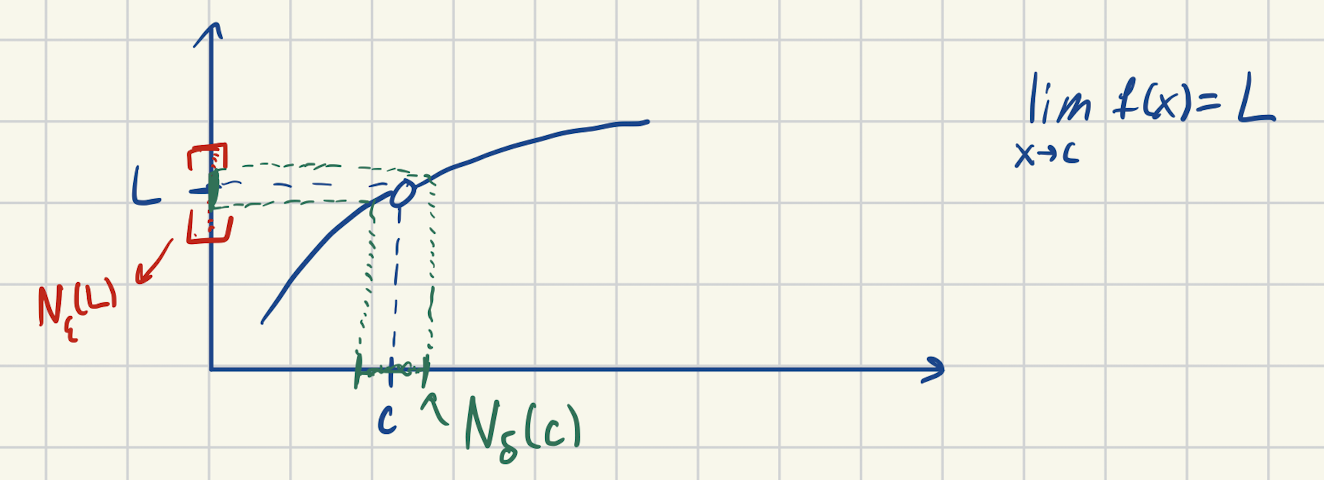
\includegraphics[width=.50\linewidth, center]{/Users/josiahvillarante/GradSchool/Grad-School-Notes/Math230A/Lecture/CH4/images/limit.png}
\end{figure}

\begin{example}
    Let $\begin{cases*}
        f: \R \to \R \\ f(x) = 2x + 5
    \end{cases*}$. Prove that $\lim_{x \to 3}f(x) = 11.$
\end{example}
\begin{proof}
    We want to show $\forall \epsilon > 0 ~\exists \delta > 0 \st \text{if $0 < |x-3| < \delta$, then $|f(x) - 11| < \epsilon$.}$ Let $\epsilon > 0$ be given. Our goal is to find $\delta > 0 \st$
    \begin{equation*}
        \text{if $0 < |x-3| < \delta$ then $|f(x) - L| < \epsilon$.} \tag{$*$}
    \end{equation*}
    \begin{info}
        \begin{align*}
            |f(x) - 11| <\epsilon &\iff |2x+5 - 11| < \epsilon \\ &\iff |2x-6| <\epsilon \\ &\iff 2|x-3| < \epsilon \\ &\iff |x-3| < \frac{\epsilon}{2}.
        \end{align*}
        So, in order to ensure that $(*)$ holds, we need to find $\delta > 0$ such that
        $$\text{if $0 < |x-3| < \delta$, then $|x-3| < \frac{\epsilon}{2}.$}$$ 
    \end{info}
    Let $\delta = \frac{\epsilon}{2}$. For any $x$ with $0 < |x-3| < \delta$, we have
    $$|f(x) - L| = |2x+5 -11| = 2|x-3| < 2 \cdot \delta = 2 \cdot \frac{\epsilon}{2} = \epsilon.$$\qed
\end{proof}

\begin{example}
    Let $\begin{cases*}
        f: \R \to \R \\ f(x) = x^2
    \end{cases*}.$ Prove that $\lim_{x \to 2}f(x) = 4.$
\end{example}
\begin{proof}
    We want to show $\forall \epsilon > 0 ~\exists \delta > 0 \st \text{if $0 < |x-2| < \delta$ then $|f(x) -4| < \epsilon$.}$ Let $\epsilon > 0$ be given. Our goal is to find a number $\delta > 0$ such that
    \begin{equation*}
        \text{if $0 < |x-2| < \delta$ then $|f(x) - 4| < \epsilon$} \tag{$*$}
    \end{equation*}
    \begin{info}
        $$|f(x) - 4| \iff |x^2 -4| < \epsilon \iff |x-2| \cdot |x+2| < \epsilon.$$
        It would be great if we could bound $|x+2|$ with an expression that is easier to work with. Note that for $0 < \delta < 1$ and $0 < |x-2| < \delta$ we have 
        $$|x+2| = |(x-2) + 4| \leq |x-2| + 4 < \delta + 4 \leq 5.$$
        Thus, in order to ensure $(*)$ holds, it is enough to find $0 < \delta \leq 1$ \st
        $$\text{if $0 < |x+2| < \delta$ then $5|x-2| < \epsilon.$}$$
    \end{info}
    Let $\delta = \min \{1, \frac{\epsilon}{5}\}.$ For any $x$ with $0<|x-2|<\delta$ we have 
    $$|f(x) - 4| = |x^2 - 4| = |x-2| \cdot |x+2| < 5 |x-2| \leq 5\left(\frac{\epsilon}{5}\right) = \epsilon.$$
\end{proof}

\begin{example}
    Let $\begin{cases*}
        f: \R \to (\R, \overset{\sim}{d}) \\ f(x) = x^2
    \end{cases*}$ where $\overset{\sim}{d}$ is the discrete metric. Prove that $\lim_{x \to 2}f(x)$ does not exist.
\end{example}
\begin{proof}
    For the sake of contradiction, suppose $\lim_{x \to 2}f(x) = L.$ Then,
    $$\forall \epsilon > 0 ~\exists \delta > 0 \st \text{if $0<|x-2|<\delta$ then $\overset{\sim}{d}(f(x),L)<\epsilon.$}$$
    In particular, for $\epsilon = \frac{1}{2}$,
    $$\exists delta > 0 \st \text{if $0 < |x-2| < \delta$ then $\overset{\sim}{d}(f(x), L) , \frac{1}{2}$.}$$
    Note that
    $$\overset{\sim}{d}(f(x), L) < \frac{1}{2} \implies \overset{\sim}{d}(f(x), L) = 0 \implies f(x) = L.$$
    So,
    $$\exists \delta\ > 0 \st \text{if $2-\delta < x < 2 + \delta, ~x \not = 2,$ then $x^2 = L.$}$$
    Obviously, it is not the case that for all $x\in (2-\delta, 2+\delta), ~x^2$ is equal to a fixed number $L$. Therefore $\lim_{x\to 2}f(x)$ does not exist. \qed
\end{proof}

\begin{theorem}[Sequential Criterion for Limits of Functions] \leavevmode \\
    \label{thm4.2}
    Let $(X,d)$ and $(Y, \overset{\sim}{d})$ be metric spaces, let $E\subseteq X$ be nonempty, and leet $f: X \to Y$. The following are equivalent:
    \begin{enumerate}[$(i)$]
        \item $\lim \limits_{x\to c} f(x) = L$
        \item For all sequences $(a_n)$ in $E \backslash \{c\}$ satisfying $a_n \to c$, we have $f(a_n) \to L$
    \end{enumerate}
\end{theorem}

\begin{proof}
    \begin{description}
        \item[$(i) \implies (ii)$:] \leavevmode \\
        Let $\lim \limits_{x \to c} f(x) = L.$ We want to show that for all $(a_n)$ in $E \backslash \{c\}$ satisfying $a_n \to c$, we have $f(a_n) \to L$. Let $(a_n)$ be a sequence in $E \backslash \{c\}$ such that $a_n \to c$. Our goal is to show that $f(a_n) \to L.$ That is, we want to show
        $$\forall \epsilon > 0 ~\exists N \st \forall n > N ~~\overset{\sim}{d}(f(a_n), L) < \epsilon.$$
        Let $\epsilon > 0$ be given. Our goal is to find $N$ such that
        \begin{equation*}
            \text{if $n > N$ then $\overset{\sim}{d}(f(a_n), L) < \epsilon$} \tag{$*$}
        \end{equation*}
        We have
        \begin{enumerate}[$(I)$]
            \item $\lim \limits_{x \to c} = L \implies \exists \delta > 0 \st \forall x \in \nbhds{\delta}{X}{c} \cap (E \backslash \{c\}) ~~f(x) \in \nbhds{\epsilon}{Y}{L}$
            \item $\lim a_n = c \implies \exists \hat{N} \st \forall n > \hat{N} ~~a_n \in \nbhds{\delta}{X}{c}$
        \end{enumerate}
        We claim that this $\hat{N}$ can be used as the $N$ that we were looking for. Indeed, if we let $N = \hat{N}$, then $(*)$ holds: \\
        For $n > N,$ we have:
        \begin{align*}
            (II) \implies
            \begin{rcases*}
                a_n \in \nbhds{\delta}{X}{c} \\
                a_n \in E \backslash \{c\}
            \end{rcases*}
            &\implies a_n \in \nbhds{\delta}{X}{c} \cap (E \backslash \{c\}) \\
            &\overset{(I)}{\implies} f(a_n) \in \nbhds{\epsilon}{Y}{L}.
        \end{align*} 

        \item[$(ii) \implies (i)$:] \leavevmode \\
        Suppose for all $(a_n) \in E \backslash \{c\}$ satisfying $a_n \to c$, we have $f(a_n) \to L.$ We want to show $\lim \limits_{x \to c} f(x) = L.$ For the sake of contradiction, suppose $\lim \limits_{x \to c} f(x) \not = L$. That is, assume
        $$\sim \left(\forall \epsilon > 0 ~\exists \delta > 0 \st \forall x \in \nbhds{\delta}{X}{c}\cap (E \backslash \{c\}) ~~f(x) \in \nbhds{\epsilon}{Y}{L}\right).$$
        That is,
        $$\exists \epsilon > 0 \st \forall \delta > 0 ~\exists x \in \nbhds{\delta}{X}{c} \cap (E \backslash \{c\}) \st f(x) \not \in \nbhds{\epsilon}{Y}{L}.$$
        So,
        \begin{align*}
            &\delta = 1 &&\exists x_1 \in E\backslash\{c\} \text{ satisfying $d(x_1, c) < 1$ but for which $\overset{\sim}{d}(f(x), L) \geq \epsilon$} \\
            &\delta = \frac{1}{2} &&\exists x_2 \in E\backslash\{c\} \text{ satisfying $d(x_2, c) < \frac{1}{2}$ but for which $\overset{\sim}{d}(f(x), L) \geq \epsilon$} \\
            &\delta = \frac{1}{3} &&\exists x_3 \in E\backslash\{c\} \text{ satisfying $d(x_3, c) < \frac{1}{3}$ but for which $\overset{\sim}{d}(f(x), L) \geq \epsilon$} \\
            \vdots \\
            &\delta = \frac{1}{n} &&\exists x_n \in E\backslash\{c\} \text{ satisfying $d(x_n, c) < \frac{1}{n}$ but for which $\overset{\sim}{d}(f(x), L) \geq \epsilon$}
        \end{align*}
        In this way, we obtain a sequence $(x_n)$ in $E\backslash \{c\} \st x_n \to c$, but for which $\overset{\sim}{d}(f(x_n), L) \geq \epsilon,$ and so $f(x_n) \not \to L.$ This contradicts our assumption.
    \end{description}
    \qed
\end{proof}

\begin{example} \leavevmode \\
    Let $f: \R \backslash \{0\} \to \R$ be defined by $f(x) = \sin\frac{1}{x}.$ Prove that $\lim \limits_{x \to 0} f(x)$ does not exist.
\end{example}

\begin{proof}
    Let $a_n = \frac{1}{2n \pi}, ~b_n = \frac{1}{2n \pi + \pi / 2}.$ Clearly, $(a_n)$ and $(b_n)$ are sequences in $\R \backslash \{0\}$ and $\lim \limits_{n \to \infty} a_n = 0 = \lim \limits_{n \to \infty} b_n.$ However,
    \begin{align*}
        &\lim \limits_{n \to \infty} f(a_n) = \lim \limits_{n \to \infty} \sin \frac{1}{a_n} = \lim \limits_{n \to \infty} \sin (2n\pi) = \lim \limits_{n \to \infty} 0 = 0 \\
        &\lim \limits_{n \to \infty} f(b_n) = \lim \limits_{n \to \infty} \sin \frac{1}{b_n} = \lim \limits_{n \to \infty} \sin (2n\pi + \pi / 2) = \lim \limits_{n \to \infty} 1 = 1 
    \end{align*}
    So, $\lim f(a_n) \not = \lim f(b_n)$. Therefore, $\lim \limits_{x \to 0}\sin \frac{1}{x}$ does not exist.
\end{proof}

\begin{theorem} [Algebraic Limit Theorem for Functions] \leavevmode \\
    \label{thm4.4}
    Let $(x,d)$ be a metric space, $E\subseteq X$ be nonempty, $c \in E'$, and $f,g:E \to \R.$ Assume
    $$\lim \limits_{x \to c} f(x) = L \text{ and } \lim \limits_{x \to c} g(x) = M.$$
    Then
    \begin{enumerate}[$(i)$]
        \item For all $k \in \R ~~\lim \limits_{x \to c}\left(k f(x)\right) = kL$
        \item $\lim \limits_{x \to c} \left(f(x) + g(x)\right) = L+M$
        \item $\lim \limits_{x \to c} \left(f(x) \cdot g(x)\right) = L \cdot M$
        \item $\lim \limits_{x \to c} f(x)/g(x) = L / M,$ provided $M \not = 0$
    \end{enumerate}
\end{theorem}

\begin{proof}
    All of these items follow immediately from the Algebraic Limit Theorem for sequences and the Sequential Criterion for Limits of Functions. \qed
\end{proof}
\newpage

\section{Continuity of a Function}
\begin{definition}[Calculus Definition for Continuity] \leavevmode \\
    Let $(X,d)$ and $(Y, \overset{\sim}{d})$ be metric spaces. Let $E \subseteq X, ~c \in E',$ and $f: E \to Y$. We say $f$ is continuous at $c$ if all the following three conditions hold:
    \begin{enumerate}[$(i)$]
        \item $c \in E ~(\text{$f$ is defined at $c$})$
        \item $\lim \limits_{x \to c}f(x)$ exists
        \item $\lim \limits_{x \to c}f(x) = f(c)$
    \end{enumerate}
\end{definition}

\begin{remark}
    Let $f: E\subseteq (X, d) \to (Y, \overset{\sim}{d})$, and let $c \in E \cap E'.$ Then the following statements are equivalent:
    \begin{enumerate}[$(i)$]
        \item $\lim \limits_{x\to c}f(x) = f(c)$
        \item $\forall \epsilon > 0 ~\exists \delta > 0 \st \text{if $d(x,c) < \delta ~(x \in E),$ then $\overset{\sim}{d}(f(x), f(c)) < \epsilon$}$
        \item $\forall \epsilon > 0 ~\exists \delta > 0 \st \text{if $\forall x \in \nbhds{\delta}{X}{c}\cap E,$ then $f(x) \in \nbhds{\epsilon}{Y}{f(c)}$}$
        \item For every $\epsilon$-neighborhood $\nbhds{\epsilon}{Y}{f(c)}$ of $f(c)$, there exists a $\delta$-neighborhood $\nbhds{\delta}{X}{c}$ of $c \st$the image of $\nbhds{\delta}{X}{c}\cap E$ is contained in $\nbhds{\epsilon}{Y}{f(c)}.$
    \end{enumerate}
\end{remark}

\begin{definition}[General Definition of Continuity] \leavevmode \\
    Let $(x,d)$ and $(Y, \overset{\sim}{d})$ be two metric spaces, and let $E$ be a nonempty set in $X$. Let $c \in E$ and $f: E \to Y$. We say $f$ is continuous at $c$ if any of the following equivalent statements hold:
    \begin{enumerate}[$(i)$]
        \item $\forall \epsilon > 0 ~\exists \delta > 0 \st \text{ if $d(x,c) < \delta,$ then $\overset{\sim}{d}(f(x), f(c)) < \epsilon$}$
        \item $\forall \epsilon > 0 ~\exists \delta > 0 \st \forall x \in \nbhds{\delta}{X}{c}\cap E ~~f(x)\in \nbhds{\epsilon}{Y}{f(c)}$
        \item For every $\epsilon$-neighborhood $\nbhds{\epsilon}{Y}{f(c)}$ of $f(c)$, there exists a $\delta$-neighborhood $\nbhds{\delta}{X}{c}$ of $c$ such that the image of $\nbhds{\delta}{X}{c}\cap E$ is contained in $\nbhds{\epsilon}{Y}{f(c)}$.
    \end{enumerate}
\end{definition}
\begin{figure}[h]
    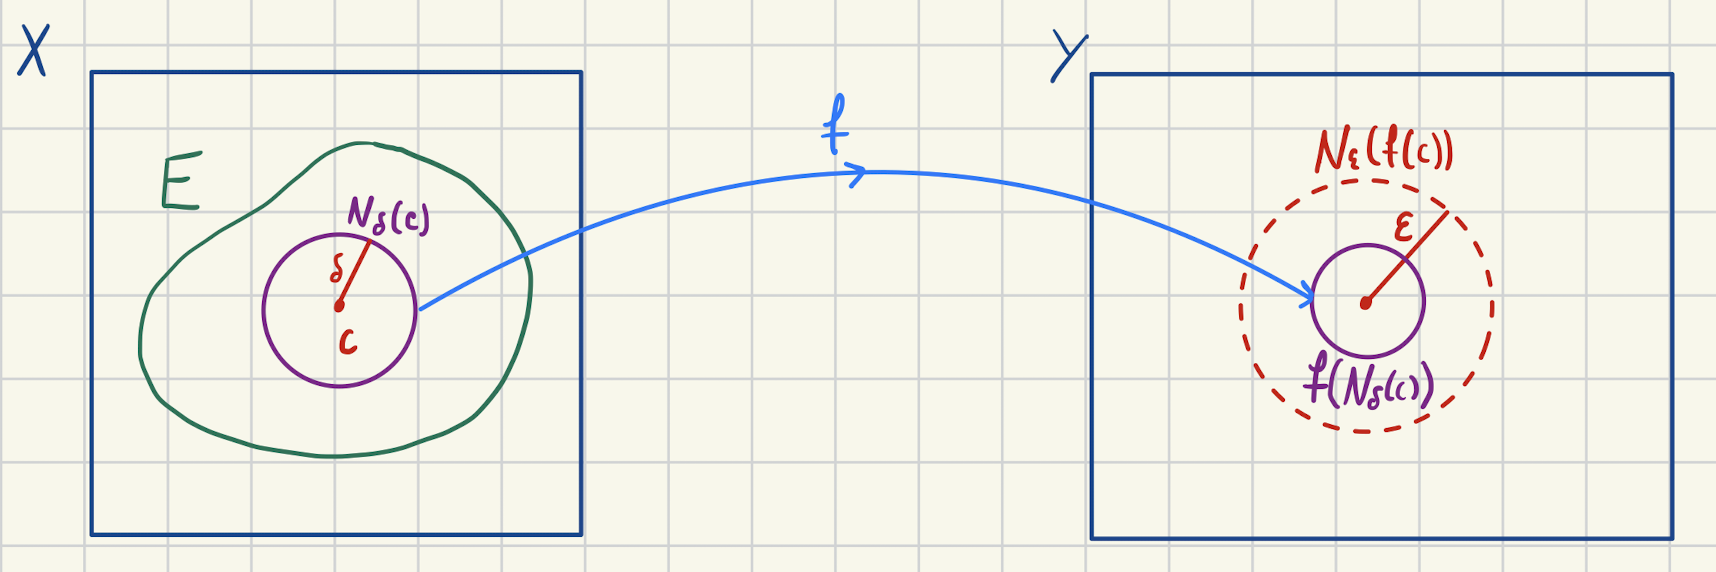
\includegraphics[width=.75\linewidth, center]{/Users/josiahvillarante/GradSchool/Grad-School-Notes/Math230A/Lecture/CH4/images/continuous at c.png}
\end{figure}

\begin{definition}[Continuous Function] \leavevmode \\
    Let $f:E\subseteq X \to Y$. We say $f$ is continuous if it is continuous at every point of $E$.
\end{definition}

\begin{theorem}[Characterization of Continuity via Sequences] \leavevmode \\
    Let $f: E\subseteq X \to Y$. Let $c \in E.$ The following two statements are equivalent:
    \begin{enumerate}[$(i)$]
        \item $f$ is continuous at $c$
        \item For all sequences $(a_n)$ in $E$ satisfying $a_n \to c$ we have $f(a_n) \to f(c)$ 
    \end{enumerate}
\end{theorem}

\begin{proof}
    \begin{description}
        \item[$(i) \implies (ii)$:] \leavevmode \\
        Suppose $f$ is continuous at $c$. Let $(a_n)$ be a sequence in $E$ such that $a_n \to c.$ Our goal is to show that $f(a_n) \to f(c)$, that is, we want to show
        $$\forall \epsilon > 0 ~\exists N \st \forall n > N ~~\overset{\sim}{d}(f(a_n), f(c)) < \epsilon.$$
        Let $\epsilon > 0$ be given. Our goal is to find $N$ such that
        \begin{equation*}
            \text{if $n > N$, then $\overset{\sim}{d}(f(a_n), f(c)) < \epsilon$} \tag{$*$}
        \end{equation*}
        We have
        \begin{enumerate}[$(I)$]
            \item $f$ is continuous at $c \implies \exists \delta > 0 \st \forall x \in \nbhds{\delta}{X}{c}\cap E ~~f(x) \in \nbhds{\epsilon}{Y}{f(c)}$
            \item $a_n \to c \implies \exists \hat{N} \st \forall n > \hat{N} ~~a_n \in \nbhds{\delta}{X}{c}$
        \end{enumerate}
        We claim that we can use $\hat{N}$ as the $N$ that we were looking for. Indeed, if $n > \hat{N}$, then
        \begin{align*}
            (II) \implies
            \begin{rcases*}
                a_n \in \nbhds{\delta}{X}{c} \\
                a_n \in E
            \end{rcases*}
            &\implies a_n \in \nbhds{\delta}{X}{c}\cap E \\
            &\overset{(I)}{\implies} f(a_n) \in \nbhds{\epsilon}{Y}{f(c)}.
        \end{align*}

        \item[$(ii) \implies (i)$:] \leavevmode \\
        Suppose every sequence $(a_n)$ in $E$ such that $a_n \to c$, we have $f(a_n) \to f(c)$. We want to show $f$ is continuous at $c$.
        \begin{info}
            $f$ is continuous at $c \iff \forall \epsilon > 0 ~\exists \delta > 0 \st $ if $x \in \nbhds{\delta}{X}{c}\cap E$ then $f(x) \in \nbhds{\epsilon}{Y}{f(c)}$ \\
            As we discussed last time:
            \begin{enumerate}[$*)$]
                \item if $c \in E \backslash E'$, $f$ is continuous at $c$
                \item if $c \in E'$, then $f$ is continuous at $c \iff \lim \limits_{x \to c}f(x) = f(c)$
            \end{enumerate}
        \end{info}
        We may consider two cases:
        \begin{description}
            \item[Case 1: $c \in E \backslash E'$] ($c$ is an isolated point of $E$) \leavevmode \\
            Any function is continuous at any isolated point of its domain.
            \item[Case 2: $c\in E'$] \leavevmode \\
            It is enough to show that $\lim \limits_{x \to c} f(x) = f(c)$. By the sequential criterion for limits of functions, it is enough to show that
            $$\text{if $(a_n)$ is a sequence in $E \backslash \{c\} \st a_n \to c$, then $f(a_n) \to f(c)$}$$
            But this is a direct consequence of the assumption that
            $$\text{if $(a_n)$ is a sequence in $E \st a_n \to c$, then $f(a_n) \to f(c)$}$$
        \end{description}
    \end{description}
    \qed
\end{proof}

\begin{corollary}[Criterion for Discontinuity]\leavevmode \\
    If you can find one sequence $(a_n)$ in $E$ such that $a_n \to c$, but $f(a_n) \not \to f(c)$, that shows $f$ is not continuous at $c$.
\end{corollary}

\begin{example}
    Prove that the Dirichlet function
    $$f: \R \to \R ~~f(x) = \begin{cases*}
        1 \text{ if } x \in \Q \\
        0 \text{ if } x \not \in \Q
    \end{cases*}$$
    is discontinuous everywhere.
\end{example}

\begin{proof}
    Let $c\in \R$. We will show that $f$ is discontinuous at $c$.
    \begin{description}
        \item[Case 1: $c \in \R \backslash \Q$] ($f(c) = 0$) \leavevmode \\
        Let $(q_n)$ be a sequence of rational numbers such that $q_n \to c.$ Note that
        $$\forall n ~q_n \in \Q \implies \forall n ~f(q_n) = 1 \implies \lim \limits_{n \to \infty}f(q_n) = \lim \limits_{n\to \infty}1 = 1.$$ 
        Therefore,
        $$
        \begin{rcases*}
            q_n \to c \\
            f(q_n) \not \to f(c) = 0
        \end{rcases*} \implies f \text{ is not continuous at $c$}.
        $$
        \item[Case 2: $c \in \Q$] ($f(c) = 1$)\leavevmode \\
        Let $(r_n)$ be a sequence of irrational numbers such that $r_n \to c.$ Note that
        $$\forall n ~r_n \in \R \backslash \Q \implies \forall n ~f(r_n) = 0 \implies \lim \limits_{n\to \infty}f(r_n) = \lim \limits_{n \to \infty}0 = 0.$$
        Therefore,
        $$
        \begin{rcases*}
            r_n \to c \\
            f(r_n) \not \to f(c) = 1
        \end{rcases*} \implies f \text{ is not continuous at $c$}.
        $$
        \qed
    \end{description}
\end{proof}

\begin{example}
    Prove that $f: (\R, d) \to \R$ (where $d$ is the discrete metric) defined by
    $$
    f(x) = \begin{cases*}
        1 &\text{ if $x\in \Q$} \\
        0 &\text{ if $x \not \in \Q$}
    \end{cases*}
    $$
    is continuous everywhere.
\end{example}

\begin{proof}
    Let $c\in \R.$ Our goal is to show that $f$ is coninuous at $c.$ That is, we want to show
    $$\forall \epsilon > 0 ~\exists \delta > 0 \st \text{if $d(x,c) < \delta$, then $|f(x) - f(c)| < \epsilon.$}$$
    Let $\epsilon > 0$ be given. Our goal is to find $\delta > 0$ such that 
    \begin{equation*}
        \text{if $d(x,c) < \delta$, then $|f(x) - f(c)| < \epsilon$}
        \tag{$*$}
    \end{equation*}
    Regardless of the expression of $f$, $(*)$ holds with $\delta = \frac{1}{2}$. Indeed, if $d(x,c) < \frac{1}{2}$, then $d(x,c) = 0,$ so $x=c$ and therefore $|f(x) - f(c)| = 0 < \epsilon,$ as desired. \qed
\end{proof}

\begin{example}
    Let $(X, \|\cdot\|)$ be a normed space. Prove that $\|\cdot\|: X \to \R$ is continuous.
\end{example}

\begin{proof}
    Let $c\in X$. We will prove that $\|\cdot\|$ is continuous at $c.$ That is, we will show
    \begin{equation*}
        \forall \epsilon > 0 ~\exists \delta > 0 \st \text{if $\|x-c\| < \delta$, then $\left|\|x\| - \|c\|\right| < \epsilon$.}
        \tag{$*$}
    \end{equation*}
    It follows immediately from the inequality
    $$\left|\|x\|-\|c\|\right|\leq \|x-c\|$$
    that $(*)$ holds with $\delta = \epsilon.$ \qed
\end{proof}

\begin{corollary}
    If $x_n \to x$ in $X$, then $\|x_n\| \to \|x\|$ in $\R$.
\end{corollary}

\begin{example}
    Let $(X,d)$ be a metric space. Let $p\in X.$ Define $f: X \to \R$ by $f(x) = d(p,x)$. Prove that $f$ is continuous.
\end{example}

\begin{proof}
    Let $c\in X$. our goal is to show that 
    $$\forall \epsilon > 0 ~\exists \delta > 0 \st \text{if $d(x,c) < \delta$, then $|d(p,x) - d(p, c)| < \epsilon.$}$$
    Let $\epsilon > 0$ be given. Our goal is to find $\delta > 0$ such that
    \begin{equation*}
        \text{if $d(x,c) < \delta,$ then $|d(p,x) - d(p,c)| < \epsilon$}
        \tag{$*$}
    \end{equation*}
    It follows immediately from the inequality
    $$|d(p,x) - d(p,c)| \leq d(x,c)$$
    that $(*)$ holds with $\delta = \epsilon.$ \qed
\end{proof}

\begin{example}
    Consider $C[0,1] = \{f:[0,1]\to \R: \text{$f$ is continuous}\}$ equipped with the norm
    $$\|f\|_{\infty} = \max \limits_{0\leq x \leq 1} \left|f(x)\right|.$$
    Prove that $\begin{cases*}
        T: C[0,1] \to \R \\
        T(f) = f(\frac{1}{2})
    \end{cases*}$ is continuous.
\end{example}

\begin{proof}
    Let $g\in C[0,1].$ Our goal is to show that $T$ is continuous at $g$. To this end, it is enough to show that if $g_n \to g$ in $\left(C[0,1], \|\cdot\|_{\infty}\right)$, then $T(g_n) \to T(g)$ in $\R$. We have 
    \begin{align*}
        g_n \to g \text{ in } \left(C[0,1], \| \cdot \|_{\infty}\right)
        &\implies \|g_n - g\|_{\infty} \to 0 \text{ as } n \to \infty \\
        &\implies \max \limits_{0 \leq x \leq 1} \left|g_n(x) - g(x)\right| \to 0 \text{ as } n \to \infty \\
        0 \leq \left|g_n (1/2) - g(1/2)\right| &\leq \max\left|g_n(x) - g(x)\right| \\
        &\implies \left|g_n(1/2) - g(1/2)\right| \to 0 \text{ as } n \to \infty &&\text{(squeeze theorem)} \\
        &\implies g_n(1/2) \to g(1/2) \text{ in } \R \\
        &\implies T(g_n) \to T(g) \text{ in } \R
    \end{align*}
    \qed
\end{proof}

\begin{theorem}[Algebraic Continuity Theorem] \leavevmode \\
    \label{thm4.9}
    Assume $f:E \subseteq (X,d) \to \R$ and $g:E \subseteq (X,d) \to \R$ are continuous at $c\in E$. Then
    \begin{enumerate}[$(i)$]
        \item $kf(x)$ is continuous at $c$ for all $k\in\R$
        \item $f(x) + g(x)$ is continuous at $c$
        \item $f(x)g(x)$ is continuous at $c$
        \item $f(x)/g(x)$ is continuous at $c$ provided $g(c) \not = 0$
    \end{enumerate}
\end{theorem}

\begin{proof} \leavevmode
    These are direct consequences of the algebraic limit theorem for sequences and the characterization of continuity via sequences. For example, let's prove $(iii)$: \\
    By characterization of continuity via sequences, it is enough to show that if $(a_n)$ is a sequence in $E$ such that $a_n \to c$, then $f(a_n)g(a_n) \to f(c)g(c).$ Let $(a_n)$ be such a sequence. We have
    \begin{equation*}
        \begin{rcases*}
            f \text{ is continuous at } c \\
            a_n \to c
        \end{rcases*} \implies f(a_n) \to f(c)
        \tag{$*$}
    \end{equation*}
    \begin{equation*}
        \begin{rcases*}
            g \text{ is continuous at } c \\
            a_n \to c
        \end{rcases*} \implies g(a_n) \to g(c)
        \tag{$**$}
    \end{equation*}
    In what follows from $(*),(**)$, and the algebraic limit theorem for sequences of real numbers that
    $$f(a_n)g(a_n) \to f(c)g(c)$$
    as desired. \qed
\end{proof}

\begin{theorem}[Composition of Continuous Functions is Continuous] \leavevmode \\
    \label{thm4.7}
    Let $(X,d), (Y,\overset{\sim}{d}),$ and $(Z, \overset{\approx}{d})$ be metric spaces. Let $A$ be a nonempty subset of $X$ and $B$ be a nonempty subset of $Y$. Let $f: A \to Y$ and $g: B \to Z$ such that $f(A) \subseteq B.$ Suppose $f$ is continuous at $c \in A$, and $g$ is continuous at $f(c) \in B$. Then $g \circ f: A \to Z$ is continuous at $c \in A$.
\end{theorem}

\begin{proof}
    It is enough to show that if $(a_n)$ is a sequence in $A$ such that $a_n \to c$, then $(g\circ f)(a_n) \to (g \circ f)(c).$ Let $(a_n)$ be such a sequence. We have 
    \begin{align*}
        \begin{rcases*}
            f \text{ is continuous at } c \\
            a_n \to c
        \end{rcases*} &\implies f(a_n) \to f(c) \\
        \begin{rcases*}
            g \text{ is continuous at } f(c) \\
            f(a_n) \to f(c)
        \end{rcases*} &\implies g(f(a_n)) \to g(f(c)).
    \end{align*}
    So, $(g \circ f)(a_n) \to (g \circ f)(c)$ as desired. \qed
\end{proof}

\begin{example}
    If $f: X \to \R$ and $g: X \to \R$ are continuous, then
    $$\text{$\max\{f,g\}$ and $\min\{f,g\}$}$$
    are also continuous.
\end{example}
\begin{align*}
    \max\{a,b\} &= \frac{a+b}{2} + \frac{|a-b|}{2} \\
    \min\{a,b\} &= \frac{a+b}{2} - \frac{|a-b|}{2}
\end{align*}

\begin{example}\leavevmode \\
    \begin{enumerate}[$(1)$]
        \item If $E$ is a metric subspace of $X$, then $$i: E \to X, i(x) = X$$ is continuous.
        \item If $f:X \to Y$ is continuous and $E\subseteq X,$ then $f|_{E}: E \to X$ is continuous.
        \item If $\begin{cases*}
            f: X \to Y \text{ is continuous} \\
            Y \text{ is a metric space}
        \end{cases*}$, then $i \circ f: X \to Z$ is continuous.
    \end{enumerate}
\end{example}
\newpage

\section{Topological Continuity}
So far, we have learnt two equivalent descriptions of the concept of continuity for functions $f: (X,d) \to (Y, \overset{\sim}{d}):$
(1) $f$ is continuous if and only if
$$\forall c \in X ~\forall \epsilon > 0 ~\exists \delta_{\epsilon, c} > 0 \st \text{if $d(x,c) < \delta_{\epsilon, c}$ then $\overset{\sim}{d}(f(x), f(c)) < \epsilon$}$$
(2) $f$ is continuous if and only if
$$\forall c \in X ~a_n \to c \implies f(a_n) \to f(c).$$
Our next goal is to describe a third (equivalent) description of continuity. \\ \\
In Math 130: $f:\R \to \R, a_n \to c$ in $\R$
$$a_n \to c \iff \forall \epsilon > 0 ~\exists N \st \forall n > N ~~|a_n - c| < \epsilon.$$
Math 230: $(X,d)$
\begin{align*}
    &\text{Level 1:} && a_n \to c \iff \forall \epsilon > 0 ~\exists N \st \forall n > N ~~d(a_n, c) < \epsilon \\
    &\text{Level 2:} && a_n \to c \iff \forall \nbhd{\epsilon}{c} ~\exists N \st \forall n > N ~~a_n \in \nbhd{\epsilon}{c}
\end{align*}

\noindent
Topology: $X$ is a set \\
We tell our audience which subsets of $X$ should be considered open.
$$a_n \to c \iff \forall U_{\text{open}} \text{ containing } c ~\exists N \st \forall n > N ~~a_n \in U$$

\begin{theorem}[Topological Characterization of Continuity] \leavevmode \\
  \label{thm4.8}
  Let $(X,d)$ and $(Y, \overset{\sim}{d})$ be metric spaces, and let $f: X \to Y.$ The following are equivalent:
  \begin{enumerate}[$(i)$]
    \item $f$ is continuous
    \item For every open set $B \subseteq Y, ~ f^{-1}(B)$ is open in $X$.
  \end{enumerate}  
\end{theorem}

\begin{proof}
    $(i) \implies (ii)$: Suppose $f$ is continuous. Let $B$ be an open set in $Y$. Our goal is to show $f^{-1}(B)$ is open in $X$. That is, we want to show every point of $f^{-1}(B)$ is an interior point. Let $p \in f^{-1}(B).$ Our goal is to show there exists $\delta > 0$ such that $\nbhds{\delta}{X}{p} \subseteq f^{-1}(B)$. We have
    $$p \in f^{-1}(B) \implies f(p) \in B \overset{B \text{ is open}}{\implies} \exists \epsilon > 0 \st \nbhds{\epsilon}{Y}{f(p)} \subseteq B.$$
    Since $f$ is continuous at $p$, there exists $\hat{\delta} > 0 \st$
    $$\forall x \in \nbhds{\hat{\delta}}{X}{p} ~~f(x) \in \nbhds{\epsilon}{Y}{f(p)} \subseteq B.$$
    Clearly, $\nbhds{\hat{\delta}}{X}{p} \subseteq f^{-1}(B)$, so we can use this $\hat{\delta}$ as the $\delta$ we were looking for. \\ \\
    $(ii) \implies (i):$ Assume $\forall B_{\text{open}} \subseteq Y, ~f^{-1}(B)$ is open in $X$. Let $c\in X$. We will prove $f$ is continuous at $c$. That is, our goal is to show that 
    $$\forall \epsilon > 0 ~\exists \delta > 0 \st \text{if $\nbhds{\delta}{X}{c}$ then $f(x) \in \nbhds{\epsilon}{Y}{f(c)}$.}$$
    Let $\epsilon > 0$ be given. Our goal is to find $\delta > 0$ such that
    \begin{equation*}
        \nbhds{\delta}{X}{c} \subseteq f^{-1}\left(\nbhds{\epsilon}{Y}{f(c)}\right)
    \end{equation*}
    Since $\nbhds{\epsilon}{Y}{f(c)}$ is open in $Y$, it follows from the assumption that $f^{-1}\left(\nbhds{\epsilon}{Y}{f(c)}\right)$ is open in $X$. We have
    \begin{align*}
        \begin{rcases*}
            f^{-1}\left(\nbhds{\epsilon}{Y}{f(c)}\right) \text{ is open in $X$} \\
            c \in f^{-1}\left(\nbhds{\epsilon}{Y}{f(c)}\right)
        \end{rcases*} &\implies c \text{ is an interior point of } f^{-1}\left(\nbhds{\epsilon}{Y}{f(c)}\right) \\
        &\implies \exists \delta > 0 \st \nbhds{\delta}{X}{c} \subseteq f^{-1}\left(\nbhds{\epsilon}{Y}{f(c)}\right)
    \end{align*}
    \qed
\end{proof}

\begin{remark}
    $f:(X,d) \to (Y, \overset{\sim}{d})$ is continuous $\iff$ for every closed set $B \subseteq Y$, $f^{-1}(B)$ is closed in $X$.
\end{remark}

\begin{theorem}[Continuity Preserves Compactness] \leavevmode \\
    \label{thm4.14}
    Let $(X,d)$ and $(Y, \overset{\sim}{d})$ be metric spaces and let $E\subseteq X$ be compact. Let $f:E\to Y$ be continuous. Then $f(E)$ is compact in $Y$.
\end{theorem}

\begin{proof}
    Let $\ocover{O}$ be an open cover of $f(E)$. Our goal is to show that this open cover has a finite subcover.
    \begin{recall}
    From set theory, we have:
    \begin{enumerate}[$(1)$]
        \item $f \left(\bigcup \limits_{\alpha \in \Lambda}A_{\alpha}\right) = \bigcup \limits_{\alpha \in \Lambda} f(A_{\alpha})$
        \item $f \left(\bigcap \limits_{\alpha \in \Lambda} A_{\alpha}\right) \subseteq \bigcap \limits_{\alpha \in \Lambda}f(A_{\alpha})$
        \item $f^{-1}\left(\bigcup \limits_{\alpha \in \Lambda} A_{\alpha}\right) = \bigcup \limits_{\alpha \in \Lambda} f^{-1}(A_{\alpha})$
        \item $f^{-1}\left(\bigcap \limits_{\alpha \in \Lambda} A_{\alpha}\right) = \bigcap \limits_{\alpha \in \Lambda} f^{-1}(A_{\alpha})$
        \item $A\subseteq f^{-1}(f(A))$
        \item $f(f^{-1}(B)) \subseteq B$
        \item $f^{-1}(B \backslash C) = f^{-1}(B) \backslash f^{-1}(C)$
        \item $f^{-1}(E^c)=\left(f^{-1}(E)\right)^c$
    \end{enumerate}
    \end{recall}
    We have
    $$f(E) \subseteq \bigcup \limits_{\alpha \in \Lambda} O_{\alpha}.$$
    so
    $$f^{-1}(f(E)) \subseteq f\left(\bigcup \limits_{\alpha \in \Lambda} O_{\alpha}\right).$$
    Since $E \subseteq f^{-1}(f(E))$ and $f^{-1}\left(\bigcup \limits_{\alpha \in \Lambda}O_{\alpha}\right) = \bigcup \limits_{\alpha \in \Lambda}f^{-1}(O_{\alpha})$, we can conclude that 
    $$E \subseteq \bigcup \limits_{\alpha \in \Lambda}f^{-1}(O_{\alpha}).$$
    Note that
    $$\begin{rcases*}
        \forall \alpha \in \Lambda ~O_{\alpha} \text{ is open in $Y$} \\
        f: X \to Y \text{ is continuous}
    \end{rcases*} \implies \forall \alpha \in \Lambda ~f^{-1}(O_{\alpha}) \text{ is open in $X$}.$$
    So, $\ocover{f^{-1}(O_{\alpha})}$ is an open cover for $E$. Since $E$ is compact,
    $$\exists \alpha_1, ..., \alpha_n \in \Lambda \st E \subseteq f^{-1}(O_{\alpha_1}) \cup ... \cup f^{-1}(O_{\alpha_n}).$$
    Consequently,
    \begin{align*}
        f(E) &\subseteq f\left(f^{-1}(O_{\alpha_1})\cup ... \cup f^{-1}(O_{\alpha_n})\right) \\
        &= f(f^{-1}(O_{\alpha_1}))\cup ... \cup f(f^{-1}(O_{\alpha_n})) \\
        &\subseteq O_{\alpha_1} \cup ... \cup O_{\alpha_n}.
    \end{align*}
    So, $\{O_{\alpha_1},...,O_{\alpha_n}\}$ is a finite subcover for $f(E)$. \qed
\end{proof}

\begin{theorem} [Extreme Value Theorem] \leavevmode \\
    \label{thm4.15}
    Let $(X,d)$ be a compact metric space.
    \begin{enumerate} [$(i)$]
        \item If $f:(X,d) \to (Y, \overset{\sim}{d})$ is continuous, then $f(X)$ is a closed and bounded set in $Y$.
        \item If $f:(X,d) \to \R$ is continuous, then $f$ attains a maximum value and a minimum value. More precisely, $M=\sup \limits_{x \in X}f(x)$ and $m=\inf \limits_{x \in X}f(x)$ exists, and there exists points $a\in X$ and $b \in X$ such that $f(a) = M$ and $f(b) = m$.
    \end{enumerate}
\end{theorem}

\begin{proof}
    \begin{enumerate}[$(i)$]
        \item By Theorem \ref{thm4.14}, $f(X)$ is compact in $Y$. As we know, any compact set in any metric space is closed and bounded.
        \item By part $(i)$, $f(X)$ is a closed and bounded subset of $\R$. Since $f(X)$ is a bounded set in $\R$, $M = \sup f(X) = \sup \limits_{x\in X} f(x)$ and $m = \inf f(X) = \inf \limits_{x \in X}f(x)$ exist. By Theorem \ref{thm2.28}, $M\in \overline{f(X)}$ and $m \in \overline{f(X)}$. Since $\overline{f(X)} = f(X),$ we conclude that $M\in f(X)$ and $m\in f(X)$. That is,
        $$\exists a \in X \st M = f(a) \text{ and } \exists b \in X \st m = f(b).$$
    \end{enumerate}
    \qed
\end{proof}

\begin{theorem} [Continuity Preserves Connectedness] \leavevmode \\
    \label{thm4.22}
    Let $(X,d)$ and $(Y, \overset{\sim}{d})$ be metric spaces and let $f:X \to Y$ be continuous. Let $E\subseteq X$ be connected. Then $F(E)$ is conected in $Y$.
\end{theorem}

\begin{proof}
    Assume for contradiction that $f(E)$ is not connected. Thus we can write $f(E)$ as a union of two (nonempty) separated sets $A$ and $B$:
    $$f(E)= A\cup B, ~\overline{A}\cap B = \emptyset=A\cap \overline{B}.$$
    Let $G=E\cap f^{-1}(A)$ and $H=E \cap f^{-1}(B).$ In what follows, we'll show that $G$ and $H$ form a separation of the set $E$, which contradicts the assumption that $E$ is connected. We need to show:

    \begin{align*}
        &(1) ~~G, H \not = \emptyset &&(3) ~~\overline{G}\cap H = \emptyset \\
        &(2) ~~G\cup H = E &&(4) ~~G \cap \overline{H} = \emptyset
    \end{align*}

    \begin{enumerate}[$(1)$]
        \item $G$ and $H$ are nonempty: Here, I will show $G \not = \emptyset$ (analogously, we can prove $H$ is nonempty). To this end, we will prove $$f(G) = A ~~~~~\left(f(H) = B \right).$$ We have
        \begin{enumerate}[$(i)$]
            \item $f(G)=f(E\cap f^{-1}(A)) \subseteq f(E) \cap f(f{-1}(A)) \subseteq f(E) \cap A = A$
            \item Let $y\in A$. Then $y\in f(E) \implies \exists x \in E \st f(x) = y.$
            \begin{align*}
                f(x) = y \in A &\implies x \in f^{-1}(A) \\
                &\implies x \in E \cap f^{-1}(A) \\
                &\implies f(x) \in f(E\cap f^{-1}(A)) = f(G) \\
                &\implies y \in f(G) \\
                &\implies A \subseteq f(G).
            \end{align*}
        \end{enumerate}
        
        Thus $f(G) = A$ (and $f(H) = B$), so $G$ is nonempty.

        \item $E = G \cup H$:
        \begin{align*}
            G\cup H &= (E \cap f^{-1}(A)) \cup (E \cap f^{-1}(B)) \\
            &= E \cap [f^{-1}(A) \cup f^{-1}(B)] \\
            &= E \cap [f^{-1}(A \cup B)] \\
            &= E \cap [f^{-1}(f(E))] \\
            &= E &&\left(\text{since } E \subseteq f^{-1}(f(E))\right)
        \end{align*}

        \item $\overline{G} \cap H = \emptyset$ (analogously, $G\cap \overline{H}=\emptyset):$ To this end, it is enough to show that $f(\overline{G})\cap f(H) = \emptyset.$ Note that $f(H) = B$. So, we want to show $f(\overline{G})\cap B = \emptyset$. Since $\overline{A}\cap B$ is empty, it is enough to show that $f(\overline{G}) \subseteq \overline{A}$. We have
        $$G = E \cap f^{-1}(A) \subseteq f^{-1}(A) \subseteq f^{-1}(\overline{A}).$$
        Also,
        $$\begin{rcases*}
            f \text{ is continuous} \\
            \overline{A} \text{ is closed}
        \end{rcases*} \implies f^{-1}(\overline{A}) \text{ is closed in $X$.}$$
        Thus we can write
        $$G \subseteq f^{-1}(A) \implies \overline{G} \subseteq \overline{f^{-1}(\overline{A})} = f^{-1}(A).$$
        Therefore,
        $$f(\overline{G}) \subseteq f(f^{-1}(\overline{A})) \subseteq \overline{A}.$$
    \end{enumerate}
    \qed
\end{proof}

\begin{theorem}[The Intermediate Value Theorem] \leavevmode \\
    \label{thm4.23}
    Let $f:[a,b] \to \R$ be continuous and suppose $f(a) \not = f(b)$. Let $L \in R \st f(a) < L < f(b)$ or $f(b) < L < f(a)$. Then there exists $c \in (a,b) \st f(c) = L.$
\end{theorem}

\begin{proof}
\begin{align*}
    \begin{rcases*}
        f:[a,b] \to \R \text{ is connected} \\
    \end{rcases*}
    &\implies f\left([a,b]\right) \text{ is connected in } \R \\
    &\implies f\left([a,b]\right) \text{ is either a singleton or an interval $I$ in $\R$} \\
    &\implies f\left([a,b]\right) \text{ is an interval $I$ in $\R$} &&(\text{since } f(a) \not = f(b))\\
    &\implies L \in f\left([a,b]\right) &&(\text{since }f(a), f(b) \in I)\\
    &\implies \exists c \in [a,b] \st f(c) = L \\
    &\implies \exists c \in (a,b) \st f(c) = L &&(\text{since }f(a), f(b) \not = L)
\end{align*}
\qed
\end{proof}

\begin{note}
    If $f: X \to Y$ is continuous and bijective, it's not necessarily true that $f^{-1}: Y \to X$ is continuous. For example, $f: (-1,0]\cup [1,2] \to [0,4]$ given by $f(x) = x^2$ is a continuous bijection. However, $f^{-1}: [0,4] \to (-1, 0]\cup [1,2]$ is not continuous: $[0,4]$ is connected, but $f^{-1}\left([0,4]\right)=(-1,0]\cup[1,2]$ is not connected; $[0,4]$ is compact, but $(-1,0]\cup[-1,2]$ is not compact.
\end{note}

\begin{figure}[h]
    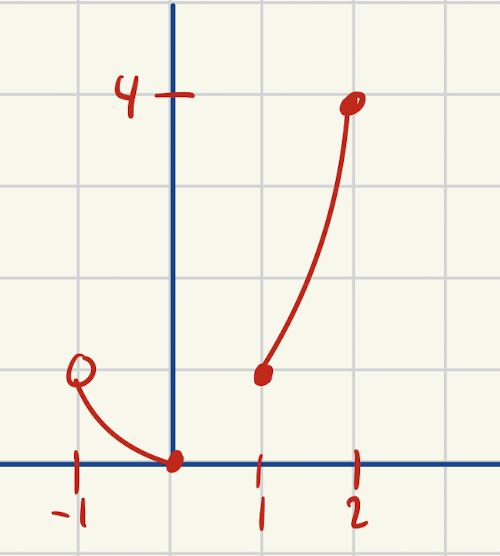
\includegraphics[width=.25\linewidth, center]{/Users/josiahvillarante/GradSchool/Grad-School-Notes/Math230A/Lecture/CH4/images/noncontinuous inverse.png}
\end{figure}

\begin{theorem} \leavevmode \\
    \label{thm4.17}
    Let $(X,d), (Y, \overset{\sim}{d})$ be metric spaces, and suppose $X$ is compact. Let $f:X \to Y$ be continuous and bijective. Then $f^{-1}:Y \to X$ is continuous.
\end{theorem}

\begin{proof}
    It is enough to show tha for every open set $B \subseteq X, (f^{-1})^{-1}(B)$ is open in $Y$. That is, suppose $B$ is open in $X$ and show $f(B)$ is open in $Y$.
    \begin{align*}
        \text{$B$ is open in $X$} &\implies \text{$B^c$ is closed in $X$} \\
        &\implies \text{$B^c$ is compact in $X$} \\
        &\implies \text{$f(B^c)$ is compact in $Y$} \\
        &\implies \text{$f(B^c)$ is closed in $Y$} \\
        &\implies \text{$[f(B^c)]^c$ is open in $Y$} \\
        &\implies \text{$f(B)$ is open in $Y$}
    \end{align*}
    \qed
\end{proof}
\newpage

\section{Uniform Continuity}
Uniform continuity will allow us to extend the domain of our function to the entire metric space.

\begin{theorem}[A Special Case of the Tietze Extension Theorem] \leavevmode \\
    Let $(X,d)$ be a metric space and let $A$ be a nonempty closed set in $X$. If $f:A\to \R$ is continuous, then $f$ has a continuous extension to all of $X$.
\end{theorem}

\begin{theorem} \leavevmode \\
    Let $(X,d)$ be a metric space and let $A$ be a nonempty set in $X$. If $f:A\to \R$ is uniformly continuous on $A$, then $f$ can be extended to a continuous function $\overline{f} : \overline{A} \to \R$.
\end{theorem}

\begin{definition} [Uniformly Continuous] \leavevmode \\
    Let $f: A \subseteq (X,d) \to (Y, \overset{\sim}{d})$ be a function. $f$ is said to be uniformly continuous on $A$ if 
    $$\forall \epsilon > 0 ~\exists \delta_\epsilon \st \forall x, c \in A \text{ if $d(x,c) < \delta_\epsilon$ then $\overset{\sim}{d}(f(x), f(c)) < \epsilon.$}$$
\end{definition}

\begin{note}
    What does it mean to say $f$ is not uniformly continuous on $A$?
    $$\exists \epsilon > 0 \st \forall \delta > 0 ~\exists x,c \in A \text{ satisfying $d(x,c) < \delta$ but $\overset{\sim}{d}(f(x),f(c)) \geq \epsilon$}$$
\end{note}

\begin{example}
    Prove that $f: \R \to \R$ defined by $f(x) = 2x+1$ is uniformly continuous on $\R$.
\end{example}

\begin{proof}
    Our goal is to show that 
    $$\forall \epsilon > 0 ~\exists \delta > 0 \st \forall x,c \in \R \text{ if $|x-c| < \delta$ then $|f(x) - f(c)| < \epsilon$.}$$
    Let $\epsilon > 0$ be given. Our goal is to find $\delta > 0$ such that 
    $$\forall x,c \in \R \text{ if $|x-c| < \delta$ then $|(2x+1) - (2c+1)| < \epsilon.$}$$
    Clearly, we can take $\delta = \epsilon / 2$ (or any positive number less than $\epsilon / 2$). \qed
\end{proof}

\begin{remark}
    It is a direct consequence of our definition of uniform continuity that if $f$ is uniformly continuous on a set $A$ and $\emptyset \not = B \subseteq A$, then $f$ is uniformly continuous on $B$.
\end{remark}

\begin{theorem} \leavevmode \\
    Let $f:A \subseteq (X,d) \to (Y, \overset{\sim}{d})$. If we can find a number $\epsilon_0 > 0$ and two sequences $(x_n)$ and $(c_n)$ in $A$ such that 
    \begin{equation*}
        d(x_n, c_n) \to 0 \text{ and } \forall n ~~\overset{\sim}{d}(f(x_n), f(c_n)) \geq \epsilon_0
        \tag{$*$}
    \end{equation*}
    then $f$ is not uniformly continuous on $A$.
\end{theorem}

\begin{proof}
    Recall that $f$ is not uniformly continuous if and only if 
    $$\exists \epsilon > 0 \st \forall \delta > 0 ~\exists x, c \in A \text{ satisfying $d(x,c) < \delta$ but $\overset{\sim}{d}(f(x), f(c)) \geq \epsilon$.}$$
If $(*)$ holds, then the above statement will hold with $\epsilon = \epsilon_0$. Indeed, given $\delta > 0$, $~~\exists N \st d(x_N, c_N) < \delta$ but $\overset{\sim}{d}(f(x_N), f(c_N)) \geq \epsilon.$ \qed
\end{proof}

\begin{example}
    Prove that $f(x) = x^2$ is not uniformly continuous on $\R$.
\end{example}

\begin{proof}
    Let $x_n = n, ~c_n = n + 1/n.$ We have 
    $$\lim \limits_{n\to \infty} |x_n - c_n| = \lim \limits_{n \to \infty}|-1/n| = 0.$$
    Also, for all $n$,
    \begin{align*}
        |f(x_n) - f(c_n)| &= |n^2 - (n + 1/n)^2| \\
        &= |n^2 - n^2 - 2 - 1 / n^2| \\
        &= |-(x + 1/n^2)| \\
        &= 2 + 1/n^2 \geq 2.
    \end{align*}
    Thus, $f(x) = x^2$ is not uniformly continuous on $\R$. \qed
\end{proof}

\begin{example}
    Prove that $f(x) = \sin \frac{1}{x}$ is not uniformly continuous on $(0,1)$.
\end{example}

\begin{proof}
    Use $x_n = \frac{1}{2n\pi}$ and $c_n = \frac{1}{2n\pi + pi/2}.$
    $$\begin{rcases*}
        \lim x_n = 0 \\
        \lim c_n = 0
    \end{rcases*}
    \implies \lim (x_n - c_n) = 0 \implies \lim |x_n - c_n| = 0.$$
    But for all $n$
    $$|f(x_n) - f(c_n)| = |\sin (2n\pi) - \sin (2n\pi + \pi / 2)| = |0-1| = 1$$
    so $f$ is not uniformly continuous. \qed
\end{proof}

\begin{theorem} \leavevmode \\
    \label{thm4.19}
    Let $f: A \subseteq (X,d) \to (Y, \overset{\sim}{d})$ be continuous and suppose $A$ is compact. Then $f$ is uniformly continuous.
\end{theorem}

\begin{proof}
    For the sake of contradiction, suppose $f$ is not uniformly continuous. Then 
    $$\exists \epsilon > 0 \st \forall \delta > 0 ~\exists x,c \in A \text{ satisfying $d(x,c) < \delta$ but $\overset{\sim}{d}(f(x), f(c)) \geq \epsilon$.}$$
    In particular,
    \begin{align*}
        &\delta = 1 &&\exists x_1, c_1 \in A \text{ satisfying $d(x_1, c_1) < 1$ but $\overset{\sim}{d}(f(x_1), f(c_1)) \geq \epsilon$} \\
        &\delta = \frac{1}{2} &&\exists x_2, c_2 \in A \text{ satisfying $d(x_2, c_2) < \frac{1}{2}$ but $\overset{\sim}{d}(f(x_2), f(c_2)) \geq \epsilon$} \\
        &\delta = \frac{1}{3} &&\exists x_3, c_3 \in A \text{ satisfying $d(x_3, c_3) < \frac{1}{3}$ but $\overset{\sim}{d}(f(x_3), f(c_3)) \geq \epsilon$} \\
        \vdots
    \end{align*}
    In this way, we will obtain two sequences $(x_n)$ and $(c_n)$ in $A$ such that 
    \begin{enumerate}[$(i)$]
        \item $0 \leq d(x_n, c_n) < \frac{1}{n} ~~\forall n$
        \item $\overset{\sim}{d}(f(x_n), f(c_n)) \geq \epsilon ~~ \forall n$
    \end{enumerate}
    We have
    $$\begin{rcases*}
        A \text{ is compact } \implies A \text{ is sequentially compact} \\
        (x_n) \text{ is a sequence in } A
    \end{rcases*}
    \implies (x_n) \text{ has a subsequence $(x_{n_k})$ that converges to a point in $A$}$$
    Let $x = \lim \limits_{k \to \infty}x_{n_k}.$ Let $(c_{n_k})$ be the corresponding subsequence of $(c_n)$. We have 
    $$0 \leq d(c_{n_k}, x) \leq d(c_{n_k}, x_{n_k}) + d(x_{n_k}, x)$$
    So, $\lim \limits_{k\to \infty} c_{n_k} = x.$ Therefore, $(x_{n_k})$ and $(c_{n_k})$ are two sequences in $A$ that converge to $x\in A$.
    \begin{align*}
        x_{n_k} \to x &\overset{\text{$f$ is cont.}}{\implies} f(x_{n_k}) \to f(x) \\
        c_{n_k} \to x &\implies f(c_{n_k}) \to f(x)
    \end{align*}
    So, $\exists N_0$ such that $\forall k > N_0$
    \begin{align*}
        \overset{\sim}{d}(f(x_{n_k}), f(x)) < \epsilon / 4 \\
        \overset{\sim}{d}(f(c_{n_k}), f(x)) < \epsilon / 4
    \end{align*}
    As a result, $\forall k > N_0$ we have 
    \begin{align*}
        \overset{\sim}{d}(f(x_{n_k}), f(c_{n_k})) &\leq \overset{\sim}{d}(f(x_{n_k}), f(x)) + \overset{\sim}{d}(f(x), f(c_{n_k})) \\
        &< \epsilon / 4 + \epsilon / 4 \\
        &< \epsilon.
    \end{align*}
    This contradicts $(ii)$. \qed
\end{proof}
\newpage

\section{One-sided Limits and Discontinuity}
\begin{definition}[Right-handed limit, Left-handed limit] \leavevmode \\
    Let $f: (a,b) \to (Y, \overset{\sim}{d})$.
    \begin{enumerate}[$(i)$]
        \item Let $a \leq c < b.$ We write 
        $$\lim \limits_{x \to c^+} f(x) = L$$
        if any of the following equivalent conditions hold:
        \begin{enumerate}
            \item For all sequences $(x_n)$ in $(c,b)$ satisfying $x_n \to c$ we have $f(x_n) \to L.$
            \item $\forall \epsilon > 0 ~\exists \delta > 0 \st \text{ if $c < x < c + \delta$ then $\overset{\sim}{d}(f(x), L) < \epsilon$.}$
        \end{enumerate}
        \item Let $a < c \leq b.$ We write 
        $$\lim \limits_{x \to c^-} f(x) = L$$
        if any of the following equivalent conditions hold:
        \begin{enumerate}
            \item For all sequences $(x_n)$ in $(a,c)$ satisfying $x_n \to c$ we have $f(x_n) \to L.$
            \item $\forall \epsilon > 0 ~\exists \delta > 0 \st \text{ if $c - \delta < x < c$ then $\overset{\sim}{d}(f(x), L) < \epsilon$.}$
        \end{enumerate}
    \end{enumerate}
\end{definition}

\begin{definition} \leavevmode \\
    Let $f:(a,b) \to (Y, \overset{\sim}{d}).$ Let $c\in (a,b)$. Suppose $f$ is discontinuous at $c$.
    \begin{enumerate}[$(i)$]
        \item $f$ is said to be discontinuity of the first kind, or a simple discontinuity, at $c$ if $\lim \limits_{x\to c^-}f(x)$ and $\lim \limits_{x\to c^+}f(x)$ exist, but: 
        \begin{enumerate}
            \item $\lim \limits_{x \to c^-}f(x) = \lim \limits_{x \to c^+}f(x) \not = f(c)$ (removable discontinuity)
            \item $\lim \limits_{x \to c^-}f(x) \not = \lim \limits_{x \to c^+}f(x)$ (jump discontinuity)
        \end{enumerate}
        \item $f$ is said to be discontinuous of the second kind at $c$ if at least one of $\lim \limits_{x \to c^-}f(x)$ or $\lim \limits_{x\to c^+}f(x)$ does not exist.
    \end{enumerate}
\end{definition}

\begin{theorem} \leavevmode \\
    \label{thm4.29}
    Let $f:(a,b) \to \R$ be an increasing function. Then at every point $c \in (a,b),$ the one-sided limits exist, and 
    \begin{enumerate} [$(i)$]
        \item $\lim \limits_{x \to c^-}f(x) = \sup \limits{a < x < c}f(x) \leq f(c)$
        \item $\lim \limits_{x \to c^+}f(x) = \inf \limits{c < x < b}f(x) \geq f(c)$
        \item If $a < c < d < b$, then 
        $$\lim \limits_{x \to c^+}f(x) \leq \lim \limits_{x \to d^-}f(x)$$
    \end{enumerate}
    A similar statement holds for decreasing functions.
\end{theorem}
\newpage

\end{document}